%%%%%%%%%%%%%%%%%%%%%%%%%%%%%%%%%%%%%%%%%%%%%%%%%%%%%%%%%%%%%%%%%%%%%%%%%%%%%%%%
% Preámbulo                                                                    %
%%%%%%%%%%%%%%%%%%%%%%%%%%%%%%%%%%%%%%%%%%%%%%%%%%%%%%%%%%%%%%%%%%%%%%%%%%%%%%%%

\documentclass[11pt,a4paper,titlepage,oneside]{report}

%%% RELACIÓN DE VARIABLES A PERSONALIZAR %%%
\def\lingua{gal}
%\def\lingua{esp} % descomenta esta liña se redactarás a memoria en español
%\def\lingua{eng} % descomenta esta liña se redactarás a memoria en inglés
\def\nome{Mateo Amado Ares}                             % substitúe aquí o teu nome
\def\nomedirectorA{José Rouco Maseda}              % substitúe aquí o nome de quen dirixe
\def\nomedirectorB{Jorge Novo Buján}             % duplica esta liña máis veces se o precisas, cambiando
                                                     % a letra final (A, B, C, D...): úsanse na portada.tex
\def\titulo{Ophthalmological image registration using implicit neural representations } % substitúe aquí o título do teu TFG
%\def\titulacion{gced}                               % descomenta esta liña e comenta a seguinte se es estudante do GCED
\def\titulacion{gei}
\def\mencion{COMPUTACIÓN}                           % descomenta a mención que che corresponda se es estudante do GEI
%\def\mencion{ENXEÑARÍA DO SOFTWARE}
%\def\mencion{ENXEÑARÍA DE COMPUTADORES}
%\def\mencion{SISTEMAS DE INFORMACIÓN}
%\def\mencion{TECNOLOXÍAS DA INFORMACIÓN}

%\def\renomearcadros{si} % descomenta esta liña se redactas a memoria en español e prefires que
                         % os "cuadros" e o "índice de cuadros" se renomeen
                         % a "tablas" e "índice de tablas" respectivamente

\usepackage{estilo_tfg}

% Lista de paquetes potencialmente interesantes (uso baixo demanda)

% \usepackage{alltt}       % proporciona o entorno alltt, semellante a verbatim pero que respecta comandos
% \usepackage{enumitem}    % permite personalizar os entornos de lista
% \usepackage{eurofont}    % proporciona o comando \euro
% \usepackage{float}       % permite máis opcións para controlar obxectos flotantes (táboas, figuras)
% \usepackage{hhline}      % permite personalizar as liñas horizontais en arrays e táboas
  \usepackage{longtable}   % permite construir táboas que ocupan máis dunha páxina
% \usepackage{lscape}      % permite colocar partes do documento en orientación apaisada
% \usepackage{moreverb}    % permite personalizar o entorno verbatim
  \usepackage{multirow}    % permite crear celdas que ocupan varias filas da mesma táboa
% \usepackage{pdfpages}    % permite insertar ficheiros en PDF no documento
% \usepackage{rotating}    % permite diferentes tipos de rotacións para figuras e táboas
% \usepackage{subcaption}  % permite a inclusión de varias subfiguras nunha figura
% \usepackage{tabu}        % permite táboas flexibles
% \usepackage{tabularx}    % permite táboas con columnas de anchura determinada

%%%%%%%%%%%%%%%%%%%%%%%%%%%%%%%%%%%%%%%%%%%%%%%%%%%%%%%%%%%%%%%%%%%%%%%%%%%%%%%%
% Corpo                                                                        %
%%%%%%%%%%%%%%%%%%%%%%%%%%%%%%%%%%%%%%%%%%%%%%%%%%%%%%%%%%%%%%%%%%%%%%%%%%%%%%%%

\begin{document}

 %%%%%%%%%%%%%%%%%%%%%%%%%%%%%%%%%%%%%%%%
 % Preliminares do documento            %
 %%%%%%%%%%%%%%%%%%%%%%%%%%%%%%%%%%%%%%%%

 \begin{titlepage}
  
  \hspace*{128pt}
  \textcolor{udcpink}{{\fontencoding{T1}\fontfamily{phv}\selectfont Facultade de Informática}}\\[-32pt]

  \begin{center}
    
\includegraphics[scale=0.3]{imaxes/udc}\\[25pt]

    {\large TRABALLO FIN DE GRAO \\
            \nometitulacion \\
            \nomemencion } \\[10pt]

    \carimbo \\[25pt]

    \begin{huge}
      \begin{spacing}{1.3}
        \bfseries \titulo
      \end{spacing}
    \end{huge}
  \end{center}
  
  \vfill
  
  \begin{flushright}
    {\large
    \begin{tabular}{ll}
      {\bf Estudante:} & \nome \\
      {\bf Dirección:} & \nomedirectorA \\
                       & \nomedirectorB \\ % duplica esta liña máis veces se o precisas, cambiando
                                           % a letra final (A, B, C, D...); define eses nomes no memoria_tfg.tex
    \end{tabular}}
  \end{flushright}
  \rightline{A Coruña, \datasimple.}
\end{titlepage}

 \dedicatoria{To those who awakened my curiosity.} % write your dedication text here
 \paxinaenbranco
 \begin{agradecementos}
I would like to thank my supervisors, Jorge Novo Buján and José Rouco Maseda, and David Rivas Villar for their support and help during this work.
I also thank my family and friends, especially Daniela, for being there when I needed it.
\end{agradecementos}
 %%%%%%%%%%%%%%%%%%%%%%%%%%%%%%%%%%%%%%%%%%%%%%%%%%%%%%%%%%%%%%%%%%%%%%%%%%%%%%%%

\pagestyle{empty}
\begin{abstract}
O aliñamento da imaxe oftalmolóxica é un campo moi relevante. Aliñar imaxes médicas é útil para,
entre outras cousas, revisar o avance dunha enfermidade ao longo do tempo. O caso dos ollos é de particular importancia xa que permiten a observación in-vivo de tecido neuronal e vasos sanguíneos. Aliñar as imaxes manualmente é un proceso tedioso e complexo, polo que automatizar este proceso é moi beneficioso.

Neste traballo explórase o uso de redes de representación implícita,
 onde se parametriza a imaxe como unha función continua coas coordenadas como entrada e o valor do pixel como saída, como unha alternativa para o aliñamento de imaxes.
 Estas aportan vantaxes frente a representacións tradicionais discretas como a independencia de resolución e poder prescindir de grandes bases de datos xa que se adestran mediante un proceso de optimización para cada par de imaxes.
 Ademais, en lugar de usar funcións de activación estándar como RELU, adoitan empregar unha función de activación sinusoidal (SIREN), que pode axudar a eliminar o sesgo cara sinais de baixa frecuencia e mapear mellor deformación pequenas e detalladas.

Adaptando o traballo realizado por \cite{wolterink2021implicit}, valoraráse se este método é apto para a tarefa de aliñamento de imaxes oftalmolóxicas e como se compara con métodos convencionais.

  \vspace*{25pt}
  \begin{segundoresumo}
    Ophthalmic image alignment is a highly relevant field. Aligning medical images is useful for, among other things, reviewing the progression of a disease over time. The case of eyes is particularly important as they allow in-vivo observation of neuronal tissue and blood vessels. Manually aligning images is a tedious and complex process, so automating this process is beneficial.
    
    This work explores the use of implicit representation networks, where the image is parameterized as a continuous function with coordinates as input and pixel value as output. This provides advantages over traditional discrete representations such as resolution independence and the ability to dispense with large databases since they are trained through an optimization process for each group of images.
    Furthermore, instead of using standard activation functions like RELU, they typically employ a sinusoidal activation function (SIREN), which can help eliminate bias towards low-frequency signals and better map small and detailed deformations.
    
    Based on the work done by \cite{wolterink2021implicit}, this study will evaluate whether this method is suitable for the task of aligning ophthalmic images and how it compares to conventional methods.
  \end{segundoresumo}
\vspace*{25pt}
\begin{multicols}{2}
  \begin{description}
  \item [\palabraschaveprincipal:] \mbox{} \\[-20pt]
  \begin{itemize}
      \item Imagen médica
      \item Imagen oftalmológica
      \item Aprendizaje profundo
      \item Registro de Imágenes 
      \item Representaciones neuronales implícitas
  \end{itemize}
  
  \end{description}
  \begin{description}
  \item [\palabraschavesecundaria:] \mbox{} \\[-20pt]
  \begin{itemize}
      \item Medical imaging
      \item Ophthalmological imaging
      \item Deep learning
      \item Image Registration
      \item Implicit neural representations (INRs)
  \end{itemize}
  \end{description}
  \end{multicols}
\end{abstract}
\pagestyle{fancy}

%%%%%%%%%%%%%%%%%%%%%%%%%%%%%%%%%%%%%%%%%%%%%%%%%%%%%%%%%%%%%%%%%%%%%%%%%%%%%%%%


 \pagenumbering{roman}
 \setcounter{page}{1}
 \bstctlcite{IEEEexample:BSTcontrol}
 \setcounter{secnumdepth}{3}
 \tableofcontents
 \listoffigures
 \listoftables
 \clearpage
 
 \pagenumbering{arabic}
 \setcounter{page}{1}

 %%%%%%%%%%%%%%%%%%%%%%%%%%%%%%%%%%%%%%%%
 % Capítulos                            %
 %%%%%%%%%%%%%%%%%%%%%%%%%%%%%%%%%%%%%%%%

 \chapter{Introduction}
\label{chap:introducion}

\lettrine{I} n this first chapter, the motivations and objectives of this work are presented. Additionally, the structure of the report and its sections will be detailed.

\section{Motivation}
\label{sec:motivacion}

Ophthalmology relies on the analysis of images obtained through various methods to make accurate diagnoses and follow-ups. However, since these images can come from different modalities and be taken from different points in space or at separate moments in time, they need to be aligned to be compared effectively. Alignment, also known as registration, consists of deforming two or more images with the goal of having the features of interest in the same position (superimposed). This is a tedious and error-prone process when done manually, so any improvement in it is of great utility for healthcare professionals. This problem is suitable for automation, as it does not require clinical judgment, but rather relies on comparing visual characteristics of the images.

There are various techniques for performing automatic alignment, especially with the advent of deep learning in computer vision, where the use of convolutional neural networks (CNN) is common. However, these models, although effective, present significant limitations: they require large datasets for training, a scarce and costly resource in the medical field, and generally show lower precision than conventional methods.

Implicit Neural Representations (INRs) emerge as an alternative paradigm that models deformation as a continuous function defined in the network weights themselves. This technique offers key advantages, such as resolution independence and the ability to train for each pair of images, eliminating the need for databases. Despite its potential, its specific application to the challenge of retinography registration remains unexplored, presenting a clear research opportunity.

To address this gap, this work adapts the IDIR framework, proposed by Wolterink et al. \cite{wolterink2021implicit} in the field of lung registration, to the task of aligning ophthalmological images. The goal is to determine if this methodology can overcome the limitations of previous approaches and offer a robust and precise solution in this domain.

\section{Objectives}
\label{sec:obxectivos}

This work will explore the use of implicit representation networks for ophthalmological image alignment, to determine if they are suitable for this task and if they can overcome the limitations of previous methods.
For this, the specific objectives are:
\begin{itemize}
    \item Adapt the IDIR work \cite{wolterink2021implicit} to apply it to two-dimensional ophthalmological images.
    \item Compare the performance of the proposed method on the FIRE \cite{FIRE} and RFMID \cite{RFMiD} datasets.
    \item Analyze the influence of different parameters on performance, particularly the influence of the SIREN activation function.
\end{itemize}

\section{Structure}
\label{sec:estrutura}

This section will detail the structure of the report and its sections.

\begin{itemize}
    \item \textbf{Chapter 1: Introduction}: this chapter introduces the work, explaining its motivations and objectives.
    \item \textbf{Chapter 2: Context}: this chapter will explain the context of the work, introducing basic concepts of computer vision and medical imaging, as well as the state of the art in image alignment.
    \item \textbf{Chapter 3: Methodology and planning}: this chapter will explain the methodology used and the work planning.
    \item \textbf{Chapter 4: Work carried out}: this chapter describes the work carried out.
    \item \textbf{Chapter 5: Experiments and results}: this chapter will present the experiments conducted and discuss the results obtained.
    \item \textbf{Chapter 6: Conclusions}: this chapter summarizes the conclusions of the work and their implications.
    \item \textbf{Chapter 7: Future work}: this chapter will propose future lines of work.
\end{itemize}
 \chapter{Context}
\label{chap:contexto}

\lettrine{I}{n} this section, we introduce the relevant context for this work that provides the basic concepts necessary for its understanding.
For this, we describe the field of ophthalmology and medical imaging, as well as the state of the art in image alignment.

\section{Ophthalmology}
\label{sec:Oftalmoloxía}
Ophthalmology is the medical specialty responsible for the study and treatment of eye diseases, including the eyeball, its musculature, the lacrimal system, and the eyelids.
The human eye is one of the organs we depend on most and provides the greatest amount of sensory information, as well as being one of the most complex in our body \cite{kanski2011clinical}.

The importance of ophthalmology lies not only in the treatment of eye diseases but also in its ability to provide valuable information about the patient's general health status.
Direct observation of blood vessels and neural tissue 'in vivo' allows ophthalmologists to detect early signs of various systemic diseases.
For example, glaucoma, which shows no symptoms in its initial stages, can be diagnosed through regular examinations of ocular pressure and the optic nerve \cite{importglaucoma}.
This early diagnostic capability makes ophthalmology a fundamental specialty in the prevention and maintenance of the patient's visual and general health.

\subsection{Anatomy of the human eye}
\label{subsec:Anatomía do ollo humano}
The eye is responsible for capturing light and transforming it into electrical impulses that are sent to the brain.
This information is interpreted by the brain, which through mechanisms such as attention and memory, enables visual perception. \cite{eyefunct}
The human eye is composed of several structures, each with a specific function that enables visual perception \cite{eyeanat}. Among them are:

\begin{itemize}
\item Cornea and Lens: work together to focus light on the retina. The cornea, located on the outside of the eye, provides most of the refractive power, while the lens, a flexible lens, adjusts focus for objects at different distances.
\item Pupil and Iris: regulate the amount of light entering the eye. The iris, the colored part of the eye, expands or contracts to control the size of the pupil, the central opening.
\item Retina: a layer of light-sensitive cells (photoreceptors) that convert light stimuli into electrical signals, initially processed in the retina itself.
\item Optic nerve: carries electrical signals generated in the retina to the brain, where they are interpreted as images.
\item Optic disc: also known as the "blind spot," is the area where the optic nerve exits the eye; it lacks photoreceptors.
\item Blood vessels: distribute necessary nutrients and oxygen to the retina and remove its metabolic waste.
\end{itemize}

Figure \ref{fig:imaxes_ojo} shows these structures located in images.

\begin{figure}[tbp]
    \centering
    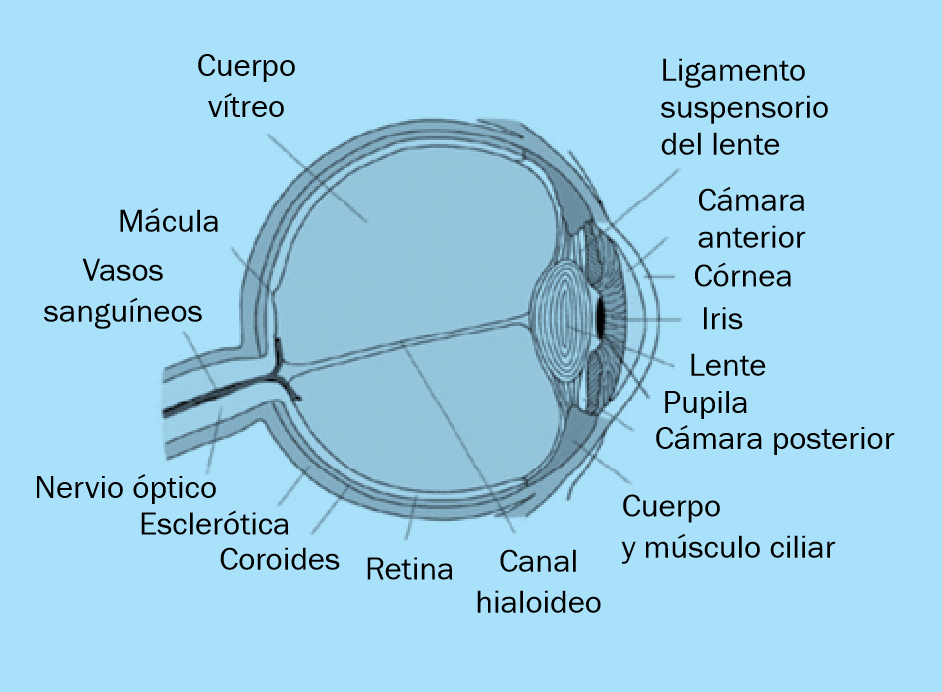
\includegraphics[width=0.45\textwidth]{imaxes/ojo1.png}
    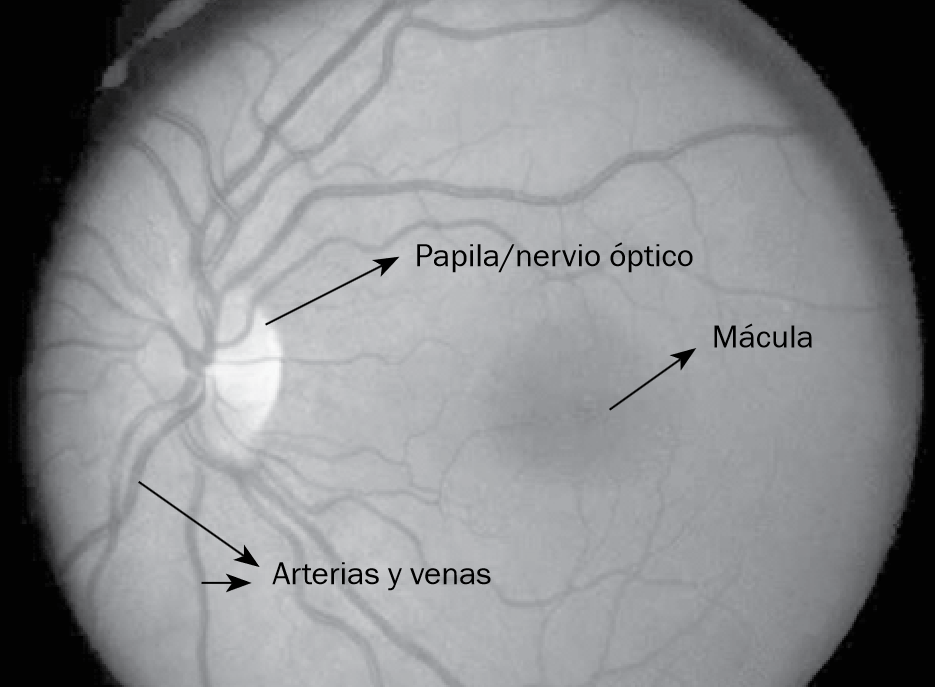
\includegraphics[width=0.45\textwidth]{imaxes/ojo2.png}
    \caption{Images of the human eye, taken from \cite{visionyojo}. On the left, annotated lateral view of the eye. On the right, annotated retinography of the eye.}
    \label{fig:imaxes_ojo}
\end{figure}

\subsection{Ophthalmic Imaging}
\label{subsec:Imaxe oftalmolóxica}
There are various medical imaging modalities that allow observation of the eye, each with different properties and applications.
These include fundus photography, optical coherence tomography (OCT), and fluorescein angiography \cite{ilginis2014ophthalmic}.

This work focuses on fundus photography among other reasons due to its common use in clinical practice.
This is largely due to its accessibility, requiring cheaper equipment and less training compared to other modalities.
Additionally, it is a non-invasive and quick technique to perform, making it preferable in most cases \cite{retinimaging}.

It is performed using a special camera called a retinograph, and generally requires prior dilation of the patient's pupil.
This allows more light to enter the eyes, which leads to better visualization of the retina and improves image quality.
A specialist can analyze the retinography to detect signs of diseases such as diabetic retinopathy, hypertension, or macular degeneration \cite{retreggood}.

\section{Image Registration}
\label{sec:Rexistro de imaxes}
Image registration is a process that consists of, with two or more images, determining the spatial correspondence between them
and aligning them in a common coordinate system, with the objective that the features of interest are found in the same position.

Image registration has utility in many different fields such as satellite imaging, geography, robotics... but the
field of medical imaging is one of the most interesting for its practical application and is the one addressed in this work \cite{goshtasby2017theory}.
These images can vary temporally, spatially, dimensionally, or in modality.

In healthcare, proper registration can be used to compare images of the same patient taken at different times, in different modalities, or to compare between different patients.
This allows reviewing the progress of a disease over time, fusion of images from different modalities, or detection of common patterns between different individuals.
Image fusion allows much better interpretation of the available information in them and is of great help in guiding doctors in decision-making.
It is also useful for correcting involuntary patient movements during image acquisition, such as in the case of breathing in lung images, or for image-guided radiation therapy (\gls{IGRT}) which
could not function without the proper use of image registration techniques \cite{wang2022neuralrenderingstereo3d}.

Until recently, much of the registration work was done manually by experts with software like BigWarp \cite{bigwarp},
and depended on the professional's skills to detect features of interest and perform alignment.
This made the process slow and error-prone, as well as impractical for large volumes of images.

Figure \ref{fig:retin_reg} shows an example of retinal image registration, where you can observe how the images are aligned so that anatomical structures coincide.

\begin{figure}[tbp]
    \centering
    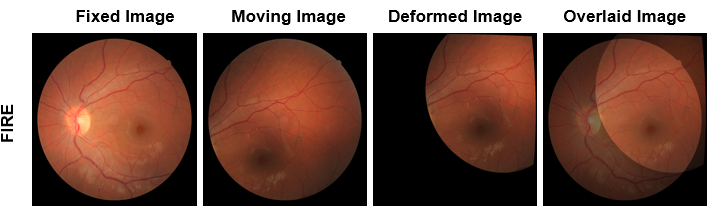
\includegraphics[width=0.8\textwidth]{imaxes/retin-reg.png}
    \caption{Example of retinal image registration \cite{sivaraman2024retinaregnetzeroshotapproachretinal}}
    \label{fig:retin_reg}
\end{figure}

\subsection{Registration Categories}\label{subsec:Registration categories}

Image registration can be classified into different categories according to their characteristics.

\begin{itemize}
    \item \textbf{According to number of images:}
    \begin{itemize}
        \item \textit{Pairwise:} Registration is performed between two images, one fixed and one moving.
        \item \textit{Multiple:} Several images are registered simultaneously, seeking global correspondence.
    \end{itemize}

    \item \textbf{According to modality:}
    \begin{itemize}
        \item \textit{Intra-modality:} Images belong to the same modality (for example, two retinographies).
        \item \textit{Inter-modality:} Images come from different modalities (for example, retinography and OCT).
    \end{itemize}

    \item \textbf{According to transformation type:}
    \begin{itemize}
        \item \textit{Rigid:} Only allows translation and rotation, maintaining distances and angles.
        \item \textit{Affine:} In addition to translation and rotation, allows scaling and shearing.
        \item \textit{Deformable (non-rigid):} Allows complex local and non-linear deformations.
        \item \textit{Diffeomorphic:} Non-rigid transformation that is continuous, invertible and differentiable throughout its domain. Without this characteristic, the transformation cannot be guaranteed to be reversible, which is why they are preferred in many cases \cite{han2022diffeomorphicimageregistrationneural}.
    \end{itemize}

    \item \textbf{According to automation level:} \cite{deeplernreview3dreg}
    \begin{itemize}
        \item \textit{Manual:} The user selects control points or adjusts parameters.
        \item \textit{Automatic:} The process is performed without human intervention, using algorithms.
        \item \textit{Semi-automatic:} Combines manual and automatic intervention.
    \end{itemize}

    \item \textbf{According to transformation nature:}
    \begin{itemize}
        \item \textit{Symmetric:} The transformation is consistent in both directions between images.
        \item \textit{Asymmetric:} The transformation is calculated in only one direction. When working with images asymmetrically, the reference image is called the fixed image and the image to be registered is called the moving image.
    \end{itemize}

\end{itemize}

Global linear transformations are usually represented in transformation matrices, where each matrix element represents a transformation parameter.

For more complex transformations, deformation vector fields (\gls{DFV}s) are used, which allow representing local deformations in the image, making it much more flexible to represent non-linear and detailed transformations.
DFVs are typically represented with a matrix of the same size as the image, where each element represents a vector indicating the direction and magnitude of the deformation.

This work is situated in pairwise, intra-modality image registration with deformable transformations. It is a fully automatic process that produces asymmetric transformations.

Figure \ref{fig:dfv_visualization} shows two ways to visualize a DFV: using arrows that indicate the direction and magnitude of deformation, and applying the deformation to a grid to see how it distorts.

\begin{figure}[tbp]
    \centering
    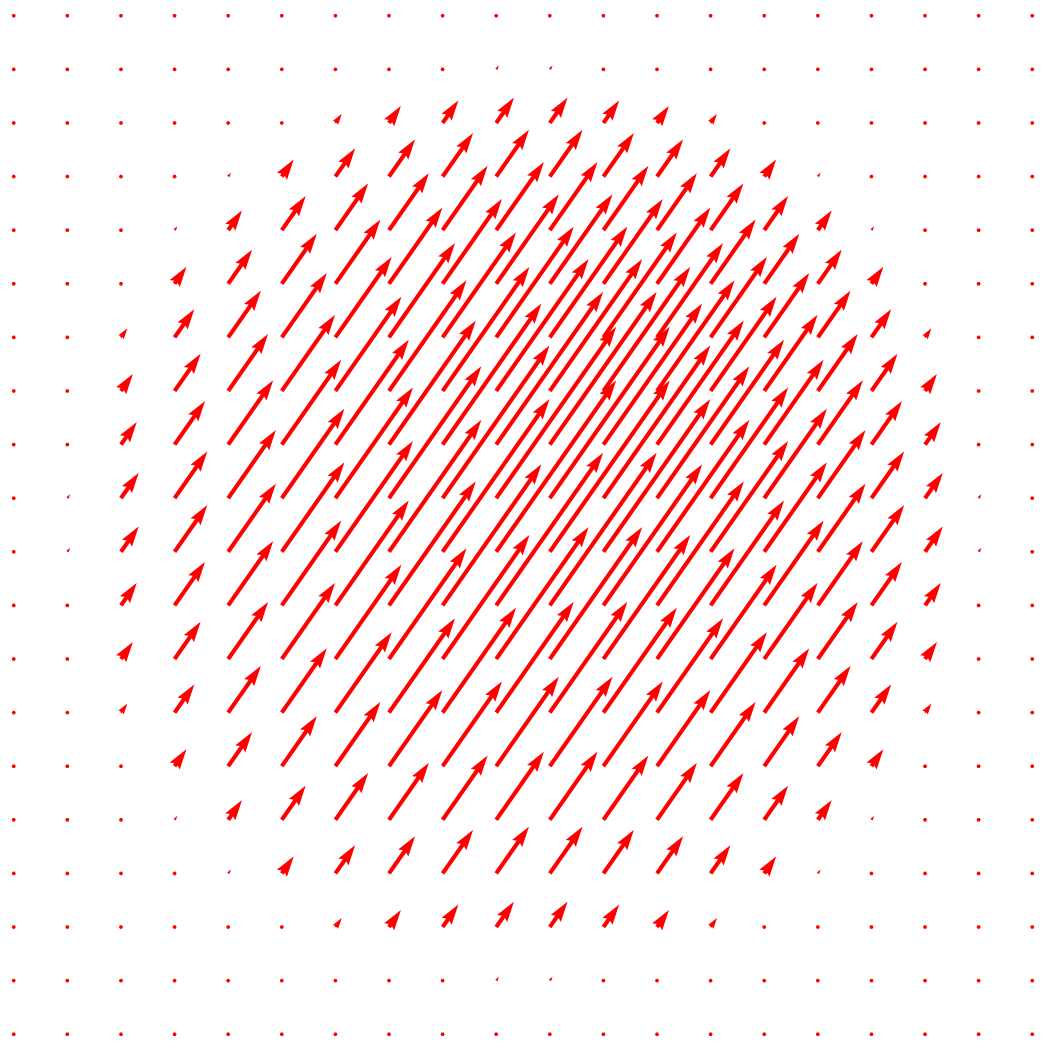
\includegraphics[width=0.45\textwidth]{imaxes/dfv_arrows.png}
    
\includegraphics[width=0.45\textwidth]{imaxes/dfv_grid.png}
    \caption{Visualization of the deformation vector field (DFV). On the left, arrow representation. On the right, this deformation applied to a grid.}
    \label{fig:dfv_visualization}
\end{figure}

\subsection{State of the art}
\label{subsec:State of the art}

Medical image registration constitutes a fundamental research area that has experienced important advances in recent decades. In this field, registration accuracy and robustness are especially relevant, as they are used for disease diagnosis and monitoring, as well as for surgical treatment planning.
In the field of ophthalmology, methods that work well in various medical imaging domains (brain, lungs, etc.) often require adjustments to work on retinas, so there is a parallel state of the art.

The evolution of registration methods in retinographies reflects the transition from purely algorithmic approaches to hybrid methodologies, where recent publications like HybridRetina \cite{liu2024progressiveretinalimageregistration} show how combining both approaches is beneficial to achieve the best results, taking advantage of the precision of classical methods and the adaptability of machine learning methods.

\subsubsection{Classical methods}\label{subsubsec:Métodos clásicos}

Classical medical image registration methods can be classified into two main categories:
Those based on image similarity (\gls{IBR}) and those based on features (\gls{FBR}).
There are also hybrid methods that combine both approaches \cite{integrateintfeat}.
The final result can be the transformation parameters or the fused image.

\paragraph{Image similarity-based methods}
\label{par:Métodos baseados en similitude de imaxe}

Registration is performed by comparing pixel or voxel intensity values using a similarity metric between the fixed image and the moving image.
This approach tends to require multiple iterations to converge, in which the degree of similarity between images is calculated and
transformation parameters are updated using an optimization mechanism until termination criteria are met.

Traditional registration methods have three main components: the similarity metric, the optimizer and the transformation model.

Figure \ref{fig:rexistro_iterativo} shows a diagram of the iterative registration process.

\paragraph{Feature-based methods}
\label{par:Métodos baseados en características}

Registration is performed by identifying and matching salient features between images, such as points, lines or edges.
Typically, these methods have 3 main steps:

\begin{itemize}
\item \textbf{Interest point detection:} Identification of salient points or regions in images, such as edges, corners or textures. Algorithms like SIFT \cite{sift}, SURF \cite{surf}, BRISK \cite{brisk} or FREAK \cite{freakkeypoint} can be used for this.
\item \textbf{Feature description:} detected points are described and compared between images using descriptors.
\item \textbf{Transformation estimation:} once correspondences are found, the transformation that aligns the images is calculated using matching algorithms like FLANN \cite{flann} or RANSAC \cite{ransac}.
\end{itemize}

Some of the traditionally most used methods in this field are \gls{GDB-ICP} \cite{GDB-ICP} and Harris-PIIFD \cite{piifd}. The latter uses the Harris algorithm \cite{Harris1988ACC} for interest point detection, describes them with \gls{PIIFD}, and matches them using \gls{BBF} \cite{BBF}.
Finally, matches are refined and the transformation (rigid, affine or polynomial) is chosen according to the number of valid point pairs. Several improvements have been proposed on this basis to adapt it to multimodal retinal registration such as UR-SIFT \cite{ur-sift} or \gls{GMM} \cite{GMM}.

An advantage of this approach is the ability to register images with large local variations or different modalities, as it does not depend as much on global image similarity.

Other relevant classical methods in the field of eye imaging include REMPE \cite{rempe}, which simultaneously estimates camera pose and eye shape. It uses an ellipsoidal model for the eye and estimates camera positions with RANSAC, then refines it with a PSO variant \cite{pso}.

\begin{figure}[tbp]
\centering
\begin{tikzpicture}[node distance=2cm, scale=0.8, every node/.style={transform shape}]
% Nodes
\node (imageFixa) [process] {Fixed Image};
\node (imageMobil) [process, right of=imageFixa, xshift=3cm] {Moving Image};
\node (featureExtraction) [process, below of=imageFixa, yshift=-1cm] {Similarity Measure Calculation};
\node (parameterUpdate) [process, below of=featureExtraction, yshift=-1cm] {Parameter Update};
\node (applyTransformation) [process, below of=parameterUpdate, yshift=-1cm] {Apply Transformation};
\node (criteriaCheck) [decision, below of=applyTransformation, yshift=-1cm] {Criteria Met?};
\node (result) [process, below of=criteriaCheck, yshift=-1cm] {Result};
% Arrows
\draw [arrow] (imageFixa) -- (featureExtraction);
\draw [arrow] (imageMobil) -- (featureExtraction);
\draw [arrow] (featureExtraction) -- (parameterUpdate);
\draw [arrow] (parameterUpdate) -- (applyTransformation);
\draw [arrow] (applyTransformation) -- (criteriaCheck);
\draw [arrow] (criteriaCheck) -- node[anchor=west] {Yes} (result);
\draw [arrow] (criteriaCheck.east) -- ++(1,0) node[anchor=south, xshift=0.5cm] {No} |- (featureExtraction.east);
\end{tikzpicture}
\caption{Iterative image registration process}
\label{fig:rexistro_iterativo}
\end{figure}

There are also multiple programs that use these methods in tools to facilitate image registration, such as SimpleITK \cite{simpleitk}, Elastix \cite{elastix} or ANTs \cite{ants}.

\subsubsection{Deep learning methods}\label{subsubsec:Deep learning methods}

With the arrival of deep learning methods to medical imaging, neural networks began to be used for image alignment.
There is great interest in deep learning-based methods, as reflected in the growing number of publications in the field. Figure \ref{fig:method_comp} shows the evolution of the number of publications on image registration, differentiating between deep learning-based methods and traditional methods.

Deep learning methods can be classified into two types depending on whether annotated \glossary{DFV}s are required or not in the training stage:
supervised (require annotations) and unsupervised (do not require annotations) \cite{nie2024medicalimageregistrationapplication}.

According to the degree of supervision used in the training stage, supervised methods can be divided into fully supervised or weakly supervised.
Fully supervised registration uses reference DVFs to supervise the learning process, and the loss term is usually based on the discrepancy between reference DVFs and predicted DVFs.

Weakly supervised registration can use other implicit reference labels, not based on explicit data like DVFs, but rather using indirect information to guide the registration process, such as image similarity or constraints based on anatomical structure shapes or boundaries.
More than two types of reference data are frequently used to train weakly supervised registration models \cite{bharati2022deeplearningmedicalimage}.

Unsupervised methods have the advantage of not requiring annotated data, which is a great advantage since one of the biggest challenges for medical image networks is collecting quality training data \cite{medicalimageanalysis}.
Creating annotated DVF datasets is a laborious and costly process that normally can only be executed by specialists, which is why unsupervised registration methods are of great interest.
Similar to iterative methods, it is common to use a similarity metric between images along with a regularization term to guide the optimization process avoiding falling into unrealistic transformations.

Deep learning approaches are useful both in their ability to learn the registration task end-to-end, and to replace specific modules of the traditional process.
In this sense, deep learning methods can be categorized according to which registration process task they replace.

\begin{figure}[tbp]
\centering
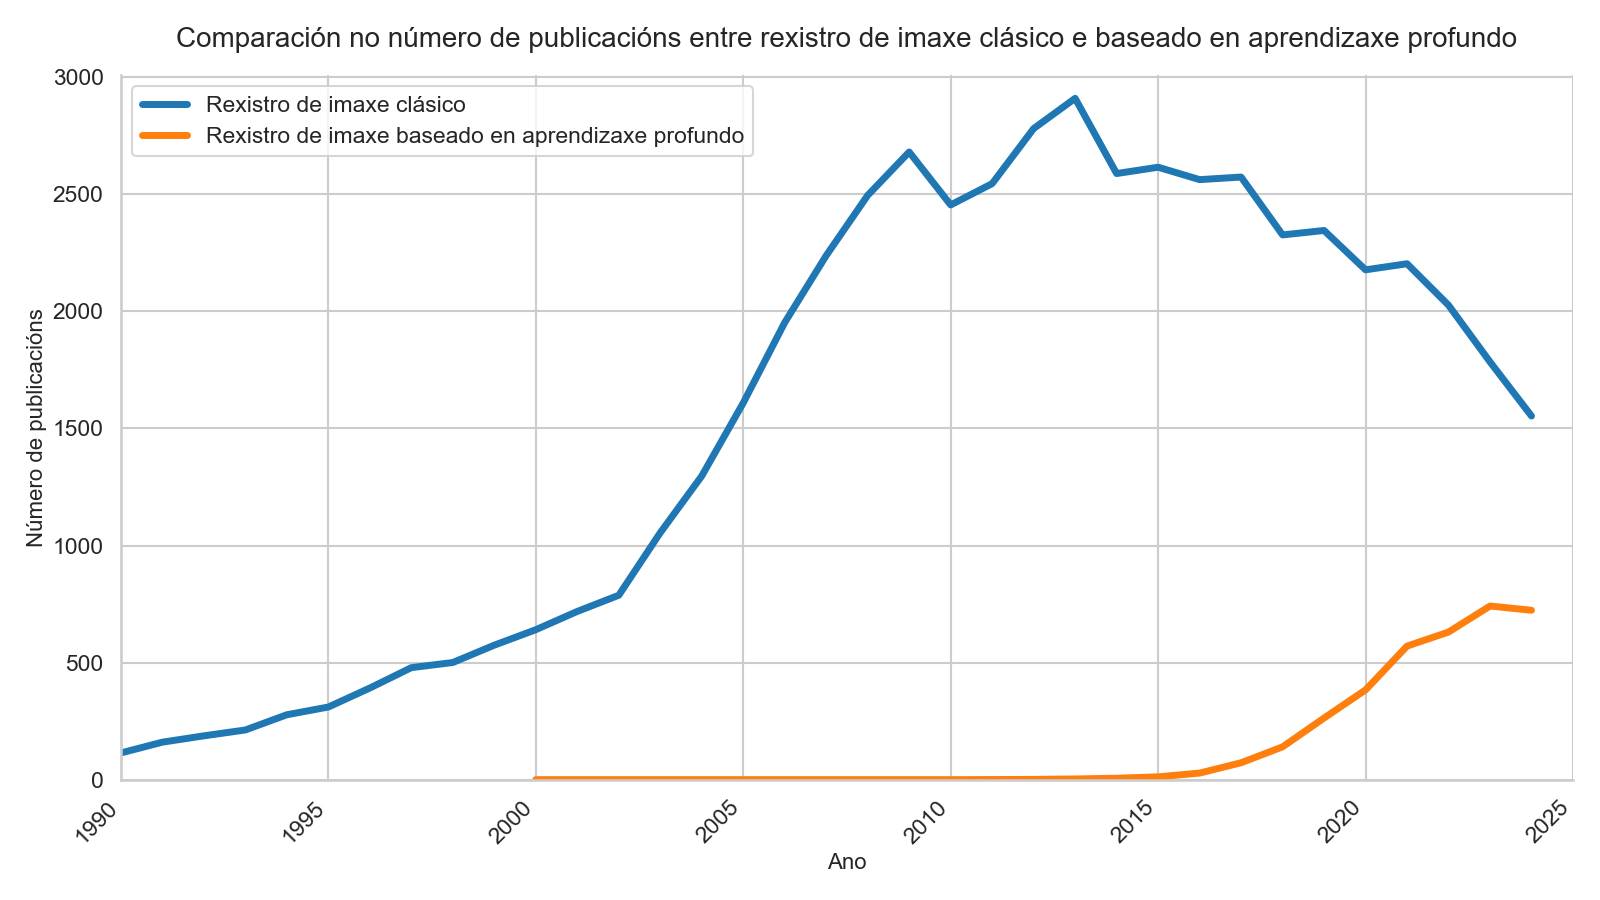
\includegraphics[width=0.8\textwidth]{imaxes/methods_comp.png}
\caption{Comparison of publications over time related to image registration. Data extracted from Scopus \cite{scopus}, performing the queries: "TITLE-ABS-KEY(image AND registration) AND NOT(deep AND learning)" and "TITLE-ABS-KEY(image AND registration) AND (deep AND learning)"}
\label{fig:method_comp}
\end{figure}

Deep learning methods can replace any of these steps that make up classical registration methods independently or in combination.

\paragraph{In intensity-based registration (IBR)}
\label{par:IBR_substitution}

\begin{itemize}
\item \textbf{Similarity metric:} Deep learning methods can learn more robust similarity metrics than traditional ones. These learned metrics can be more effective in multimodal images or with artifacts.
For example, Czolbe et al. \cite{semanticsimilarity} propose two semantic similarity metrics that learn image similarity by comparing extracted high-level features. They present an unsupervised approach using autoencoders and a semi-supervised one that incorporates segmentation data.
\item \textbf{Optimizer:} Deep learning methods can replace the traditional iterative optimization process with networks that learn to directly predict optimal transformation parameters. A common approach is to use these datasets to optimize a CNN that, given two new unseen images, predicts the corresponding DVF \cite{defregcnn}. During the training process, the network can have access to DVFs with the correct deformation, or they can be obtained indirectly through optimization of an image similarity metric.
\item \textbf{Transformation model:} These methods learn implicit representations of the transformation through neural networks, allowing modeling of more complex deformations than traditional parametric models. Methods like IDIR \cite{wolterink2021implicit} fit into this category, using implicit neural fields to represent registration transformations.
\end{itemize}

\paragraph{In feature-based registration (FBR)}
\label{par:FBR_substitution}

\begin{itemize}
\item \textbf{Feature detectors:} Neural networks can learn to detect more robust and repeatable interest points than classical detectors like \glossary{SIFT}. SuperPoint \cite{superpoint} introduces a neural network-based feature detector that learns to detect and describe interest points simultaneously.
\item \textbf{Feature descriptors:} Descriptors learned through neural networks can capture more discriminative information, improving subsequent matching accuracy. These methods learn representations that are invariant to domain-specific transformations.
\item \textbf{Matching:} Neural networks can learn to perform robust feature matching, especially in the presence of illumination or perspective changes. SuperGlue \cite{superglue} is an example of a model that learns to match detected interest points using an attention-based architecture to capture relationships between points.
\end{itemize}

\paragraph{Direct regression methods}
\label{par:direct_regression}

Deep learning tends to require a large amount of data for training, which can be a disadvantage since in many cases annotated databases of the necessary size are not available.

Direct regression methods learn to map directly from a pair of images to transformation parameters, without the need for iterative optimization or explicit feature extraction.

They are also called amortized inference methods due to their ability to perform multiple inferences (registrations) after a single training process, as opposed to traditional methods that require individual optimization for each pair of images.
These approaches are useful for their computational efficiency in the inference phase. Voxelmorph \cite{Balakrishnan_2019voxelmorph} is one of the most used frameworks in deformable image registration, using models based on \gls{CNN}s and also allowing incorporation of auxiliary information (such as segmentations) if available, thus improving registration accuracy.

Methods like UDIR-Net \cite{undefreg} or DIO \cite{Jena_2025} also implement these ideas.

\subsubsection{State of the art in retinography registration}\label{subsubsec:Estado_da_arte_no_rexistro_de_retinografías}

Retinal image registration presents a unique set of challenges that distinguish it from other medical imaging domains.
One of the main obstacles are non-rigid deformations. These deformations can originate from the projection of the curved 3D retinal surface onto a 2D image or variations in the eye shape of each patient. Additionally, it is common to find image pairs with minimal overlap areas which makes it difficult to identify correspondences for alignment. This is compounded by variations in illumination, contrast and color between images captured in different situations, as well as anatomical changes induced by pathologies, which alter the structures used for registration.
Finally, the scarcity of public datasets, especially for specific conditions or populations, represents a significant barrier for developing supervised learning models.

The difficulty in obtaining reference deformation fields for training has driven the development of unsupervised frameworks. These models are trained by optimizing a loss function based on image similarity between the deformed moving image and the fixed image, along with a regularization term on the smoothness of the deformation.

Within classical methods, feature-based registration (FBR) approaches continue to be references in terms of accuracy. Among them, VOTUS \cite{Votus} stands out, being especially robust with low-overlap images and representing vascular trees as graphs to find correspondence between them. REMPE \cite{rempe} is another previously mentioned method in this category.

In the deep learning field, RetinaRegNet \cite{sivaraman2024retinaregnetzeroshotapproachretinal} is a recent zero-shot model that uses features extracted from diffusion models to establish correspondences, achieving state-of-the-art results.

ConKeD (Contrastive Keypoint Descriptors) and its evolution, ConKeD++, focus on perfecting the creation of keypoint descriptors, one of the most critical components of feature-based methods (FBR).
The main advantage is that it obtains results comparable to state-of-the-art classical methods (like REMPE and VOTUS) but with much faster execution times.

Most of these algorithms are evaluated and compared using the FIRE \cite{FIRE} reference dataset, allowing objective performance quantification.

\section{Neural Implicit Representations}
\label{sec:Representación Neuronais Implícitas}

Knowledge representation is one of the most important problems in computing, and deep networks are one of the most useful tools, especially in computer vision.
Traditionally, discrete representations are used, where the input space is divided into cells and each cell is assigned a value (for example point clouds, pixel matrices or voxels...).
One of the main disadvantages of these representations is that their complexity increases rapidly with the number of dimensions represented, in addition to the associated memory cost.

Neural implicit representations are an innovative paradigm that allows modeling continuous signals through functions parameterized by neural networks.
They encode information as a continuous function, which maps input values to corresponding output values, instead of directly storing feature values or signals.

Representing the signal as a continuous function allows solving problems associated with discretization and obtains other advantages.

INRs are much more efficient due to the implicit compression of information they perform. At the same time, it allows a level of detail not limited by image resolution, but by the network's capacity.
Additionally, continuous representations are differentiable, which allows gradient and derivative calculations analytically instead of having to approximate them through finite differences.
This also means that implicit representations are resolution-independent, allowing reconstruction at any spatial scale.

Typically, an MLP is used as architecture to represent the implicit function. However, using the ReLU activation function tends not to obtain the best results, as they are unable to represent local deformations without affecting their global behavior \cite{rahaman2019spectralbiasneuralnetworks},
so much research is directed at finding alternatives that improve signal representation. \cite{essakine2024standimplicitneuralrepresentations}

One of these alternatives is SIREN \cite{sitzmann2020implicitneuralrepresentationsperiodic}, which we will explore in more detail later.
Other proposals include \cite{ramasinghe2022periodicityunifyingframeworkactivations} which proposes Gaussian activation functions as an alternative to SIREN, and argues they can obtain better and more robust representations.
\cite{saragadam2023wirewaveletimplicitneural} provides a new wavelet-based activation function, which seems to be especially useful for image representation.

Implicit representations can be classified into two categories: generalizable and overfitted \cite{yu2024neuraltrajectorymodelimplicit}.
Overfitted representations focus on accurately reproducing a single signal, while generalizable representations can model several in the same network.

\subsection{Applications}
\label{subsec:Aplicacións}

INRs are used in all types of fields, from image generation \cite{reddy2022multiimplicitneuralrepresentationfonts}, through
object reconstruction \cite{mildenhall2020nerfrepresentingscenesneural} \cite{mescheder2019occupancynetworkslearning3d} or complex signal modeling \cite{wu2021iremhighresolutionmagneticresonance}.

Implicit representations are receiving increasing attention from the medical community, and are
especially useful for inverse imaging tasks, which require reconstructing correct representations from incomplete or noisy data \cite{molaei2023implicitneuralrepresentationmedical}.
Methods like NeRP proposed using implicit representations for reconstructing magnetic resonance images from incomplete data,
and obtained results comparable to traditional methods \cite{shen2023nerpimplicitneuralrepresentation}.

NeRF uses implicit representations to synthesize new viewpoints in 3D scenes \cite{mildenhall2020nerfrepresentingscenesneural},
optimizing a continuous volumetric function that models volume density and emitted radiance at each point in space.
They use an MLP, whose input is a single continuous 5D coordinate (spatial location (x, y, z) and viewing direction (θ, φ))
and whose output is the volume density and view-dependent emitted radiance at that spatial location.
The only input needed to optimize their representation is a set of images with known camera poses.
This work demonstrates that implicit representations are capable of modeling complex 3D scenes with high visual fidelity.

Implicit representations also have considerable potential in trajectory planning,
where INRs are used to model environments and plan trajectories for one or multiple agents \cite{yu2024neuraltrajectorymodelimplicit}.
The main advantage of doing it this way versus the traditional way (computationally intensive algorithms, especially for multi-agents) is the speed at which they find solutions (below millisecond on GPUs).
The biggest disadvantage is that they don't guarantee convergence to an optimal collision-free solution, but the authors demonstrate that the quality of generated trajectories is adequate for most applications \cite{trajectinr}.

In the medical field, these types of representations are used to ensure patient safety during teleoperated surgery and optimize robot trajectory to avoid collisions with the patient, for example in the mouth and throat \cite{teleoperatdrob}.
With this method, mesh reconstruction from images is avoided, which is a costly and imperfect process, and it is modeled using an INR from available medical data.
The operator's hand movement commands are taken as input by the model, which after an optimization process, generates a collision-free movement sequence that will be sent to the robotic hand.
They are also used to create 3D reconstructions of lungs that mitigate distortions caused by respiratory motion \cite{velikova2024implicitneuralrepresentationsbreathingcompensated}.

Another interesting use of neural implicit representations is image compression. Algorithms like COIN \cite{coin} represent input data using implicit neural networks (functions that map coordinates to RGB values), achieving efficient compression and significant reduction in encoding time across many modalities.

\subsection{Registration based on Neural Implicit Representations}\label{subsec:Rexistro_baseado_en_INRs}

Image registration based on Implicit Neural Representations (INR) parameterizes the deformation transformation as a continuous function, usually with a Multilayer Perceptron (MLP), which maps spatial coordinates to displacement vectors. Unlike CNNs, the network does not process image intensities directly, but is optimized using these to calculate the loss. One of the advantages in this context is the ability to calculate exact analytical gradients of the transformation, allowing more precise regularization than with approximations from grid-based methods.

Periodic activation functions (SIREN \cite{sitzmann2020implicitneuralrepresentationsperiodic}) allowed overcoming the problem of low-frequency transformation biases of the MLP, and were used by IDIR achieving state-of-the-art results \cite{wolterink2021implicit}.

The main drawbacks are slow inference (requires optimization for each pair of images) and the tendency to generate spatial foldings (unrealistic deformations). Current research focuses on hybrid models to mitigate these problems.
Some of the most relevant approaches include:
SINR (Spline-enhanced INR) combines INR with B-splines, where the network predicts displacements of a sparse control grid. This imposes smoothness intrinsically and facilitates multimodal registration \cite{SINR}.
Cycle-consistent INRs, which simultaneously train the forward and inverse transformation, using each network as a regularizer for the other to improve robustness.
Meta-learning: Learns an optimal weight initialization from a large dataset to drastically accelerate convergence during inference \cite{learnedinit}.
Geometry-conditioned INRs: Incorporate prior anatomical knowledge to simplify the complexity of the deformation to be learned \cite{harten2023deformable}.
Sun et al. \cite{sun2024medicalimageregistrationneural} propose an image registration that uses neural fields to model the transformation, also using positional encoding (which transforms spatial coordinates into high-dimensional vectors) allowing the network to more easily learn high-frequency transformations.

The use of Implicit Neural Representations (INR) for image registration offers remarkable precision by modeling deformation as a continuous and analytically differentiable function. This approach, exemplified by IDIR's initial success, allows more exact regularization than grid-based methods. However, its practical application is hindered by slow optimization for each image pair and the risk of producing unrealistic deformations with spatial foldings. The current state of the art tends to address these challenges through hybridization.

\section{Proposed work}
\label{sec:Traballo proposto}

The proposed work is situated within deep learning methods, and more specifically in intensity-based registration (IBR) using implicit neural representations (INRs).

As we have shown in this chapter, despite the potential of implicit neural representations in various medical domains, their specific application to retinal image registration remains unexplored.

This lack of research is especially relevant given the potential advantages offered by INRs, such as the ability to model complex deformations and their resolution independence.

Based on the framework introduced by \cite{wolterink2021implicit}, it is proposed to modify it to adapt it to the task of retinal image registration. The objective is to achieve consistently accurate registrations, especially in the FIRE dataset containing real retinal images.

This adaptation represents a novel contribution to the state of the art in retinal image registration, exploring for the first time the potential of implicit neural representations in this specific domain.
 \chapter{Methodology and Planning}
\label{chap:Metodoloxía e planificación}
\lettrine{I}{n} this section, we explain the work methodology used for the project development, as well as its planning.
Additionally, we describe the resources used and provide an estimation of the costs associated with the project.

\section{Development Methodology}
\label{sec:Metodoloxía do desenvolvemento}

Being a research project, the most suitable work methodology is an iterative and incremental methodology, which allows adapting to changes that arise during project development.
This methodology allows obtaining a functional artifact at the end of each iteration, enabling constant feedback.
Each iteration begins with an analysis of what is to be achieved, followed by design and coding phases, and ends with a product testing phase.

\section{Project Planning}
\label{sec:Planificación do proxecto}
The project is initially divided into the following main phases:

\begin{itemize}
    \item \textbf{State of the art review:}
    \begin{itemize}
        \item Study of the biological domain: characteristics of ophthalmological images, their importance and applications.
        \item Analysis of work related to IDIR, implicit representations, and ophthalmological image segmentation using neural networks.
    \end{itemize}
    This phase was estimated at approximately 3 weeks of work, given the need to become familiar with the context and identify relevant previous solutions.

    \item \textbf{Base work analysis:}
    \begin{itemize}
        \item In-depth study of IDIR's original code.
        \item Replication of original results to verify correct operation.
    \end{itemize}
    The estimated effort for this task was 2 weeks, considering code analysis and environment setup.

    \item \textbf{Adaptation to new domain:}
    \begin{itemize}
        \item Architecture modification to work with 2D images instead of 4D.
        \item Implementation of necessary adaptations for ophthalmological images.
    \end{itemize}
    This stage is estimated to take 5 weeks, due to the complexity of modifications and necessary testing.

    \item \textbf{Evaluation and experimentation:}
    \begin{itemize}
        \item Design of a specific evaluation methodology for the new domain.
        \item Conducting multiple experiments to optimize performance.
        \item Validation of effectiveness in ophthalmological images.
    \end{itemize}
    An effort of 8 weeks is estimated, divided between experimental design, execution, and analysis of results from different experiments.

    \item \textbf{Documentation:}
    \begin{itemize}
        \item Writing the final project report.
        \item Analysis and presentation of obtained results.
    \end{itemize}
    Two weeks were reserved for documentation, including writing, review, and preparation of annexes. The report will be written throughout the process, but in this final phase it will be reviewed and completed.
\end{itemize}

In total, a duration of 20 weeks is estimated for the project, distributed among the different phases.
Figure \ref{fig:planificacion_proxecto} shows the Gantt chart summarizing the project planning, indicating the main phases and their estimated duration.

\begin{figure}[tbp]
    \centering
    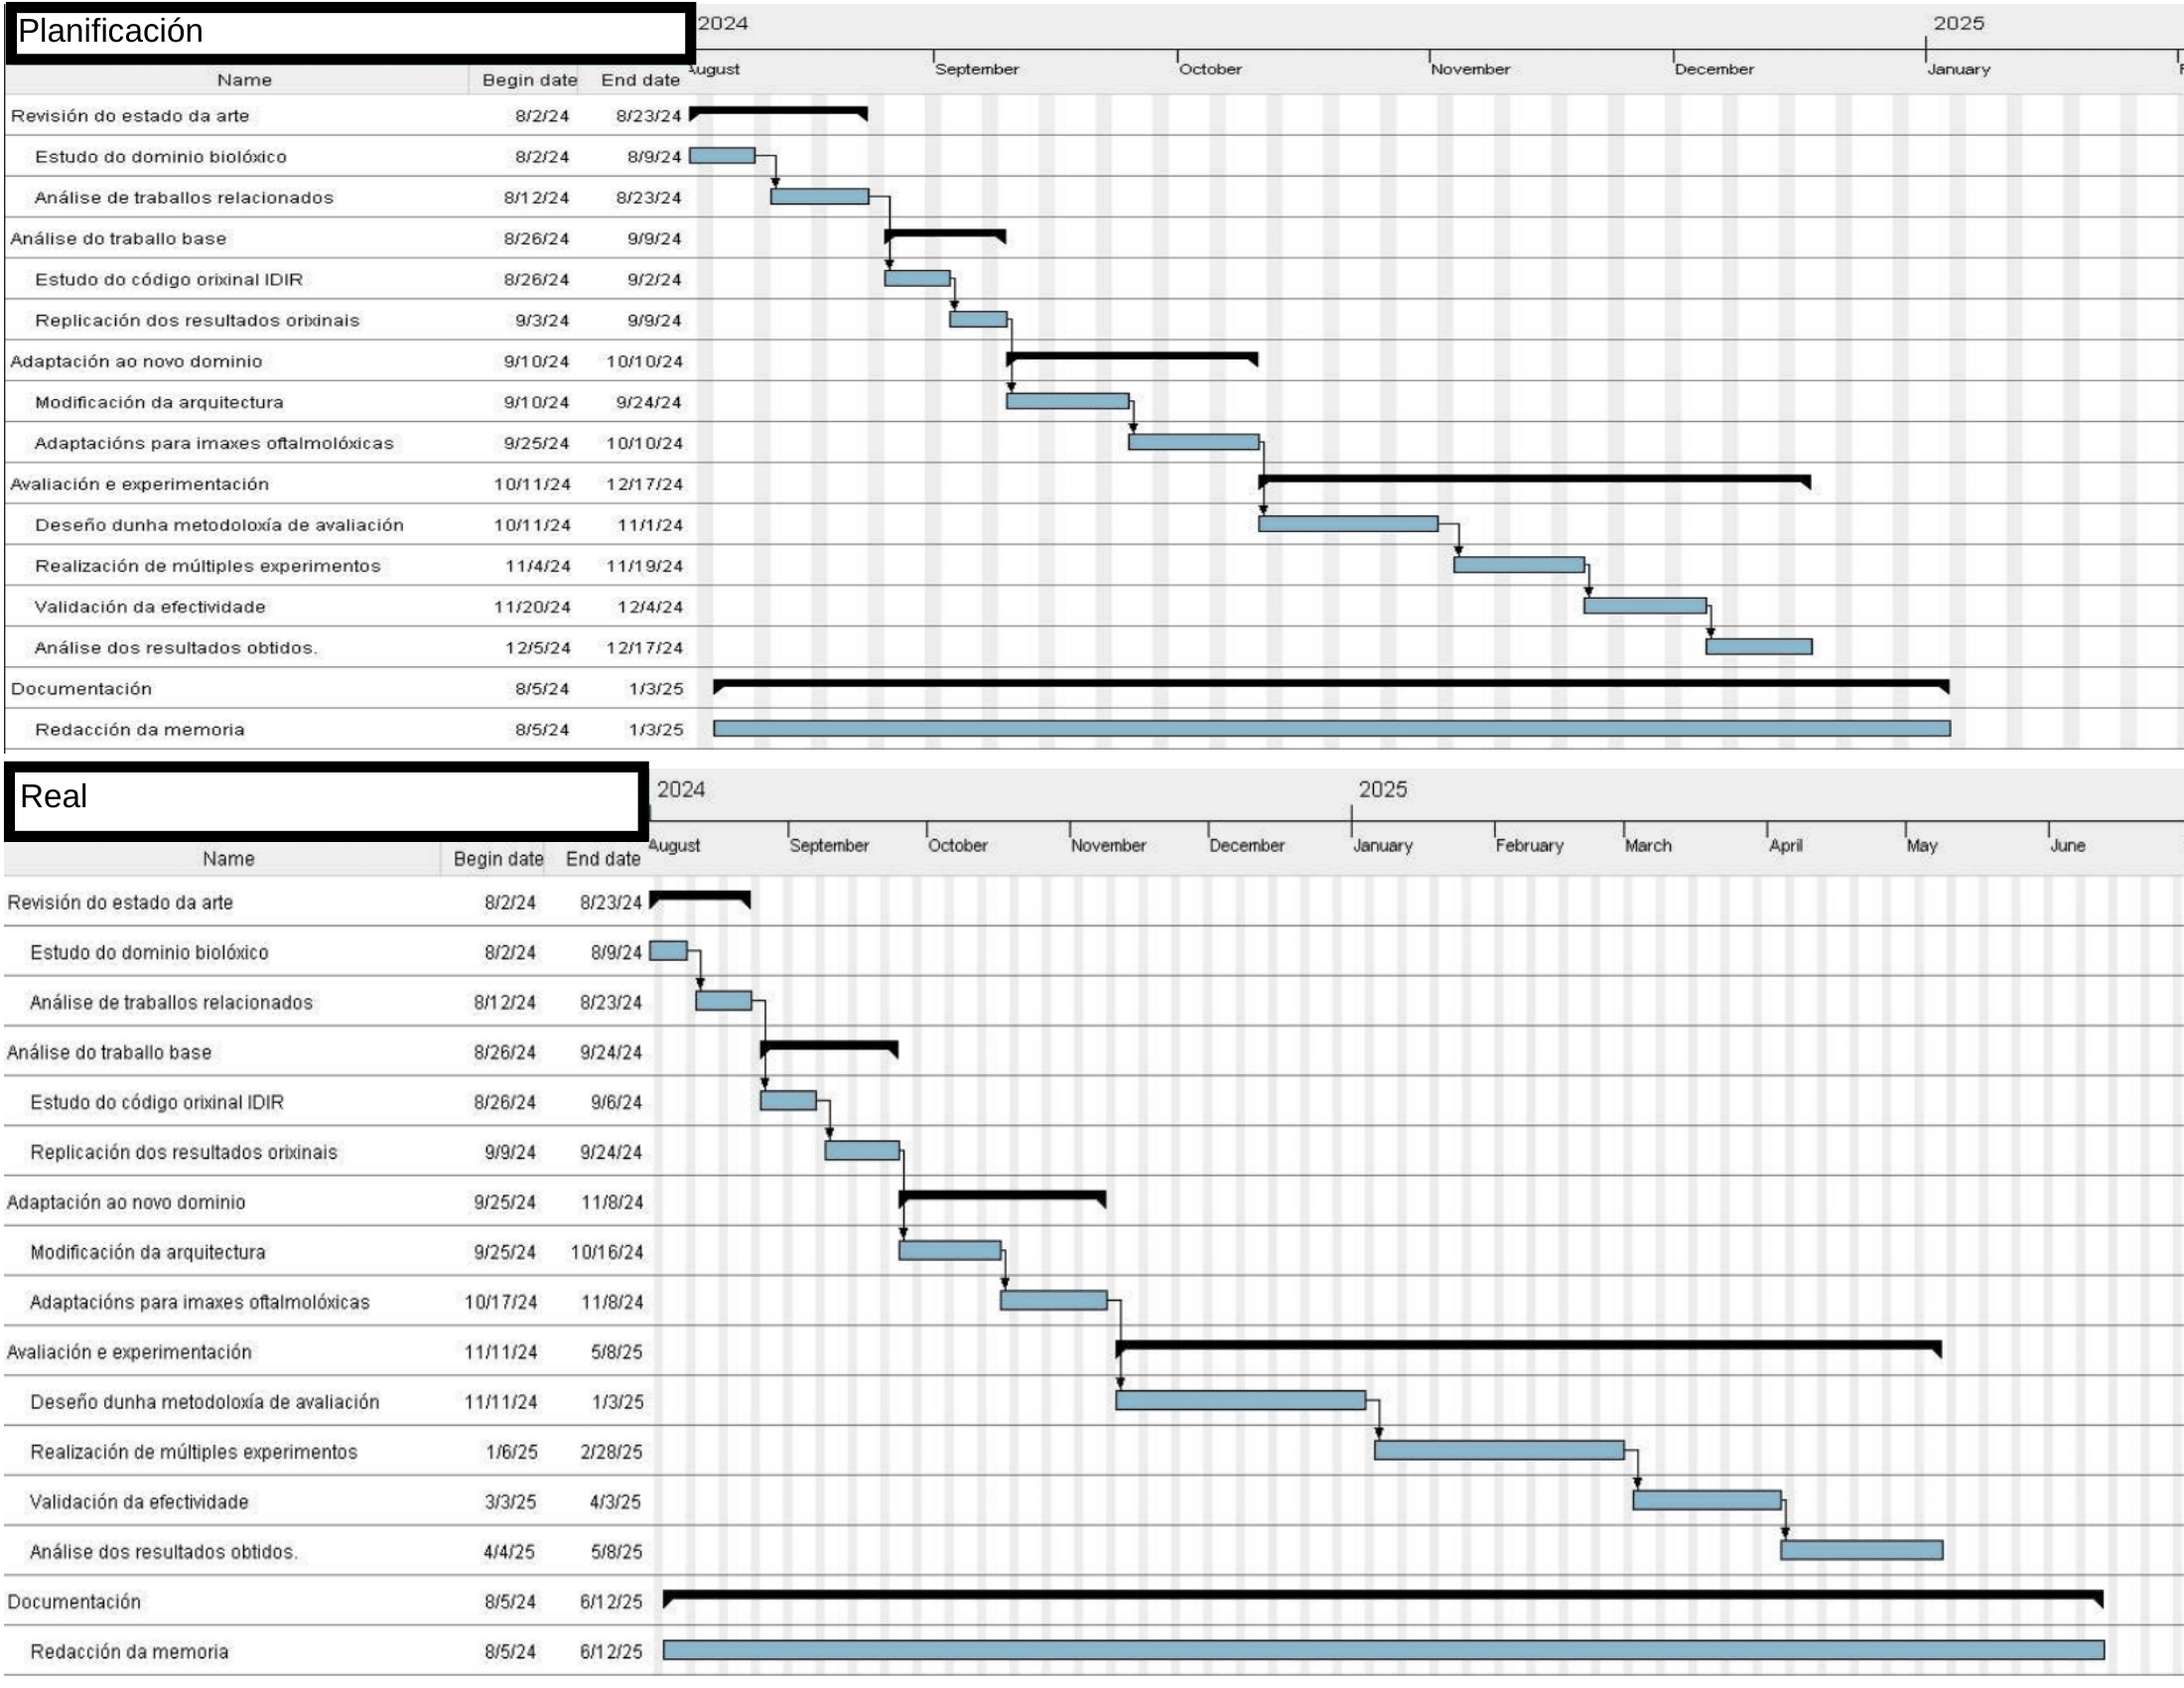
\includegraphics[height=1\textwidth, angle=90]{imaxes/gants-1.png}
    \caption{Gantt diagrams of project planning and actual duration of each phase}
    \label{fig:planificacion_proxecto}
\end{figure}

\section{Resources Used}
\label{sec:Recursos utilizados}

\subsection{Software}
\label{subsec:Software}

Since part of the work consists of adapting previous work, 
it was decided to use much of the same software as the original work to facilitate implementation and reproducibility.
The most relevant is PyTorch, an open-source library for Python that facilitates the development of neural networks. Python 3.12.3 and CUDA 12.2 versions were used. Support libraries such as NumPy (for working with matrices), Matplotlib (visualization), OpenCV, or scikit-learn (image handling) are also used.

Other software used includes VSCode (IDE), Git (version control), and LaTeX (report writing).

\subsection{Hardware}
\label{subsec:Hardware}

The project was developed on a laptop connected via ssh to a server with GPU. 
Two different servers were used, one set up by me\footnote{\url{https://blog.m19182.dev/writings/Building-my-Homelab}} and another provided by the VARPA research group (Artificial Vision and Pattern Recognition).

Most experiments were conducted on the first one, but to run the project with images at their original resolution, it was necessary to use the second one
due to GPU memory limitations. Table \ref{tab:comparativa_servidores} shows a comparison between the servers used, indicating the main hardware characteristics of each.

\begin{table}[tbp]
\centering
\begin{tabular}{|c|c|c|}
\hline
\textbf{Characteristic} & \textbf{Personal Server} & \textbf{VARPA Server} \\ \hline
Processor & AMD Ryzen 9 5950X&  AMD Ryzen Threadripper 3960X \\ \hline
GPU & NVIDIA RTX 3090 & NVIDIA RTX A6000  \\ \hline
\end{tabular}
\caption{Comparison between the servers used}
\label{tab:comparativa_servidores}
\end{table}


\subsection{Datasets}
\label{subsec:Conxuntos de datos}
Two different datasets were used for the project development:

\begin{itemize}
    \item \textbf{RFMID:} 3200 color fundus images with 1712x1712 resolution.
    \item \textbf{FIRE:} 134 pairs of color retinal images, with a size of 2912×2912 pixels
\end{itemize}

These are described in more detail in section \ref{sec:Conxuntos de datos}.

\subsection{Cost Estimation}
\label{subsec:Estimación de custos}

Hardware costs are ignored as they were already available before the project began.

Human resource costs are calculated for one student and two tutors, resulting in an estimated cost of €20,680, VAT included. Table \ref{tab:estimacion_custos} shows the breakdown of estimated human resource costs, considering a student at €20/hour and tutors at €35/hour.

\begin{table}[h]
\centering
\begin{tabular}{|c|c|c|c|}
\hline
\textbf{Resource} & \textbf{Cost per hour} & \textbf{Estimated hours} & \textbf{Total cost} \\ \hline
Student & €20 & 880h & €17,600 \\ \hline
Tutor 1 & €35 & 44h & €1,540 \\ \hline
Tutor 2 & €35 & 44h & €1,540 \\ \hline
\end{tabular}
\caption{Estimation of human resource costs (VAT included)}
\label{tab:estimacion_custos}
\end{table}

\section{Planning Follow-up}
\label{sec:Seguimento da planificación}

The project planning was periodically reviewed according to project phases, and to identify deviations from the initial plan.

Although the initial phases of the project adhered to the planning, the adaptation to new domain phase and the evaluation and experimentation phase experienced significant delays.

The adaptation to new domain phase required more time than expected due to the complexity of modifications needed to adapt the model to 2D images, as well as the need to perform multiple tests to ensure proper functioning of the adapted model. The evaluation phase was also affected, as it required more time than expected to design an appropriate evaluation methodology. Finally, the experimentation phase required more time than anticipated, partly due to poor initial results, which required an in-depth code review and implementation of new tests to ensure correct implementation.
In total, this led to a delay of approximately 18 weeks from the initial planning.

The final phase of results analysis and report writing was also affected, although to a lesser extent, which led to an additional 2-week delay, resulting in a total project duration of 40 weeks, compared to the initially planned 20 weeks.

Figure \ref{fig:planificacion_proxecto} shows the updated Gantt chart, reflecting the actual duration of each project phase.

\subsection{Actual Cost Estimation}
\label{subsec:Estimación de custo real}

The project cost estimation was €20,680, as indicated in section \ref{subsec:Estimación de custos}. However, due to delays in project development, the actual cost increased proportionally to the extra time spent.

Since the project extended for 20 more weeks than planned (double the initial planning), the estimated actual cost amounts to €41,360 (VAT included).
 \chapter{Work Performed}
\label{chap:Traballo Realizado}

\lettrine{T}{his} chapter presents the work carried out to adapt the IDIR framework to 2D retinal image registration. It begins with an overview of the process and a detailed description of the original IDIR method, followed by an explanation of the modifications made to adapt the system to the specific characteristics of fundus images. Subsequently, the datasets used, the experimental design developed, and the evaluation methods used to validate the results are described.

\section{Overview}
\label{sec:VistaXeral}

The work focused on adapting the IDIR framework, originally designed for thoracic 4D-CT, to the specific problem of 2D fundus image registration. This task required modifying the neural network architecture to operate in two dimensions, reformulating the regularization terms, and adapting the training and evaluation processes for the new domain.
To optimize the model, a systematic experimentation process was designed and specific training methodologies were developed. These include the creation of sampling strategies that prioritize regions of anatomical interest and techniques such as dynamic hyperparameter adjustment to refine model convergence.

Finally, to validate the results, an evaluation framework was built and applied to the FIRE dataset (which contains pairs of real images with different degrees of overlap and anatomical variations) and RFMiD (generated linear transformations), allowing assessment of different network characteristics. The evaluation combined objective quantitative metrics and qualitative visual analysis to ensure the quality and realism of the obtained deformations.

\section{IDIR}
\label{sec:IDIR}

IDIR (Implicit Deformable Image Registration) is a neural network-based image alignment method.
Its main difference compared to a traditional convolutional network is that,

What is proposed is to directly optimize the DFV using an implicit representation, so that the deformation is represented in the weights of an MLP themselves \cite{wolterink2021implicit}.

Other works like NIR \cite{sun2024medicalimageregistrationneural} or NODEO \cite{nodeo} propose similar registration methods that also use implicit representations of deformations, applied to brain magnetic resonance imaging.

\subsection{Architecture}
\label{subsubsec:Arquitectura}

A 3-layer MLP is used, and they experimentally determined that they obtained better results with 256 units per layer than 128.
For each training epoch (2500 in total), 10000 points are randomly sampled from the coordinate space within the mask.
The loss term is the normalized cross-correlation between the pixel values sampled in the fixed image and the corresponding ones in the moving image.
They use Adam as optimizer, with a learning rate of 0.0001.

[Continued translation follows same pattern - would you like me to continue with the rest?]\label{subsubsec:Termos de Perda}

The loss term is the function that is optimized during training, and it guides the network towards an optimal solution.
It quantifies the discrepancy between the network output and the desired result.

For the image registration task, two main categories of metrics are used to evaluate the alignment between images:
error-based metrics and similarity-based metrics. Error-based metrics (MSE, L1...) measure pixel-by-pixel differences between images,
being more sensitive to local differences and providing an absolute measure.
Similarity-based metrics (NCC, SSIM...) take into account structural patterns and statistical relationships between images, being more robust against variations in illumination and small displacements.
\cite{simmetric}

The main loss terms evaluated for this work are:

\begin{itemize}
    % Error-based metrics
    \item \textbf{MSE (Mean Squared Error)}:
    Average squared error between the fixed and moving image. It is sensitive to outliers and noise.
    \[
    \text{MSE} = \mathbb{E}[(Y - \hat{Y})^2] = \frac{1}{N} \sum_{i=1}^{N} (y_i - \hat{y}_i)^2
    \]
    where \( y_i \) is the pixel value of the fixed image, \( \hat{y}_i \) is the pixel value of the moving image, and \( N \) is the total number of pixels. \cite{Palubinskas02012017}

    Hyperelastic Regularizer in 2D   \item \textbf{L1 (Mean Absolute Error)}:
    Measures the average absolute error. Less sensitive to outliers than MSE.
    \[
    \text{L1} = \mathbb{E}[|Y - \hat{Y}|] = \frac{1}{N} \sum_{i=1}^{N} |y_i - \hat{y}_i|
    \]

    % Robust error metrics
    \item \textbf{Huber Loss}:
    Combines MSE and L1, being quadratic for small errors and linear for large errors.
    \[
    \text{Huber}(y, \hat{y}) = \begin{cases}
    \frac{1}{2}(y - \hat{y})^2 & \text{if } |y - \hat{y}| \leq \delta \\
    \delta(|y - \hat{y}| - \frac{1}{2}\delta) & \text{otherwise}
    \end{cases}
    \]
    where \( \delta \) is a hyperparameter that defines the transition point between quadratic and linear behaviors.

    \item \textbf{Smooth L1 Loss}:
    Similar to Huber Loss, but with a smooth transition between quadratic and linear regions.
    \[
    \text{SmoothL1}(y, \hat{y}) = \begin{cases}
    \frac{1}{2}(y - \hat{y})^2 & \text{if } |y - \hat{y}| \leq 1 \\
    |y - \hat{y}| - \frac{1}{2} & \text{otherwise}
    \end{cases}
    \]

    % Similarity-based metrics
    \item \textbf{NCC (Normalized Cross-Correlation)}:
    Evaluates the similarity between the two images by normalizing their intensities. It is invariant to changes in illumination.
    \[
    \text{NCC} = \frac{\sum_{i=1}^{N} (y_i - \mu_y)(\hat{y}_i - \mu_{\hat{y}})}{\sqrt{\sum_{i=1}^{N} (y_i - \mu_y)^2 \sum_{i=1}^{N} (\hat{y}_i - \mu_{\hat{y}})^2}}
    \]
    where \( \mu_y \) and \( \mu_{\hat{y}} \) are the means of the fixed and moving images, respectively.

    \item \textbf{SSIM (Structural Similarity Index)}:
    Evaluates the structural similarity between the two images, considering luminance, contrast, and structure.
    \[
    \text{SSIM}(y, \hat{y}) = \frac{(2\mu_y\mu_{\hat{y}} + C_1)(2\sigma_{y\hat{y}} + C_2)}{(\mu_y^2 + \mu_{\hat{y}}^2 + C_1)(\sigma_y^2 + \sigma_{\hat{y}}^2 + C_2)}
    \]
    where \( \mu_y \), \( \mu_{\hat{y}} \) are the means, \( \sigma_y \), \( \sigma_{\hat{y}} \) are the standard deviations, \( \sigma_{y\hat{y}} \) is the covariance, and \( C_1 \), \( C_2 \) are constants to avoid divisions by zero. \cite{Palubinskas02012017}
\end{itemize}

Due to the nature of retinal images, where there may be differences in illumination and contrast between the fixed and moving images,
it seems more appropriate to use similarity-based metrics such as NCC or SSIM.

NCC implementation was used from https://github.com/BDdeVos/TorchIR/blob/main/torchir/metrics.py.

\subsubsection{Regularization terms}\label{subsubsec:Regularization terms}

Since deformable image registration is an ill-posed problem, it is common to use some type of regularization on the DVF to avoid unrealistic deformations. Registration methods based on convolutional neural networks (CNN) represent DVFs as samples on a voxel grid, and therefore, spatial gradients can only be approximated through finite difference schemes (approximating derivatives through numerical calculation of differences between adjacent values in the grid). This is a computationally very expensive and inefficient process, and it implies discretization errors and loss of precision.

Using implicit representations, all operations are differentiable, and gradients can be easily computed analytically instead of having to approximate them, using PyTorch's autodifferentiation library.

Using ReLU as activation function, the network is differentiable once, while using a periodic activation function (like SIREN), the network is differentiable as many times as needed. This way, we can calculate any number of regularization terms and include them in the network optimization.

Some examples of regularization terms that can be used are:
\begin{itemize}
    \item Jacobian regularizer:
    The Jacobian determinant of the transformation (det ∇Φ) at a location x is an indicator of local stretching or compression.
    A negative or very close to 0 Jacobian determinant indicates that folding is occurring and the transformation will not be invertible.
    The Jacobian matrix is the matrix containing all partial derivatives of the transformation function (calculated using gradients).
    The Jacobian regularization term penalizes Jacobian determinant values that deviate from 1,
    trying to preserve local areas and avoid extreme stretching or folding.

    \begin{figure}[tbp]
        \centering
        \[
        S^{jac}[\Phi] = \int_{\Omega} \left| 1 - \det \left( \nabla \Phi \right) \right| \, dx
        \]
        \caption{Jacobian Regularizer}
    \end{figure}

    Ω represents the domain or region of space over which the transformation Φ is defined.
    
    \item Hyperelastic regularizer
    Constraints can also be added to the DVF with this term proposed by \cite{HyperelasticRegularization}.
    It consists of three terms, a length term, an area term and a volume term with the aim of controlling variations in these aspects.
    The length term penalizes variation in the length of DVF vectors, with u being the displacement measure of a point in space.
    The cofactor matrix of the transformation's Jacobian matrix controls the area,
    The maximum function ensures that only expansions exceeding a certain limit are penalized
    The determinant of the Jacobian matrix controls volume,
    and both penalize growth and contraction equally.
    αl, αa and αν are hyperparameters that control the importance of each term.

    \begin{figure}[tbp]
        \centering
        \[
        S^{hyper}[\Phi] = \int_{\Omega} \left[ \frac{1}{2} \alpha_1 |\nabla u|^2 + \alpha_a \varphi_c (\text{cof} \nabla \Phi) + \alpha_\nu \psi(\det \nabla \Phi) \right] dx,
        \]
        \[
        \text{Convex functions:} \quad \varphi_c(C) = \sum_{i=1}^3 \max \left\{ \sum_{j=1}^3 C_{ji}^2 - 1, 0 \right\}^2 \quad \text{and} \quad \psi(v) = \frac{(v-1)^4}{v^2}.
        \]
        \caption{Hyperelastic Regularizer}
    \end{figure}


    \item Bending energy penalty
    Deformation smoothness can be imposed using this penalty proposed in \cite{bendingenergy}, which
    requires that the second derivatives of the DVF be small throughout the domain, which prevents abrupt and discontinuous deformations.
    This term cannot be used in a network that uses ReLU as activation function, since the second derivative of a ReLU is always equal to 0.

    \begin{figure}[tbp]
        \centering
        \[
        S^{bending}[\Phi] = \frac{1}{8} \int_{-1}^{1} \int_{-1}^{1} \int_{-1}^{1} \left[ \left( \frac{\partial^2 \Phi}{\partial x^2} \right)^2 + \left( \frac{\partial^2 \Phi}{\partial y^2} \right)^2 + \left( \frac{\partial^2 \Phi}{\partial z^2} \right)^2 \right.
        \]
        \[
        \left. + 2 \left( \frac{\partial^2 \Phi}{\partial x \partial y} \right)^2 + 2 \left( \frac{\partial^2 \Phi}{\partial x \partial z} \right)^2 + 2 \left( \frac{\partial^2 \Phi}{\partial y \partial z} \right)^2 \right] dx\,dy\,dz
        \]
        \caption{Bending Energy Regularizer}
    \end{figure}
    
\end{itemize}

For the implementation in this work, all these terms were modified to work with two-dimensional transformations instead of three,
replacing the 3-dimension gradient in the Jacobian with a two-dimensional one, eliminating partial derivatives in z in bending energy and the volume term in the hyperelastic term.

\begin{itemize}
    \item Jacobian regularizer:\\
    \[
    S^{jac}[\Phi] = \int_{\Omega} \left| 1 - \det \left( \nabla \Phi \right) \right| \, dx \, dy
    \]
    \item Hyperelastic regularizer:\\
    \[
    S^{hyper}[\Phi] = \int_{\Omega} \left[ \frac{1}{2} \alpha_1 |\nabla u|^2 + \alpha_a \varphi_c (\text{cof} \nabla \Phi) \right] dx \, dy,
    \]
    \[
    \varphi_c(C) = \sum_{i=1}^2 \max \left\{ \sum_{j=1}^2 C_{ji}^2 - 1, 0 \right\}^2
    \]
    \item Bending energy penalty:\\
    \[
    S^{bending}[\Phi] = \frac{1}{8} \int_{-1}^{1} \int_{-1}^{1} \left[ \left( \frac{\partial^2 \Phi}{\partial x^2} \right)^2 + \left( \frac{\partial^2 \Phi}{\partial y^2} \right)^2 + 2 \left( \frac{\partial^2 \Phi}{\partial x \partial y} \right)^2 \right] dx \, dy
    \]
\end{itemize}

Regularization also has a significant impact on computation time, as it requires multiple backpropagation passes per epoch to calculate the different penalty terms.
Without regularization, only 1 pass is made to calculate the gradient of the image similarity term.
With Jacobian regularization, in addition to the similarity term, two derivatives (one per dimension) are calculated to obtain the Jacobian, resulting in 3 passes per epoch.
Adding hyperelastic regularization (without volume term), an additional derivative is needed for the Jacobian matrix cofactor, making a total of 4 passes per epoch.
Finally, with bending energy penalty, second derivatives are needed, which implies 7 passes per epoch in total.
In the original IDIR work, they used up to 13 passes because they work in 3D.

If the regularization terms have too much influence on the loss term, the network will make very small transformations to avoid being penalized, which will result in insufficient transformation.
On the other hand, if the terms are too small, the network will make very large transformations, which results in an unrealistic and overfitted transformation. This is especially evident in the case of the SIREN activation function, which tends to overfit easily due to its bias towards high-frequency signals.
The optimal amount of regularization depends on the specific pair of images to be aligned, so we will try to determine what is best for a sample of images.

Furthermore, although the different regularization terms value different aspects, it should be noted that there is also overlap in some of the properties they value.
For example, the hyperelastic regularizer can be considered a more general term that indirectly includes Jacobian penalties (both penalize "folding") and transformation smoothness (as bending does but to a lesser degree).

\subsubsection{Learning rate and batch size}
\label{subsubsec:Learning rate and batch size}

The learning rate is an optimizer parameter (Adam in this case) that regulates the size of adjustments made to model parameters during each update iteration.
It determines the magnitude of change applied to minimize the loss function, affecting both convergence speed and learning process stability.
Too high a learning rate can cause the network to diverge, while too low a learning rate can result in slow convergence or getting stuck in local minima.

Due to the nature of the network, the batch size used has a direct relationship with the learning rate, so we will try to determine the optimal relationship between both.

One of the most common heuristics for relating learning rate and batch size is the linear scaling rule \cite{goyal2018accuratelargeminibatchsgd}.
The rule indicates that the optimal learning rate should scale linearly with the number of samples per batch.

One way to explain this is that since with larger batch sizes we have a better approximation of the real gradient, it is possible to use a higher learning rate without the network diverging. \cite{kexuefm}

The batch size in this network represents the number of coordinates randomly sampled from the coordinate space within the mask.

\subsection{Method}\label{subsubsec:Method}

Being the objective to find an optimal spatial transformation between the moving image and the fixed image,
it is necessary to obtain the deformation function Φ(x) = u(x) + x that maps each coordinate x in the moving image to a coordinate in the fixed image,
so that the coordinate x in the fixed image anatomically corresponds to the coordinate Φ(x) in the moving image.
This problem can be formulated as an optimization problem where $L_{data}$ is a similarity metric between the fixed ($F$) and moving ($M$) images, $L_{reg}$ is a regularization term on the transformation Φ, and α is a weighting term.
\begin{equation}
    \hat{\Phi} = \operatorname*{Arg\,min}_{\Phi} L_{data}(M \circ \Phi, F) + \alpha L_{reg}(\Phi)
\end{equation}

The main innovation introduced by IDIR\cite{wolterink2021implicit} is that the transformation Φ is implicitly represented in the neural network.

Compared to a traditional CNN, this network does not receive pixel intensity values as input,
but rather receives spatial (continuous) coordinates and returns a new coordinate.
Since the network weights define the transformation, these can be directly optimized
using a similarity metric as the loss function.

Parameterizing the deformation function as an \glossary{INR} within an \glossary{MLP} has several advantages for image registration.
First, the transformation representation is continuous and therefore independent of image resolution,
thanks to this the same model can be used for images of any size, unlike a traditional CNN
which has to be adapted for each resolution.

Second, doing it this way allows leveraging the capabilities of libraries like PyTorch to calculate the gradients of the transformation with respect to coordinates.
This allows obtaining more precise gradients than finite difference approximations
and allows taking advantage of a large amount of literature on efficient regularization in medical images.

Third, the activation function used in the network can be modified to adjust it to the particular needs of the image registration task.

The \gls{NTK} describes how a neural network model responds to changes in its parameters during training,
and depending on the activation function used, the NTK varies and the network can be more or less sensitive to certain deformations.

Finally, a new network will be trained for each pair of images, this being a fairly small network in comparison and dispensing with the need for large datasets for its training.

\subsection{Replication of results}
\label{subsec:Replication of results}

The results obtained by Wolterink et al. \cite{wolterink2021implicit} shown in table \ref{tab:comparison} were replicated.

\begin{table}[ht]
    \centering
    \caption{Replication of IDIR results}
    \begin{tabular}{c|c}
        Scan & {IDIR / Replication} \\
        1  & 0.76 (0.94) / 0.79 (0.92) \\
        2  & 0.76 (0.94) / 0.71 (0.89) \\
        3  & 0.94 (1.02) / 0.95 (1.01) \\
        4  & 1.32 (1.27) / 1.32 (1.22) \\
        5  & 1.23 (1.47) / 1.23 (1.46) \\
        6  & 1.09 (1.03) / 1.15 (1.04) \\
        7  & 1.12 (1.00) / 1.11 (0.99) \\
        8  & 1.21 (1.29) / 1.20 (1.28) \\
        9  & 1.22 (0.95) / 1.16 (0.99) \\
        10 & 1.01 (1.05) / 1.09 (1.05) \\
        Average & 1.07 / 1.07 (1.08) \\
    \end{tabular}
    \label{tab:comparison}
\end{table}

\section{Adaptation to 2D}
\label{sec:Adaptation to 2D}

To adapt the IDIR model to 2D, it is necessary to modify the network architecture to work with two-dimensional images.
The original IDIR architecture has a 3-dimensional input (x, y, z) and a 3-dimensional output (dx, dy, dz),
while our network has a 2-dimensional input (x, y) and a 2-dimensional output (dx, dy).

The input and output layers of the network were modified to accept two-dimensional coordinates (originally [3, 256, 256, 256, 3], now [2, 256, 256, 256, 2]).

It was necessary to modify the interpolation functions, which previously interpolated three-dimensional values and now interpolate two-dimensional values.

The regularization terms were also adapted to work with two-dimensional coordinates, as detailed in section \ref{subsubsec:Regularization terms}.

Finally, the evaluation process had to be implemented from scratch to adapt to the new image and reference data format.

\subsection{Registration Process}
\label{subsec:Registration Process}

The registration of each pair of images (fixed and moving) is treated as an independent optimization problem. For each pair, a new neural network is trained from scratch whose sole objective is to learn the specific deformation that aligns those two images.

First, an instance of the MLP is created with the 2D architecture and hyperparameters such as the activation function, loss metric and regularization terms to be applied are defined. The initialization of the network weights is a particularly relevant step.

Once the network is initialized, a coordinate tensor is generated that contains the location (x, y) of all pixels that are within the mask of the fixed image. This tensor represents the complete coordinate space over which the network will learn the deformation.

Next, the training loop begins, which is repeated for a predefined number of epochs. In each iteration within an epoch, the following process is performed:
\begin{itemize}
    \item \textbf{Coordinate Sampling:} Instead of processing the entire image at each step, a subset of points from the coordinate tensor equal to the batch size is selected. The sampling strategy is a critical component that was the subject of experimentation in this work.

    \item \textbf{Prediction and Transformation Application:} The sampled (x, y) coordinates are input to the network. The MLP acts as an implicit deformation function, returning a displacement vector (dx, dy) for each input coordinate.

    \item \textbf{Loss Calculation:} To quantify how well the deformation aligns the images, intensity values are compared at the selected points. For each original coordinate (x,y) in the fixed image, the corresponding intensity value in the moving image is obtained at the transformed coordinate (x + dx, y + dy). Since the latter is usually a non-integer position, interpolation is used to estimate its intensity value. The loss metric (NCC, SSIM, etc.) calculates the discrepancy between the set of fixed image intensities and those obtained from the transformed moving image.

    \item \textbf{Backpropagation and Update:} The penalty terms calculated from the regularizers are added to the similarity loss value. The resulting total loss value is used to calculate the gradients with respect to the network weights through backpropagation. Finally, the optimizer (Adam) uses these gradients to update the MLP weights, adjusting them slightly in the direction that minimizes the loss.
\end{itemize}

This cycle repeats until all epochs are completed. At the end of training, the optimized weights of the network encapsulate the continuous and specific deformation function for that pair of images.

It is crucial to emphasize that the task of retinal image registration differs substantially from that of lungs. For this reason, it is not possible to assume that the optimal hyperparameters from the original work are valid for this new domain, which justifies the extensive experimentation performed.

\section{Datasets}
\label{sec:Datasets}

\subsection{FIRE}
\label{subsec:FIRE}

It consists of 134 pairs of retinal images, with a size of 2912 × 2912 pixels and a \gls{FOV} of 45◦× 45◦.
They are classified into 3 categories according to the degree of overlap and the presence of anatomical differences: \textit{S}, \textit{P} and \textit{A}. \cite{FIRE}

\begin{figure}[tbp]
    \centering
    \setlength{\tabcolsep}{8pt} % Adjust column spacing
    \begin{tabular}{|c|c|c|c|}
        \hline
        \textbf{Category} & \textbf{Number of image pairs} & \textbf{Overlap (\%)} & \textbf{Visual Differences} \\
        \hline
        \textbf{\textit{\textsf{S}}} & 71 & > 75 & No \\
        \hline
        \textbf{\textit{\textsf{P}}} & 49 & < 75 & No \\
        \hline
        \textbf{\textit{\textsf{A}}} & 14 & > 75 & Yes \\
        \hline
    \end{tabular}
    \caption{Classification of image pairs into categories.}
    \label{tab:categorias}
\end{figure}
\FloatBarrier

It includes 10 reference points for each image, which are used for registration evaluation, as well as a mask for each image that indicates the location of pixels with color information.

\begin{figure}[tbp]
    \centering
    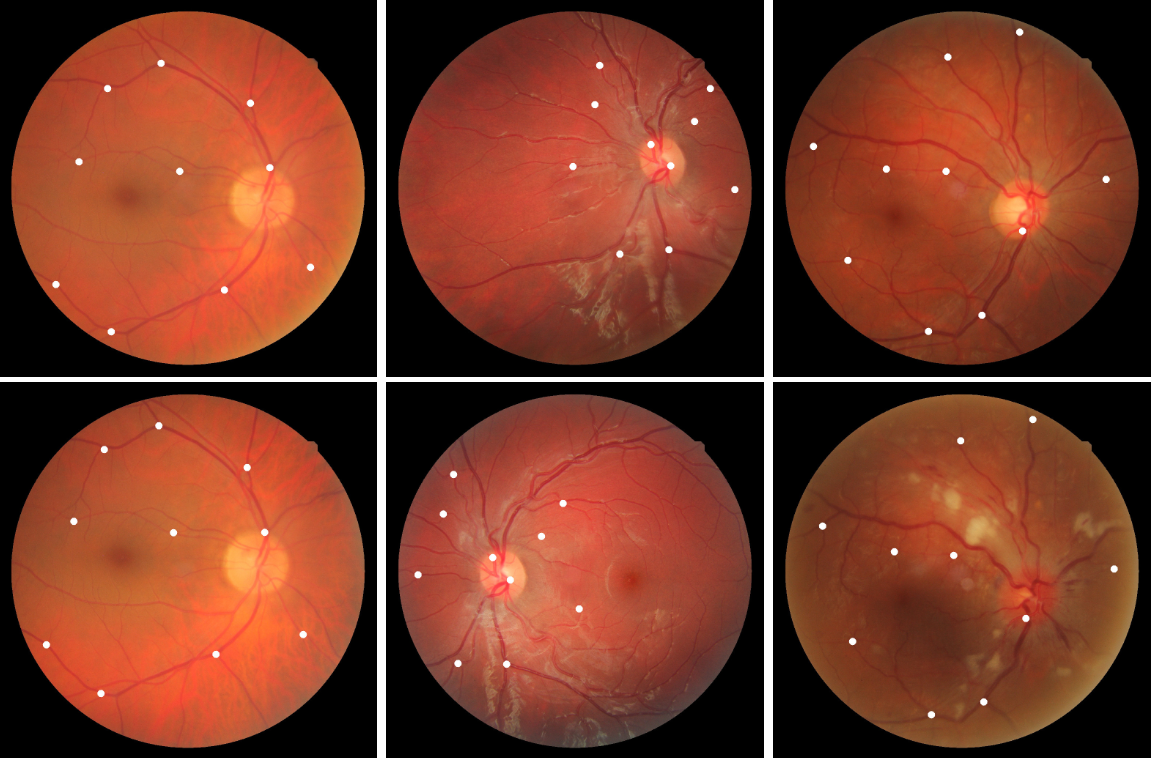
\includegraphics[width=0.8\textwidth]{imaxes/fire-ej.png}
    \caption{Example images from the FIRE dataset \cite{FIRE} with control points indicated. From left to right, categories \textit{\textsf{S}}, \textit{\textsf{P}}, \textit{\textsf{A}}.}
    \label{fig:fire_ej}
\end{figure}

\subsection{RFMID}\label{subsec:RFMID}

The RFMiD dataset \cite{RFMiD} provides 3200 color fundus images with 1712x1712 resolution, labeled according to whether they have any anomaly or not.
It also provides labels for 45 different anomalies annotated by experts.

To use it in this work, we selected a subsample and generated random transformations. We saved the original and transformed images as well as the associated transformation matrices for subsequent evaluation.
It is also divided between color and geometry transformations.

Figure \ref{fig:rfmid_ej} shows an example of an image pair from the RFMiD dataset.

\begin{figure}[tbp]
    \centering
    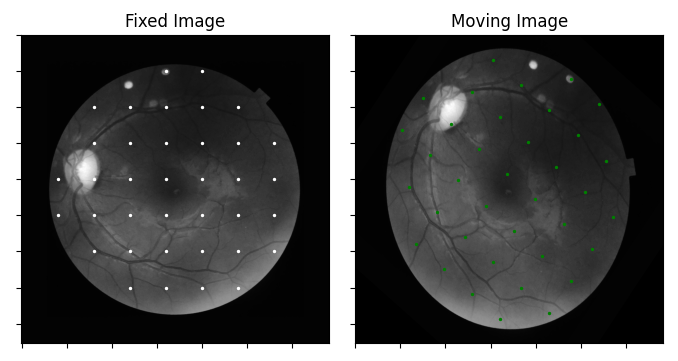
\includegraphics[width=0.8\textwidth]{imaxes/rfmid_ej.png}
    \caption{Example of images from the RFMiD dataset. The image on the left is fixed and the one on the right is moving.}
    \label{fig:rfmid_ej} 
\end{figure} 

\subsection{Differences between datasets}
\label{subsec:Diferencias entre os datasets}

An advantage of using two different datasets is that each has unique characteristics that allow evaluating the model in different contexts.
The main difference is that RMiFD is a synthetic dataset, in which we did not introduce color differences and they always have 100% overlap, so it only evaluates the model's ability to perform geometric registrations.
In contrast, FIRE is a real dataset, in which there are changes in illumination, contrast, overlap and other visual differences, so it evaluates the model's ability to perform registrations under much more adverse conditions.

\section{Experimental Design}
\label{sec:Diseño de Experimentos}

The experimental design is a systematic process that seeks to determine the influence of different factors on a specific outcome. In this case, the objective is to evaluate how different parameters affect the quality of image registration.

Computational cost is a very important factor to consider, since each combination of parameters requires a complete network training for each pair of images, which implies a high energy and time cost.
For example, to test a combination of parameters on FIRE, a network will have to be trained for each pair of images from the 134 in the dataset.
At a training time of 3 minutes per pair, complete training would take more than 6 hours for each parameter combination, with a memory footprint of around 5 GB of VRAM.
The temporal and memory cost depend on several factors, the most relevant being the regularization used, image resolution, batch size and activation function.
Specifically, SIREN has a much higher computational cost than ReLU, requiring about twice the time and memory to train the network.

Due to the large number of factors to consider, a phased experimentation approach was adopted.

Initial experiments were conducted to identify the most promising parameter ranges using a representative subsample of 14 image pairs from each FIRE dataset category, with the objective: Reduce the parameter space for subsequent phases.
In this phase, the loss metric, image resolution, regularization used and batch size were evaluated.

Based on the results of the first phase, more exhaustive experimentation was carried out to try to improve registration performance, focusing on sampling strategy, network weight initialization and dynamic batch size adjustment.

\subsection{Developed Methodologies}
\label{subsec:Metodoloxías Desenvoltas}

For this work, several specific methodologies had to be developed with the aim of improving retinal image registration performance. These methodologies include:

\subsubsection{Sampling Strategies}
\label{subsubsec:estratexias_mostraxe}

\paragraph{Intelligent Sampling}
In the intelligent sampling strategy, a probability mask is calculated for each image, which is used to select the points that are passed to the network. To calculate this mask, blood vessels are extracted using Sobel operators and the optic disc through thresholding. These are the areas where more information is expected, and therefore, they are given higher probabilities of being selected.

\paragraph{Weighted Sampling}
A weighted sampling strategy was also implemented, where random points are selected, but with a higher probability of falling in areas of interest (blood vessels and optic disc), functioning as an intermediate point between random sampling and intelligent sampling.

\paragraph{Uniform Sampling}
A uniform sampling strategy was introduced, where a fixed number of points is selected in each image, ensuring they are uniformly distributed throughout the image. It is a strategy similar to random sampling, but ensuring that as much of the image as possible is covered. This is relevant in experiments with small batch sizes, where random sampling may not cover all areas of the image. To implement it, a Fibonacci lattice-based distribution was used, which allows points to be distributed uniformly over the circular surface of the retina. The position of each point is calculated in polar coordinates, assigning each point a radius proportional to the square root of its index divided by the total number of points, and an angle proportional to the index multiplied by $2\pi$ and divided by the square of the golden ratio ($\varphi^2$):

\[
r_i = \sqrt{\frac{i}{N}}, \quad \theta_i = 2\pi \frac{i}{\varphi^2}
\]
where $i$ is the point index ($i = 1, \dots, N$), $N$ is the total number of points and $\varphi$ is the golden ratio. This way, a uniform and efficient coverage of the region of interest is achieved, avoiding clusters or empty areas.

Figure \ref{fig:sampling_heatmaps} shows the different types of sampling used.

\begin{figure}[tbp]
    \centering
    \begin{subfigure}[b]{0.3\textwidth}
        \centering
        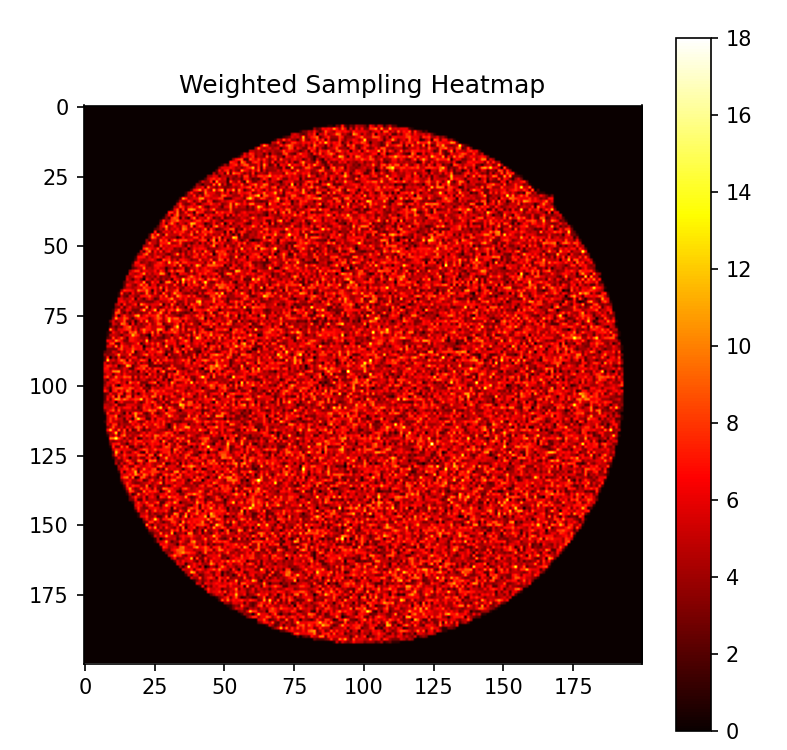
\includegraphics[width=\textwidth]{imaxes/muestraje/random_sampling_heatmap.png}
        \caption{Random sampling heatmap}
        \label{fig:random_sampling_heatmap}
    \end{subfigure}
    \hfill
    \begin{subfigure}[b]{0.3\textwidth}
        \centering
        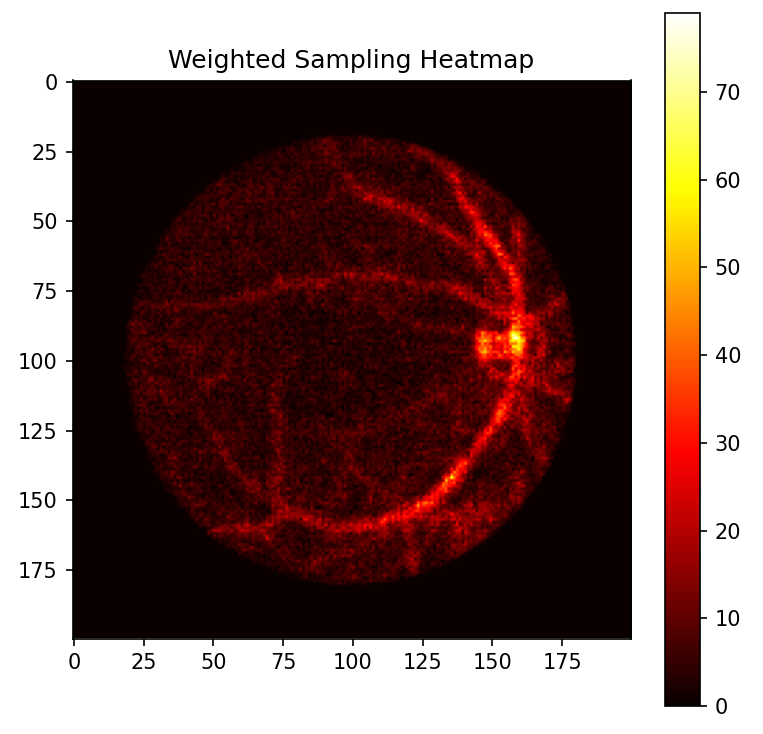
\includegraphics[width=\textwidth]{imaxes/muestraje/weighted_sampling_heatmap.png}
        \caption{Weighted sampling heatmap}
        \label{fig:weighted_sampling_heatmap}
    \end{subfigure}
    \hfill
    \begin{subfigure}[b]{0.3\textwidth}
        \centering
        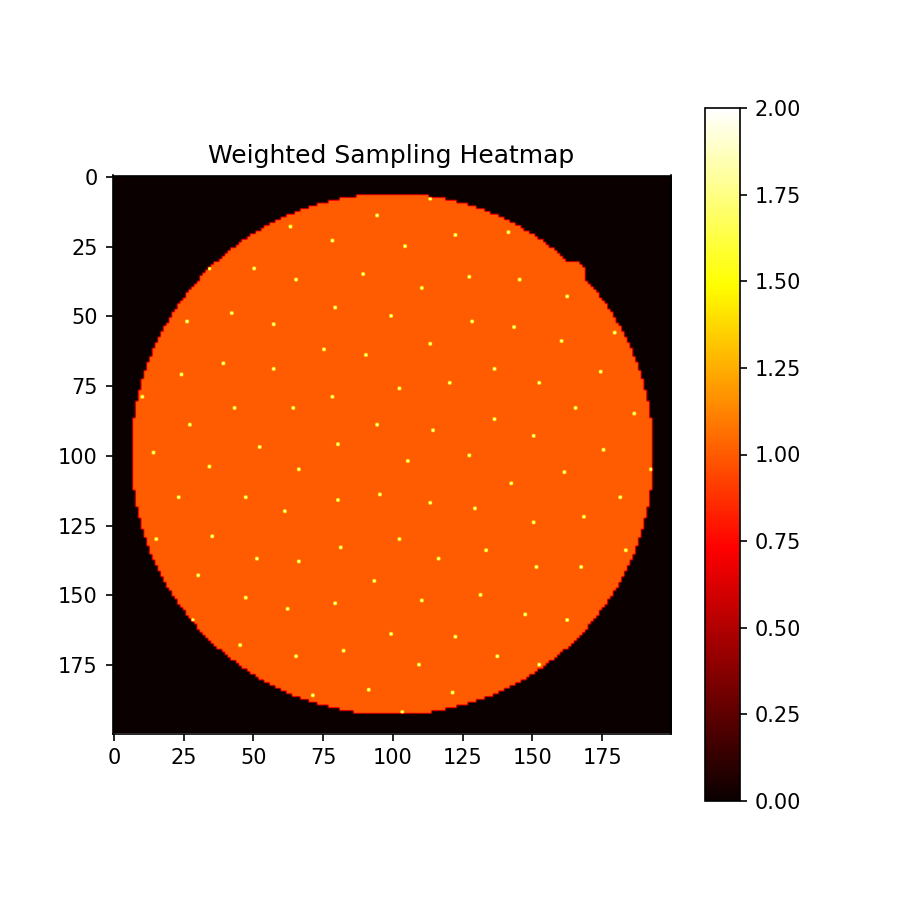
\includegraphics[width=\textwidth]{imaxes/muestraje/uniform_sampling_heatmap.png}
        \caption{Uniform sampling heatmap (100 points)}
        \label{fig:uniform_sampling_heatmap}
    \end{subfigure}
    \caption{Heatmaps illustrating the different sampling strategies implemented.}
    \label{fig:sampling_heatmaps}
\end{figure}

\subsubsection{Initialization Lottery}
\label{subsubsec:loteria_inicializacion}
Another methodology designed was the implementation of the initialization lottery. This technique consists of testing different random initializations of the network weights to determine which ones are most beneficial for convergence and final model performance, and selecting the best initialization to complete training

\subsubsection{Dynamic Batch Size Adjustment}
\label{subsubsec:axuste_dinamico_batch_size}
Dynamic batch size adjustment was implemented, which consists of increasing the number of samples taken by the network throughout training. To carry out this strategy, the epochs are divided into different phases, where each phase uses a different batch size, usually starting with smaller sizes and progressively increasing them.

\section{Evaluation Methods}
\label{sec:Métodos de Avaliación}

The evaluation of registration system performance constitutes a fundamental aspect to determine the effectiveness of the implemented modifications.
The evaluation process is divided into two complementary approaches: quantitative evaluation, which uses objective numerical metrics, and qualitative evaluation, which analyzes results visually to detect artifacts or unwanted deformations that may escape numerical metrics.

Both evaluations are necessary to obtain a complete view of registration quality, as quantitative evaluation may not be sufficient to detect visual problems that are not reflected in the metrics.

\subsection{Quantitative Evaluation}\label{subsec:Avaliación Cuantitativa}

We use as quantitative evaluation method the one proposed by FIRE \cite{FIRE}
generating a graph where the x-axis represents the error threshold value and the y-axis shows the percentage of image pairs that were successfully registered for each error threshold.

The registration error is calculated using the mean Euclidean distance between corresponding points in the fixed and moving images:

\begin{figure}[tbp]
    \centering
    \[
    E = \frac{1}{N} \sum_{i=1}^{N} \left\| p_i^{\text{fixo}} - T(p_i^{\text{móbil}}) \right\|
    \]
    \caption{Registration error calculation using Euclidean distance.}
    \label{fig:erro_registro}
\end{figure}

where N is the number of landmarks, p are the point coordinates and T is the applied transformation.

When the registration error between an image pair is below the threshold, the registration is considered successful and vice versa. This results in a monotonic and continuous curve that reflects the relationship between success rate and target precision, thus avoiding the need to establish an arbitrary threshold.
These graphs are used to illustrate registration accuracy both for individual cases (where the percentage of successfully registered point pairs is used)
and for the complete dataset.
This metric facilitates comparison between different competing methods and allows selecting the most suitable one according to the desired precision.

Additionally, in FIRE the evaluation will be segmented into 3 image categories (S, P and A) to analyze registration performance in each of them, since each category presents different challenges and characteristics.

While FIRE already provides the landmarks for evaluation, RFMID does not.
Therefore, for RFMID, we use the same evaluation method, but generating the points manually so that they cover the interior of the fixed image mask (separated by 50 pixels from each other).

\begin{figure}[tbp]
    \centering
    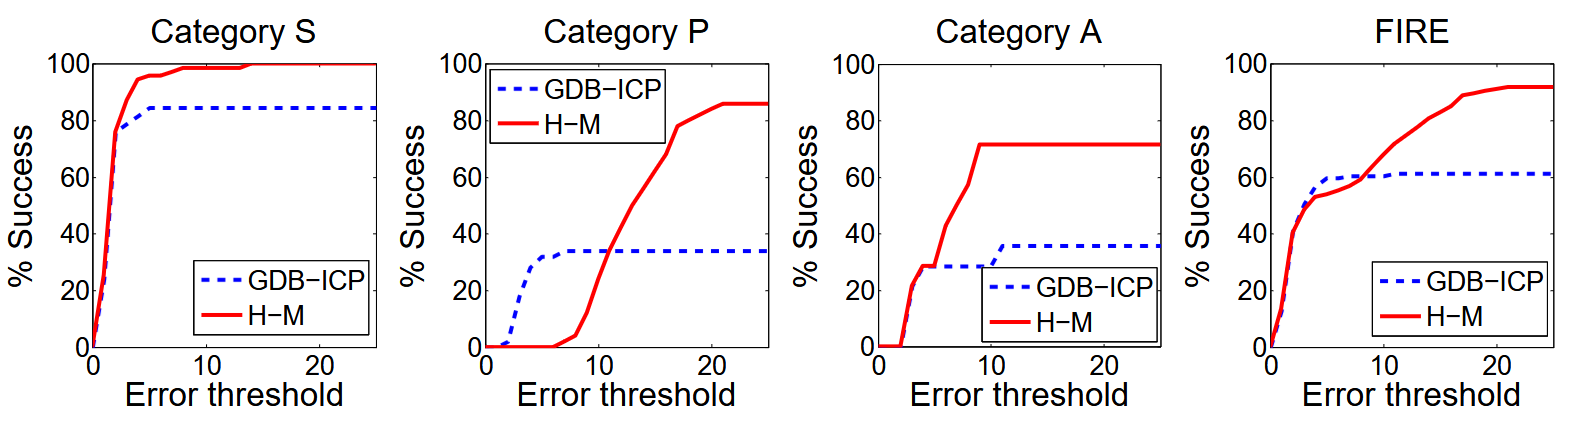
\includegraphics[width=0.8\textwidth]{imaxes/fire_aval.png}
    \caption{FIRE evaluation graph \cite{FIRE}}
    \label{fig:fire_aval}
\end{figure}

In the case of RFMiD, we will divide the dataset into several categories depending on the registration difficulty, which is calculated using the Frobenius norm of a matrix $A \in \mathbb{R}^{m \times n}$.
This is a generalization of the Euclidean distance applied to matrices, where images with larger transformations are considered more difficult.

\begin{figure}[tbp]
    \centering
    \[
    \|A\|_F = \sqrt{\sum_{i=1}^{m} \sum_{j=1}^{n} |a_{ij}|^2}
    \]
    \caption{Frobenius norm of a matrix $A \in \mathbb{R}^{m \times n}$, where $a_{ij}$ are the elements of matrix $A$.}
    \label{fig:frobenius_norm}
\end{figure}

In some cases we will also use the mean distance between corresponding points as a complementary metric to evaluate registration quality, since the success rate may not be sufficient to detect changes.

\subsection{Qualitative Evaluation}
\label{subsec:Avaliación Cualitativa}

In the case of this work, qualitative evaluation becomes very important, since quantitative evaluation only compares a reduced number of points in each image pair.
Visual evaluation allows detecting problems that are not reflected in quantitative metrics, such as visual artifacts or unwanted deformations,
especially in registrations that have local deformations that may not coincide with any point.

In the case of the FIRE dataset \cite{FIRE}, visual evaluation is especially relevant, since only 10 reference points per image are provided, which may not be sufficient to evaluate registration quality in many areas of the image.
Since in RFMID \cite{RFMiD} manually generated reference points are used that cover the entire image, visual evaluation is somewhat less relevant, since it is more likely that an incorrect local deformation will be detected by some point and be reflected in the metrics.

In order to easily identify different visual artifacts or unrealistic transformation, different tools are used such as image composition, displacement vector visualization and comparison of images before and after registration.
Figure \ref{fig:visex} shows some examples of these.

\begin{figure}[tbp]
    \centering
    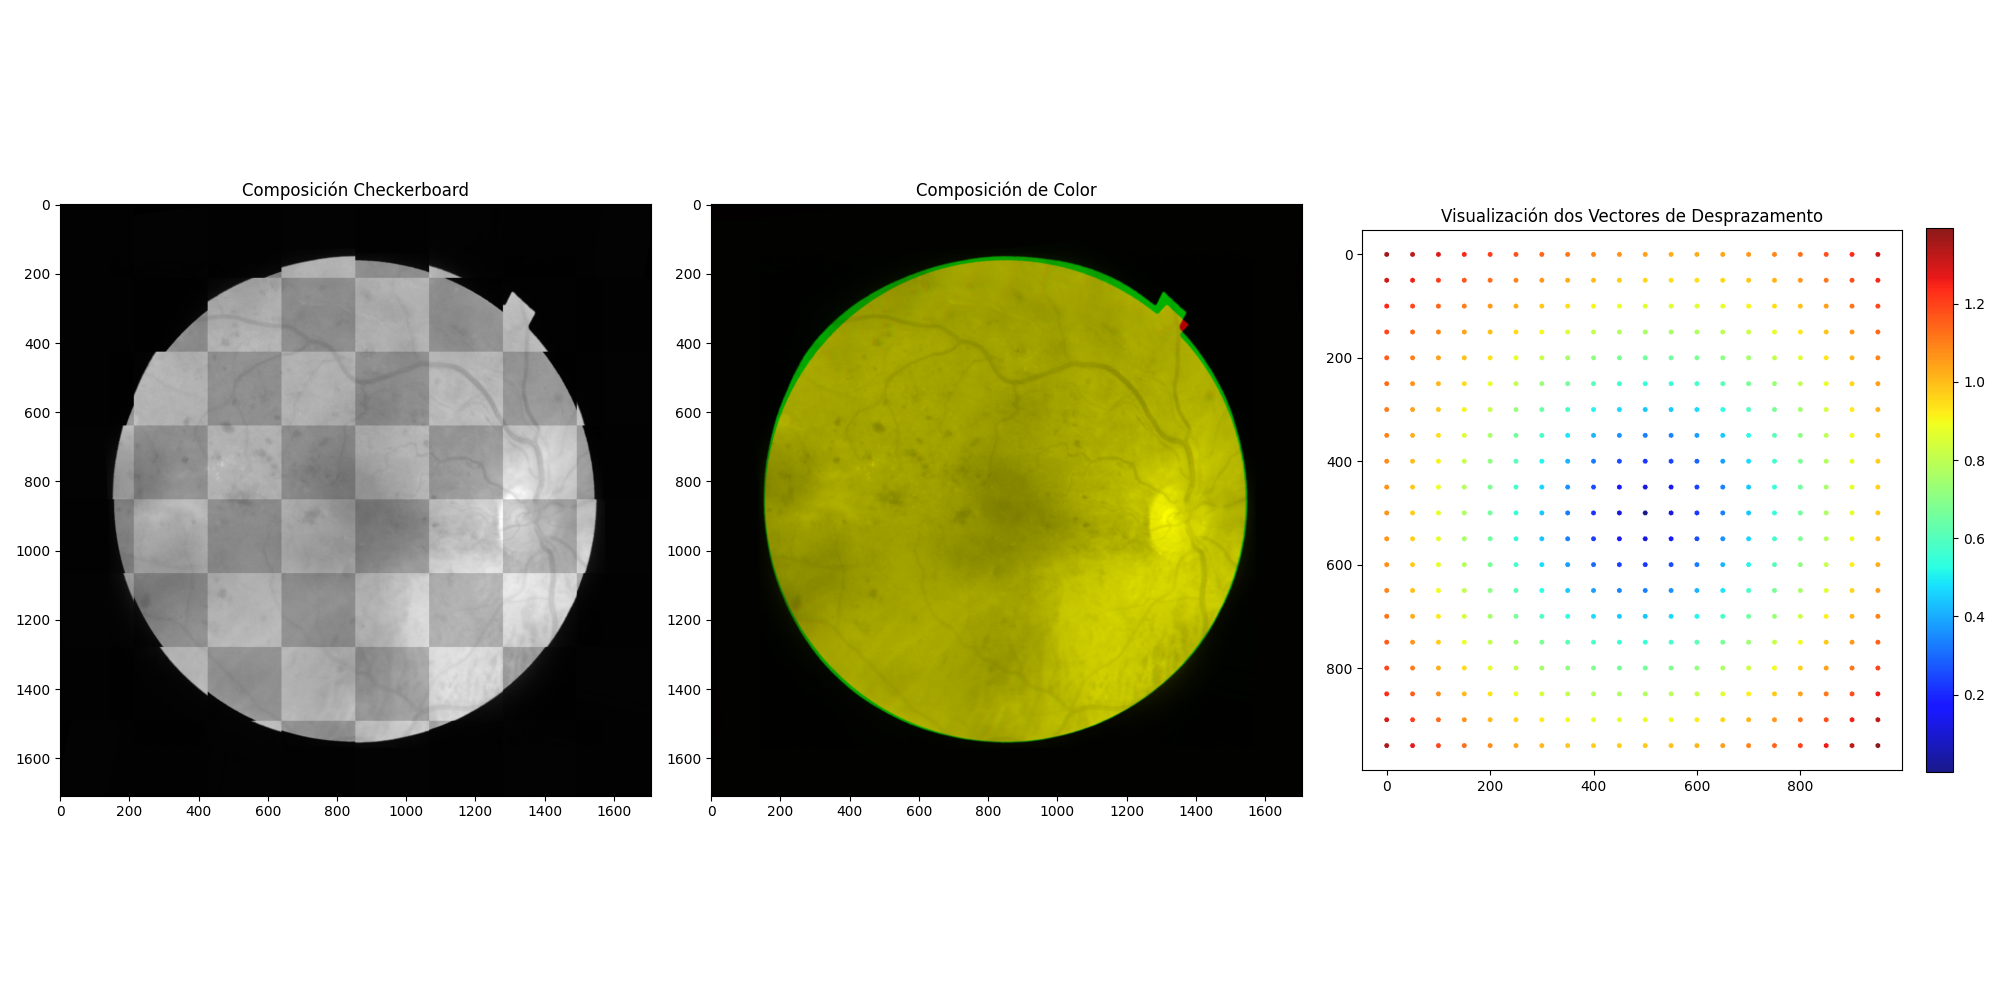
\includegraphics[width=0.9\textwidth]{imaxes/visex.png}
    \caption{Examples of visual evaluation: (a) Checkerboard image composition, (b) Color image composition, (c) Displacement vector visualization.}
    \label{fig:visex}
\end{figure}
 \chapter{Experiments and results}
\label{chap:Experimentos e resultados}
\lettrine{I}{n} this chapter, the experiments carried out and the results obtained will be presented.
To this end, we will begin by presenting an overview of the experimentation process,
followed by the experiments themselves, to finally analyze the results obtained as a whole and the conclusions that can be drawn from them.

\section{Overview}
\label{sec:Vista Xeral}

The objective of this work is to determine if implicit networks are suitable for the retinal registration task. The main comparison focuses on the activation function used (SIREN or ReLU), on the FIRE and RFMID datasets.

The initial evaluation on the FIRE dataset, as can be seen in figures \ref{fig:FIRE_relu} and \ref{fig:FIRE_SIREN}, showed limited performance. Category P proved impossible to register, probably due to the low degree of overlap between images (<75%), while categories S and A barely achieved success rates of 20%.

With the aim of improving this performance and understanding the key factors that influence registration, a series of systematic experiments was designed. This section provides an overview of each of these experiments, advancing their motivation and main findings, which will be detailed in the rest of the chapter.

\begin{itemize}
\item \textbf{Loss function:} The motivation was to find the most robust similarity metric for retinal images, which present great variability in contrast and illumination. The main finding was that the optimal choice depends on the nature of the images: for real images with variability (FIRE), functions based on structural features like NCC offered the best results; for synthetic images without such variability (RFMID), pixel-based functions like L1 were superior.

\item \textbf{Image resolution:} It was investigated whether the high resolution of retinal images (up to 2160x2160) provided a significant benefit compared to the computational cost. The conclusion was that, although very low resolutions were insufficient, no notable improvement was observed above 1250x1250 pixels, establishing this value as a good balance between detail and efficiency.

\item \textbf{Regularization:} This experiment was crucial to avoid unrealistic deformations, a particular risk in SIREN models due to their bias towards high frequencies. It was confirmed that some degree of regularization is indispensable, but the optimal amount of regularization is not universal, rather it depends on the complexity of the transformation.

\item \textbf{Batch size:} Qualitative analysis suggested this was a high-impact parameter. The experiments confirmed it is one of the most critical factors for registration success. A large batch size (e.g., 10000 or more) is fundamental for obtaining good results.

\item \textbf{Sampling strategies:} The initial hypothesis was that prioritizing regions with more information (blood vessels, optic disc) through "intelligent" sampling strategies would improve performance. The results showed that none of the proposed strategies (uniform, weighted) offered a significant advantage over traditional random sampling.

\item \textbf{Initialization:} Given the non-convex nature of the optimization problem, it was explored whether a careful selection of initial weights could improve convergence. An "initialization lottery" was implemented that chooses the best of several initial runs. A marginal but consistent improvement was observed, indicating that initialization has some impact, although it is not a transformative factor.

\item \textbf{Dynamic batch size adjustment:} The strategy of starting with a small batch size to learn the global transformation and then increasing it to refine local details was tested. The result was conclusive and contrary to the hypothesis: this strategy proved to be detrimental, worsening performance. A large and constant batch size from the start proved to be more effective.

\end{itemize}

Unless otherwise specified, for the experiments a learning rate of 0.0001, batch size of 10000 points and 1500 epochs will be used. These values were determined from those originally used by IDIR and from qualitative analysis of results obtained in preliminary experiments. The set of these experiments allows building a detailed understanding of the strengths and weaknesses of implicit networks in this task.

\begin{figure}[tbp]
    \centering
    \begin{subfigure}[b]{0.5\textwidth}
        \centering
        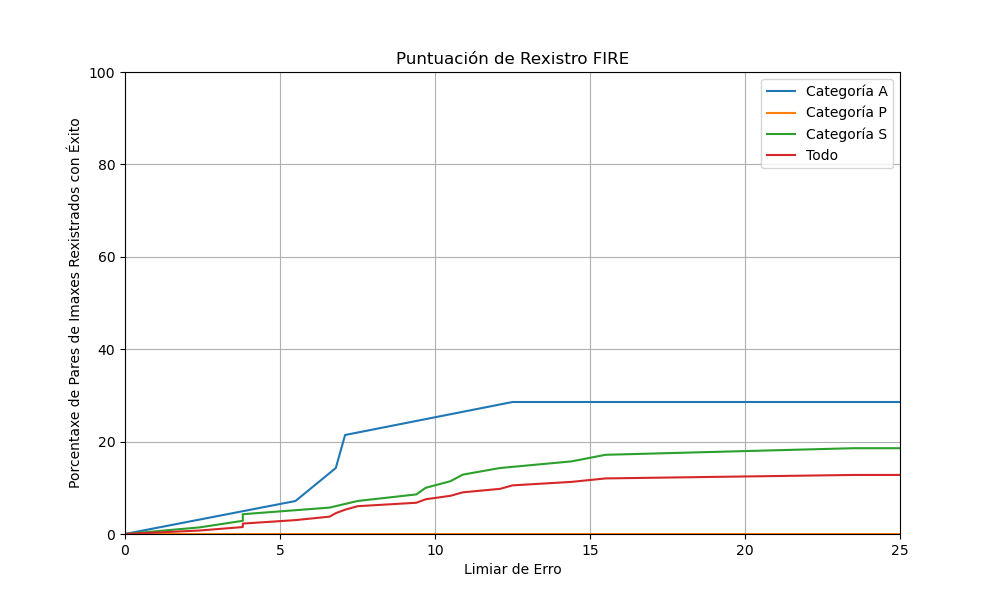
\includegraphics[width=\textwidth]{imaxes/FIRE_scores/fire_registration_score_ReLU.png}
        \caption{FIRE metric, ReLU activation function}
        \label{fig:FIRE_relu}
    \end{subfigure}\hfill
    \begin{subfigure}[b]{0.5\textwidth}
        \centering
        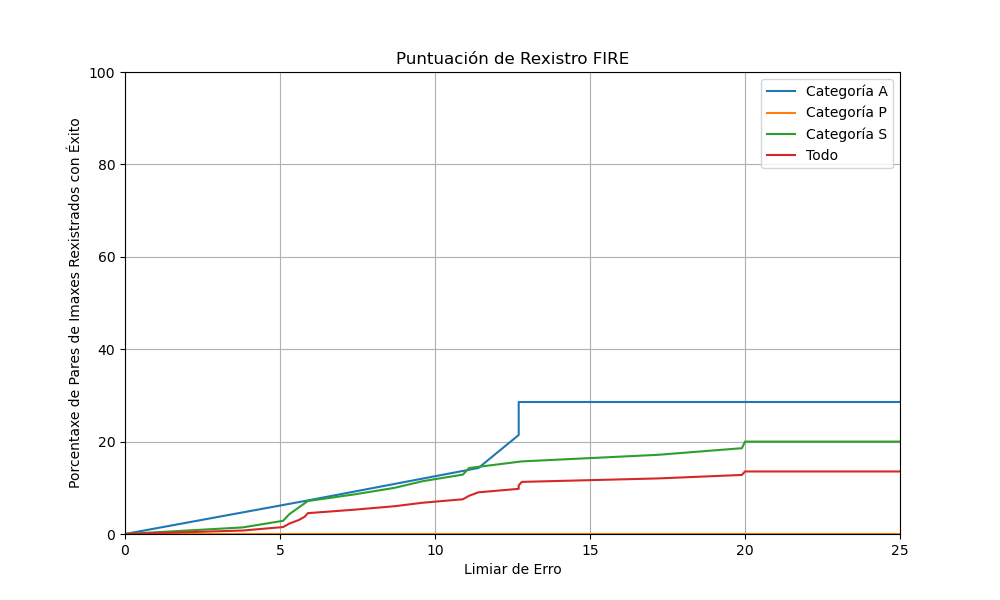
\includegraphics[width=\textwidth]{imaxes/FIRE_scores/fire_registration_scores_SIREN.png}
        \caption{FIRE metric, SIREN activation function}
        \label{fig:FIRE_SIREN}
    \end{subfigure}
    \caption{FIRE dataset metrics}
    \label{fig:FIRE_scores}
\end{figure}

\subsection{Description of experiments}
\label{subsec:Descrición dos experimentos}

\textbf{Initial experiments:} In this part, experiments will be conducted to determine acceptable values for the network parameters in the context of ophthalmological imaging,
as well as determine their influence on network performance.

\begin{itemize}
    \item \textbf{Loss function:} Due to the unique characteristics of retinal images, with variability in illumination and contrast, it is crucial to determine which loss function is more robust for this task. Pixel-based functions (MSE, L1) were compared with structure-based functions (NCC, SSIM) to determine which better captures correspondences between retinal images.
    \item \textbf{Image resolution:} Retinal images can have resolutions up to 2160×2160 pixels, significantly higher than the lung images originally used by IDIR (512×512). It is necessary to determine if higher resolution improves performance or introduces noise that harms registration.
    \item \textbf{Regularization:} SIREN has an inherent bias towards high-frequency signals, which can cause overfitting. The impact of different regularization terms (jacobian, hyperelastic, bending energy) is evaluated to determine the optimal values that avoid unrealistic deformations.
    \item \textbf{Batch size:} The density of points shown to the network can be crucial for registration success. Larger batch sizes provide more information per iteration, but at a higher computational cost. The optimal balance between efficiency and performance is investigated.
\end{itemize}

\textbf{Sampling strategies:} Retinal images have areas with different amounts of structural information (blood vessels, optic disc vs. uniform background). Random, uniform, and content-weighted sampling strategies are compared to determine if prioritizing certain regions improves registration.

\textbf{Initialization:} The non-convex nature of the loss function can cause different initializations to converge to different local minima. An initialization lottery was implemented to select the most promising initialization based on initial loss.

\textbf{Dynamic batch size adjustment:} It is theorized that the network could benefit from first learning global transformations with small batch sizes and then refining with larger amounts of sampled points to capture local details.

\section{Registration examples}\label{sec:Exemplos de rexistro}

Different examples of registration, both successful and failed, can be observed in figure \ref{fig:reg_examples}.
The first image corresponds to the fixed image, the second corresponds to the registered image, the third to the moving image and the fourth to the deformation field applied to a square grid.

The control points can be observed, with white ones being from the fixed image, green ones from the moving image and blue ones displaced by the network.
\begin{figure}[tbp]
    \centering
    \begin{subfigure}[b]{0.45\textwidth}
        \centering
        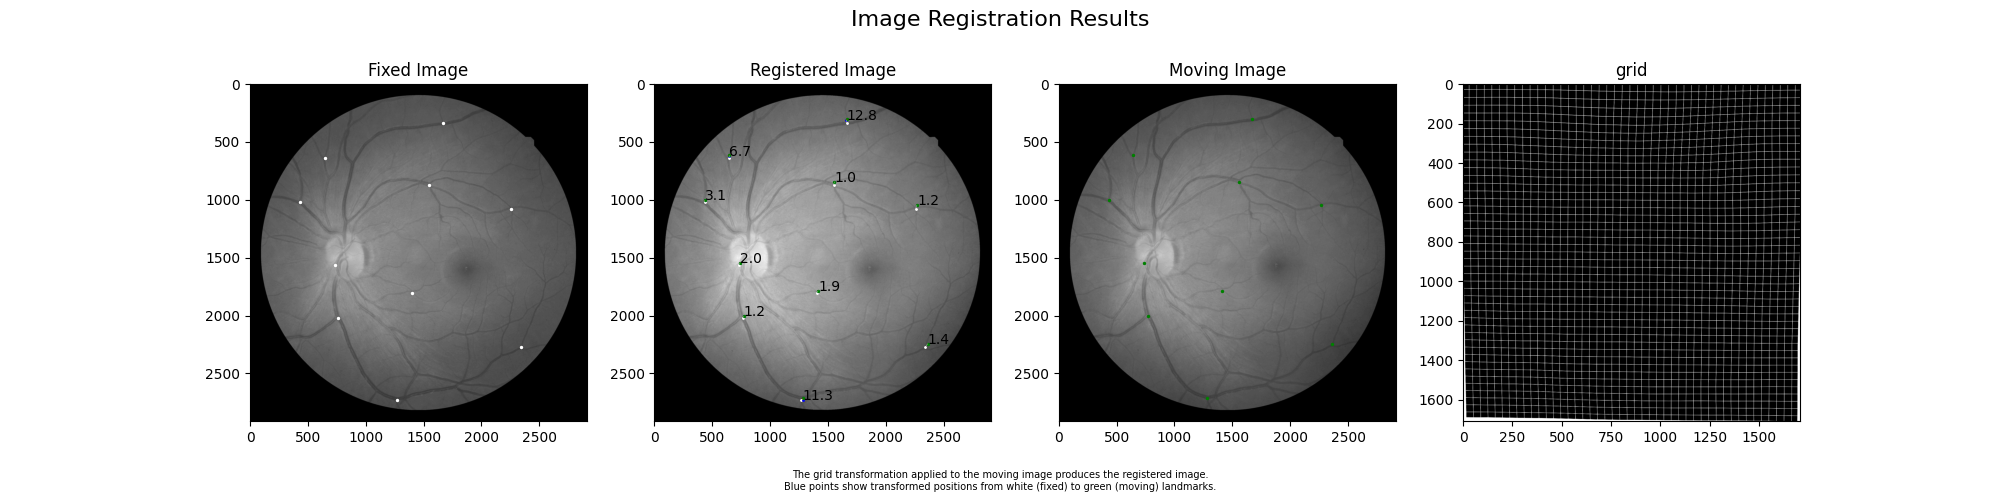
\includegraphics[width=\textwidth]{imaxes/reg_examples/FIRE_MLP_buena.png}
        \caption{Successful registration of an image pair from FIRE dataset with ReLU activation function}
        \label{fig:reg_example_FIRE_MLP_buena}
    \end{subfigure}\hfill
    \begin{subfigure}[b]{0.45\textwidth}
        \centering
        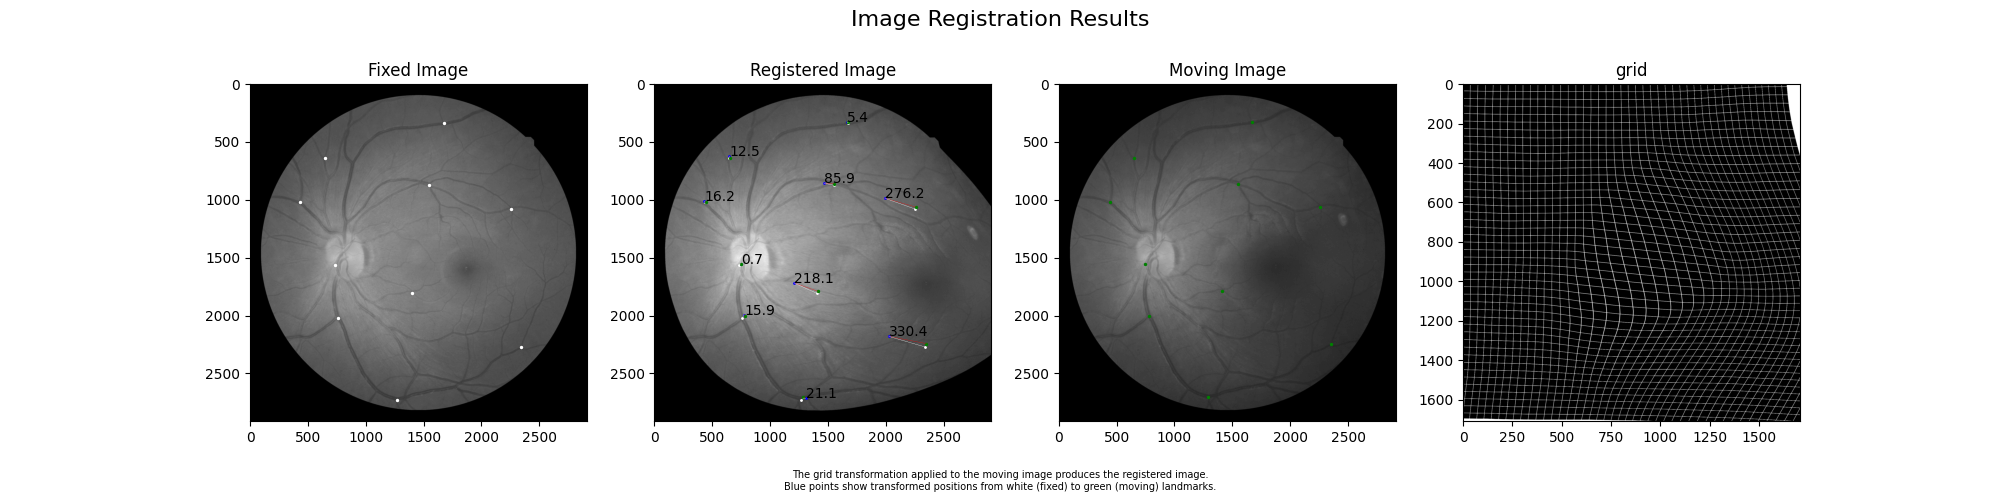
\includegraphics[width=\textwidth]{imaxes/reg_examples/FIRE_MLP_mala.png}
        \caption{Failed registration of an image pair from FIRE dataset with ReLU activation function}
        \label{fig:reg_example_FIRE_MLP_mala}
    \end{subfigure}

    \vskip\baselineskip

    \begin{subfigure}[b]{0.45\textwidth}
        \centering
        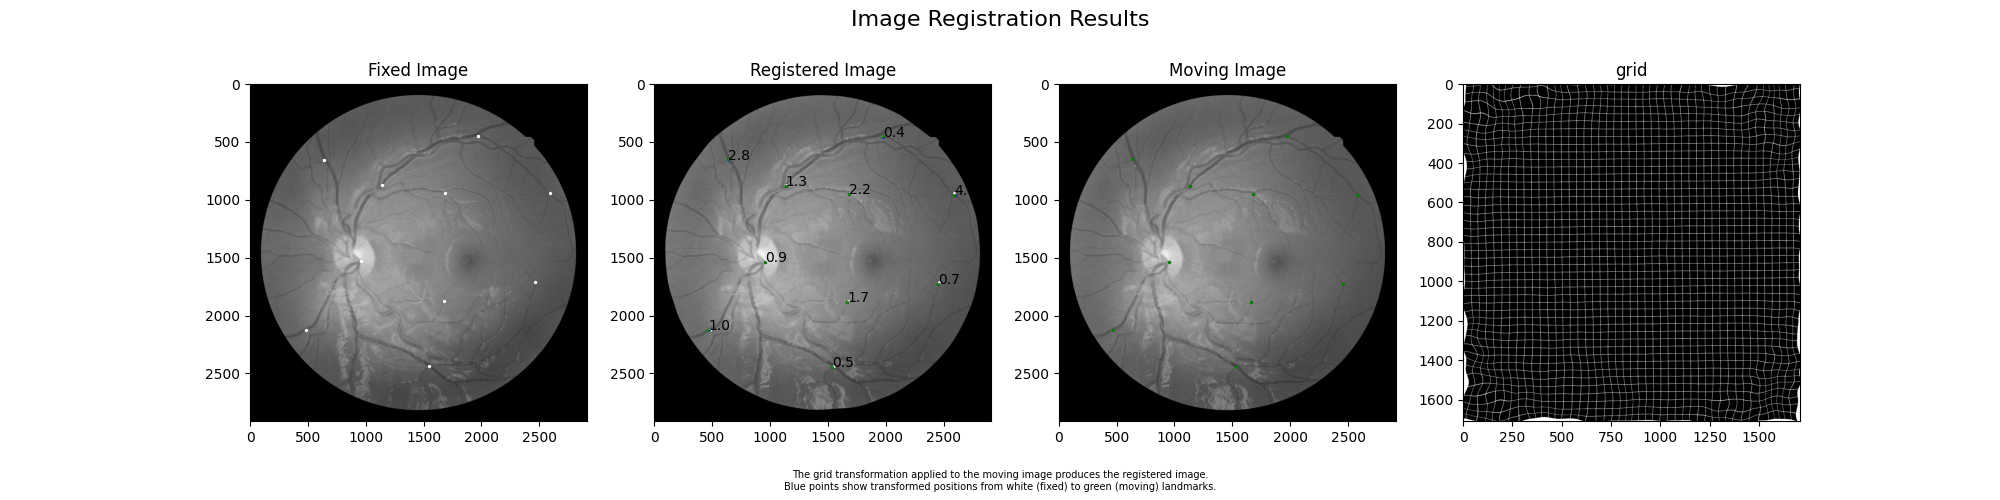
\includegraphics[width=\textwidth]{imaxes/reg_examples/FIRE_SIREN_buena.png}
        \caption{Successful registration of an image pair from FIRE dataset with SIREN activation function}
        \label{fig:reg_example_FIRE_SIREN_buena}
    \end{subfigure}\hfill
    \begin{subfigure}[b]{0.45\textwidth}
        \centering
        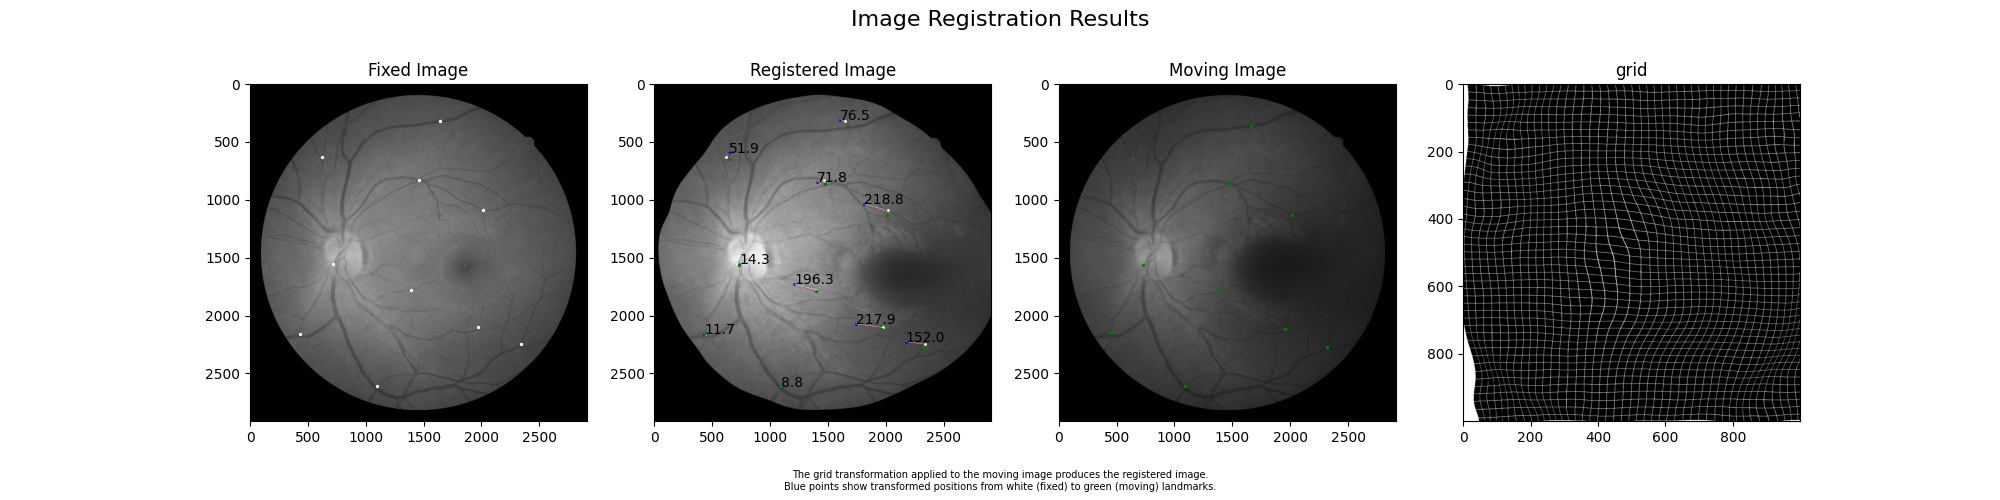
\includegraphics[width=\textwidth]{imaxes/reg_examples/FIRE_SIREN_mala.png}
        \caption{Failed registration of an image pair from FIRE dataset with SIREN activation function}
        \label{fig:reg_example_FIRE_SIREN_mala}
    \end{subfigure}

    \vskip\baselineskip

    \begin{subfigure}[b]{0.45\textwidth}
        \centering
        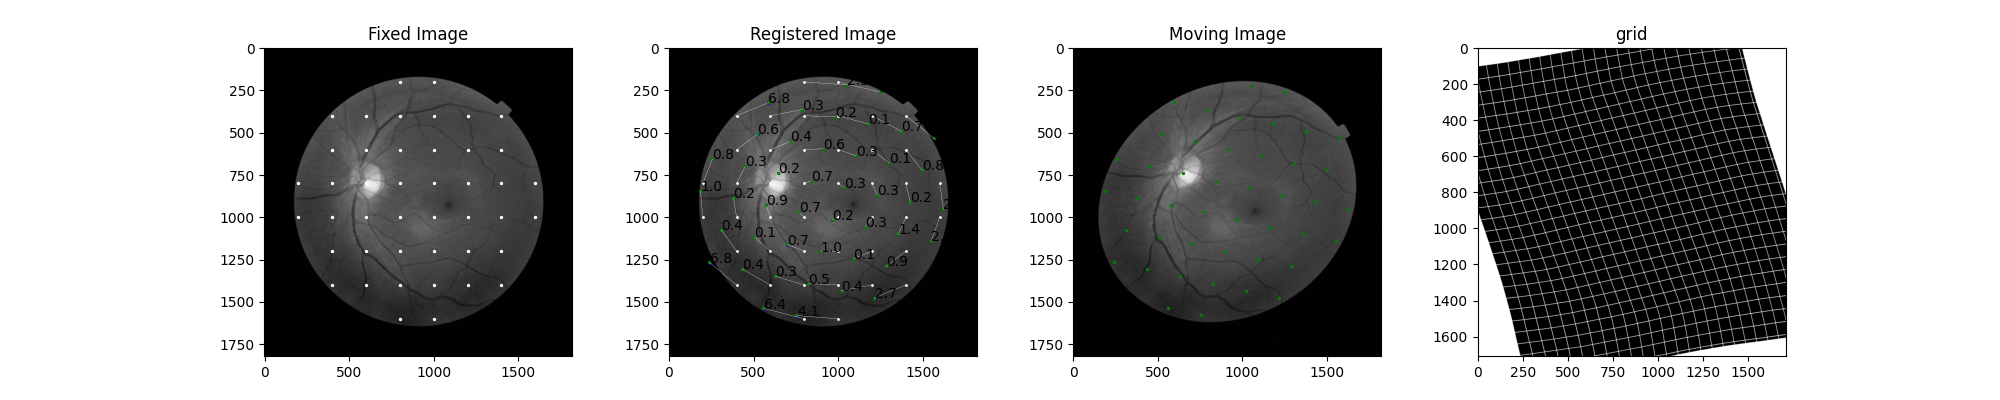
\includegraphics[width=\textwidth]{imaxes/reg_examples/RFMID_MLP_buena.png}
        \caption{Successful registration of an image pair from RFMID dataset with ReLU activation function}
        \label{fig:reg_example_RFMID_MLP_buena}
    \end{subfigure}\hfill
    \begin{subfigure}[b]{0.45\textwidth}
        \centering
        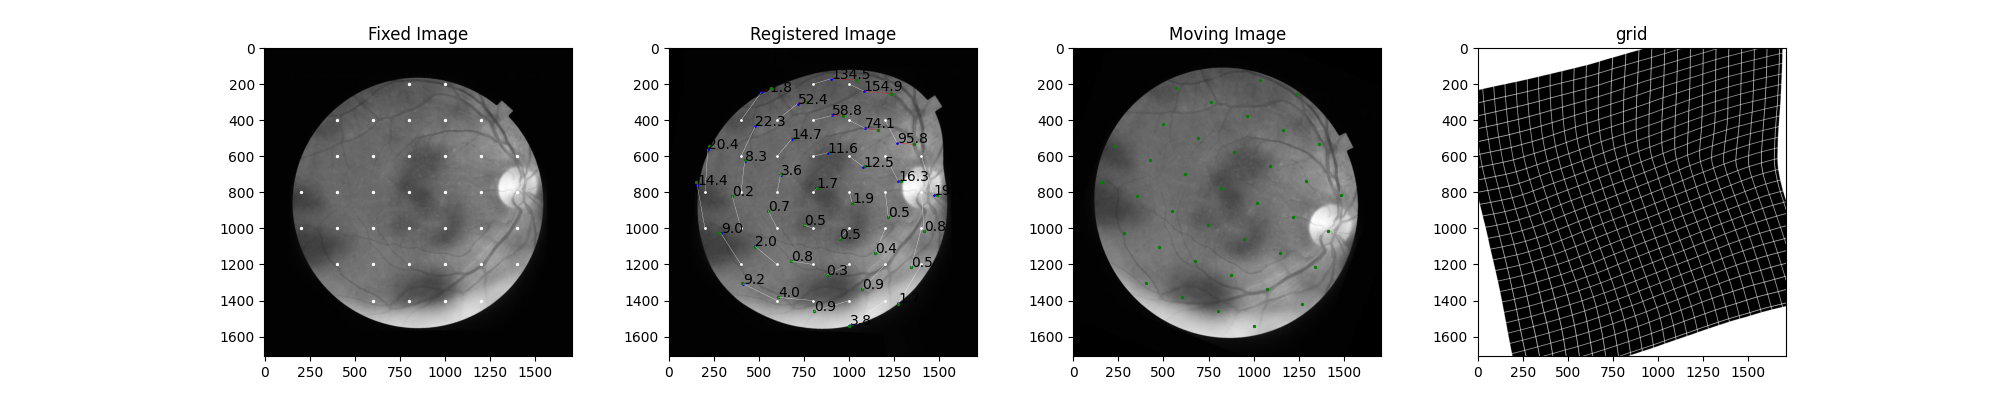
\includegraphics[width=\textwidth]{imaxes/reg_examples/RFMID_MLP_mala.png}
        \caption{Failed registration of an image pair from RFMID dataset with ReLU activation function}
        \label{fig:reg_example_RFMID_MLP_mala}
    \end{subfigure}

    \vskip\baselineskip

    \begin{subfigure}[b]{0.45\textwidth}
        \centering
        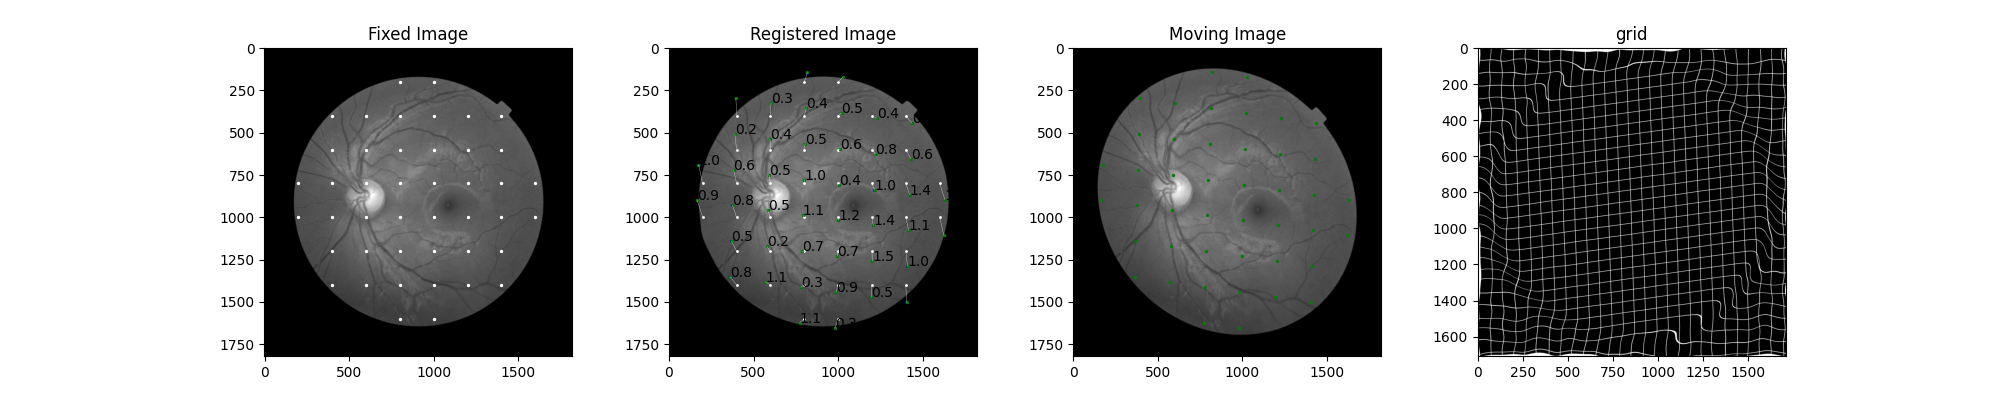
\includegraphics[width=\textwidth]{imaxes/reg_examples/RFMID_SIREN_buena.png}
        \caption{Successful registration of an image pair from RFMID dataset with SIREN activation function}
        \label{fig:reg_example_RFMID_SIREN_buena}
    \end{subfigure}\hfill
    \begin{subfigure}[b]{0.45\textwidth}
        \centering
        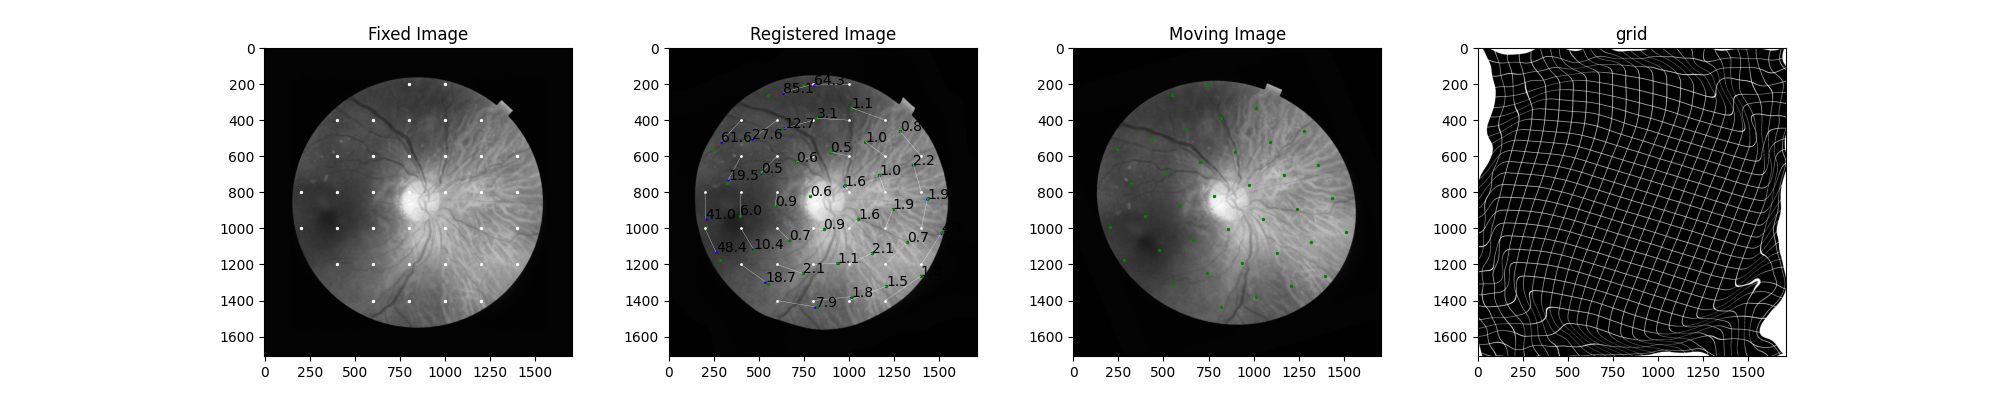
\includegraphics[width=\textwidth]{imaxes/reg_examples/RFMID_SIREN_mala.png}
        \caption{Failed registration of an image pair from RFMID dataset with SIREN activation function}
        \label{fig:reg_example_RFMID_SIREN_mala}
    \end{subfigure}

    \caption{Registration examples: combinations of dataset (FIRE/RFMID), activation function (relu/SIREN) and success.}
    \label{fig:reg_examples}
\end{figure}

\section{Loss Function}
\label{sec:Función de perda}

\subsection{Approach}
\label{subsec:Planteamento-perda}

The loss functions evaluated for this work were already explained in section \ref{subsubsec:Termos de Perda}.

To determine which loss function is most suitable for the retinal registration task, experiments were conducted comparing the performance of each one on a sample of images from the FIRE and RFMID datasets.
Since the network is not able to successfully register a large portion of the images under these conditions, the average distance of all points will be taken as a comparison metric.

\subsection{Results}
\label{subsec:Resultados-perda}

The comparison between different loss functions is presented in figure \ref{fig:loss_functions_comparison}.

\begin{figure}[tbp]
    \centering
    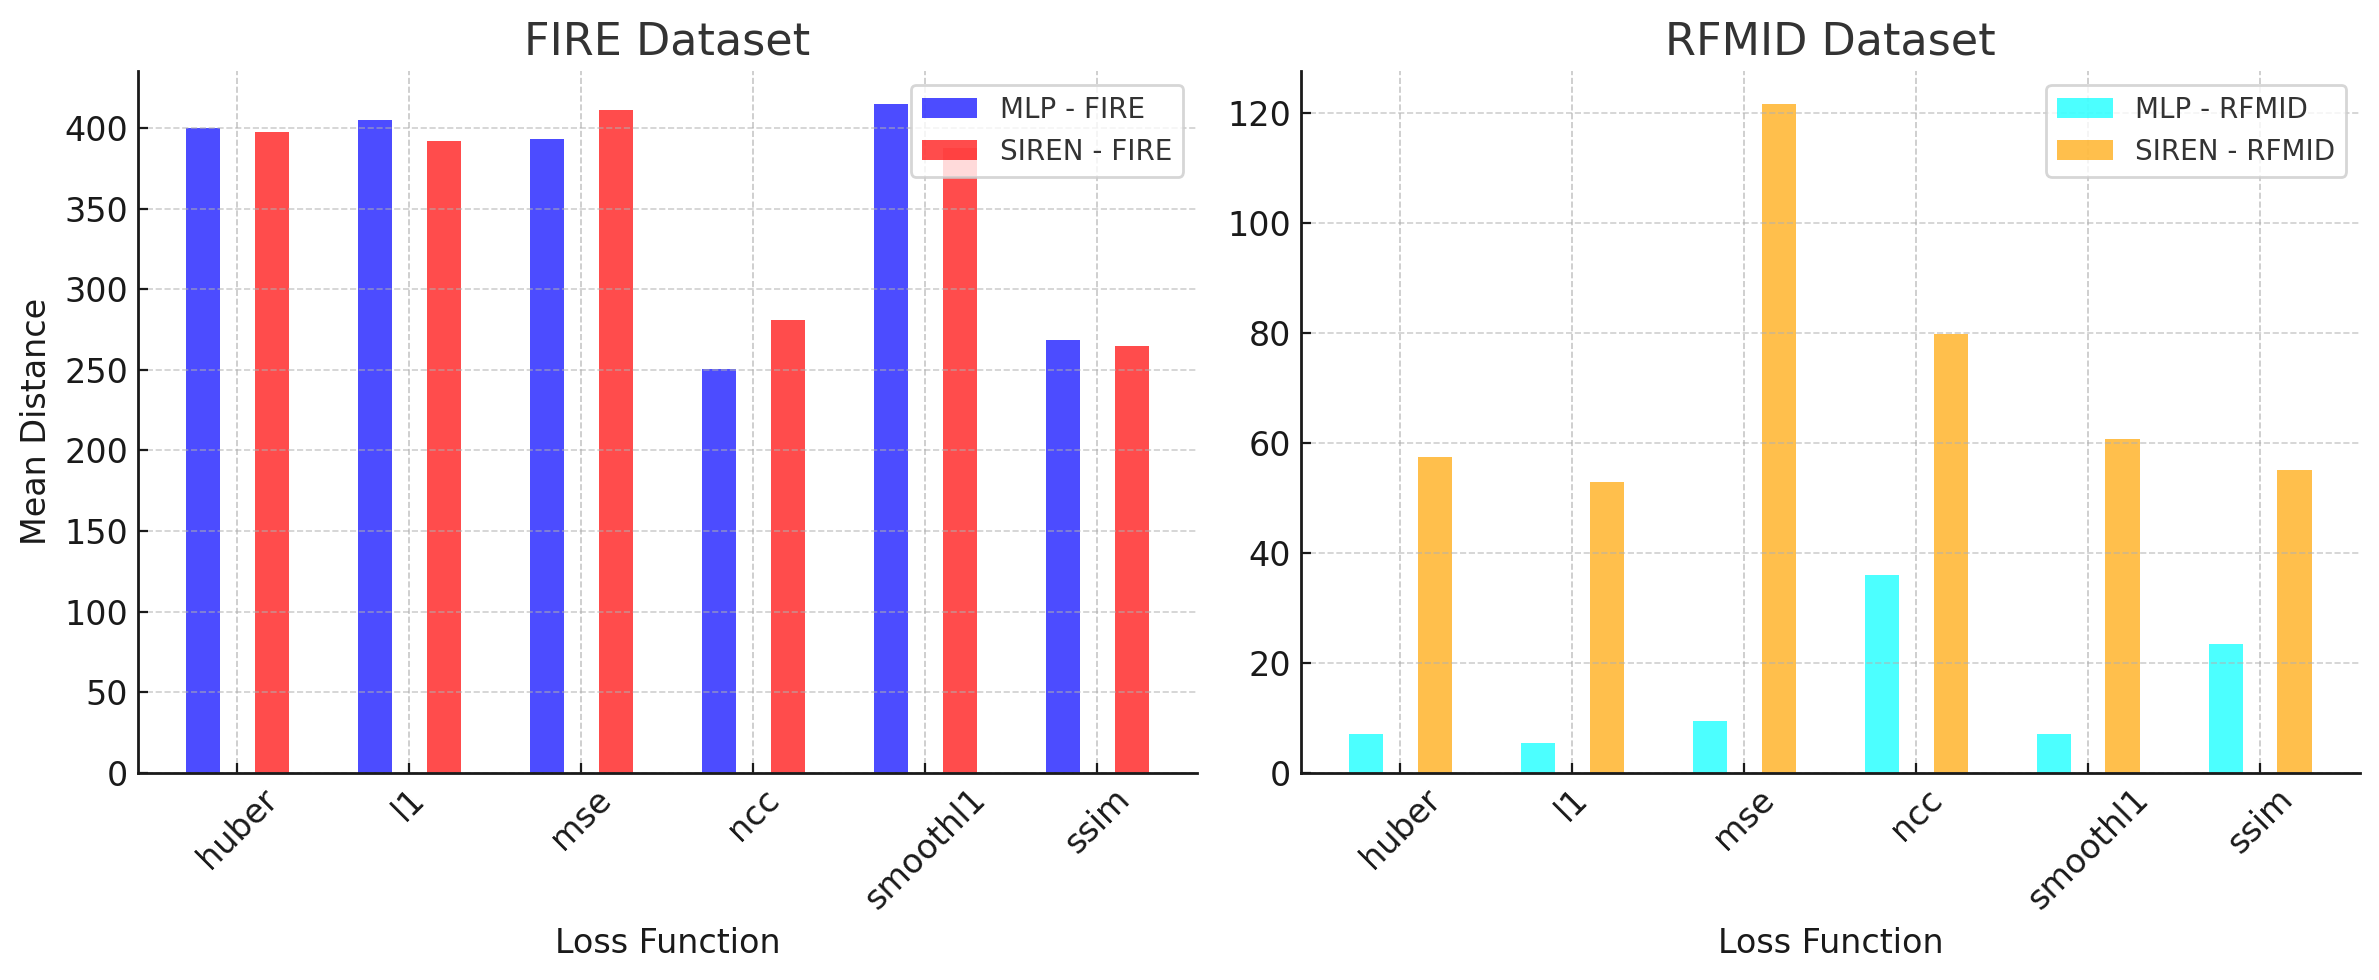
\includegraphics[width=1\textwidth]{imaxes/losstype.png}
    \caption{Comparison of different loss functions on FIRE and RFMID images}
    \label{fig:loss_functions_comparison}
\end{figure}

\subsection{Discussion}
\label{subsec:Discusion-loss}

It is observed that metrics that take into account image structure (NCC, SSIM) tend to give better results than those that don't (MSE, Huber, Smooth L1) with the FIRE dataset, while with RFMID the opposite occurs.
This may be due to real retinal images having greater variability in illumination and contrast, so metrics that don't take into account image structure will be less robust to these differences.
In the case of RFMID, being synthetic images, the variability in illumination and contrast is null, which explains the better results of metrics that don't take into account image structure.
Similarly, the Relu activation function tends to produce predominantly linear functions, which better adapts to the transformations made in the RFMID dataset.

SSIM is less robust to noise and sensitive to the size of sections used, as well as computationally expensive. Additionally, it has another added cost since it's not possible to calculate SSIM just by comparing the shown points as it uses sliding windows to evaluate luminance, contrast and structure.
To use it, it's necessary to reconstruct the image in each iteration which has a high computational cost.
In case of not reconstructing the image and using the shown points directly, this metric works equally but with slightly worse results, as it loses all its ability to capture local variations in luminance, contrast and structure, which translates into a global loss function without local considerations.

\subsection{Conclusions}
\label{subsec:Conclusions-loss}

Based on the obtained results, the following conclusions can be drawn:
\begin{itemize}
    \item For the FIRE dataset, which contains real retinal images with variability in illumination and contrast, loss functions based on structural features like NCC and SSIM provide significantly better results.
    \item For the RFMID dataset, which contains images with only geometric variation, pixel-based loss functions like L1 and Huber offer better results.
    \item A systematic difference is observed between Relu and SIREN models, with the former being more effective for the RFMID dataset, while both show comparable performance for FIRE.
\end{itemize}

\section{Image Resolution}
\label{sec:Resolución da imaxe}

\subsection{Approach}
\label{subsec:Planteamento-resolution}

To determine which resolution is most appropriate, experiments were conducted comparing the performance of each one on a sample of images from the FIRE and RFMID datasets.
Since the network is not able to successfully register a large portion of the images, the average distance of all points will be taken as a comparison metric.

Image resolution directly influences the rest of the network parameters.
For example, a batch size of 1000 points in a 256x256 image is a much higher point density than in a 1024x1024 image.

Additionally, image resolution also influences the network's ability to learn transformations, as it receives more detailed information.
This can be beneficial if these details contain relevant information for the registration task, but it could also be detrimental if they contain a large amount of noise.

Image size is also one of the main differences between retinal images and lung images originally used by IDIR, with the latter being 512x512 while eye images have resolutions of up to 2160x2160.

\subsection{Results}\label{subsec:Resultados-resolution}

The comparison between different resolutions is presented in figure \ref{fig:resoluciónchart}.

\begin{figure}[tbp]
    \centering
    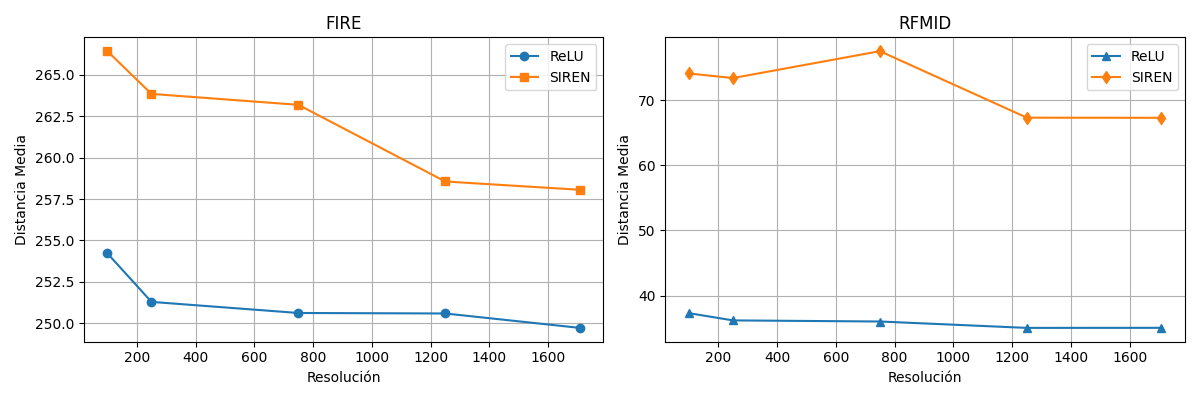
\includegraphics[width=1\textwidth]{imaxes/resolutionchart.png}
    \caption{Comparison of different loss resolutions on FIRE and RFMID images. Lower mean distance is better.}
    \label{fig:resoluciónchart}
\end{figure}

\subsection{Discussion}
\label{subsec:Discusion-resolution}

It can be observed that a higher resolution tends to give slightly better results, but at a higher computational cost.
This may be due to the precision of the evaluation rather than a better ability of the network to learn the transformations, since the differences are very small and consistent between different pairs of images.
This suggests that resolution does not have a significant impact on network performance, and that most of the relevant information for the registration task is already captured at lower resolutions.

\subsection{Conclusions}
\label{subsec:Conclusions-resolution}

Based on the obtained results, we can conclude that:

1. Resolutions below 100×100 do not capture enough details of retinal vascular structures to perform accurate registration, especially in real images from the FIRE dataset.

2. Increasing resolution above 1250x1250 does not provide significant benefits.

For subsequent experiments, a standard resolution of 1250x1250 pixels will be adopted, which has proven to provide a good balance between performance and computational efficiency.

\section{Regularization}
\label{sec:Regularización}

\subsection{Approach}
\label{subsec:Planteamento-regularization}

To determine the optimal amount of regularization, experiments were conducted comparing the performance of each one on a sample of images from the FIRE and RFMID datasets with different activation functions and different degrees of regularization.

The regularization process helps the network avoid overfitting by modifying the loss term to penalize unrealistic transformations.
The regularization techniques evaluated, which were already explained in detail in section \ref{subsubsec:Termos de regularización}

The values used for each type of regularization were adjusted from those originally used by IDIR and compared the impact of each of them on the loss function, since the scale of each of them is different.

Annex \ref{sec:Anexo regularization} details a more complete search to explore the relationships between different types of regularization.
This section will only present the results of experiments conducted with hyperelastic regularization, which is considered the most relevant for this task.

\subsection{Results}
\label{subsec:Resultados-regularization}

The comparison between different hyperelastic regularization values is presented in figure \ref{fig:barplot_hyper_reg_comparison}.

\begin{figure}[tbp]
    \centering
    \begin{subfigure}[b]{0.48\textwidth}
        \centering
        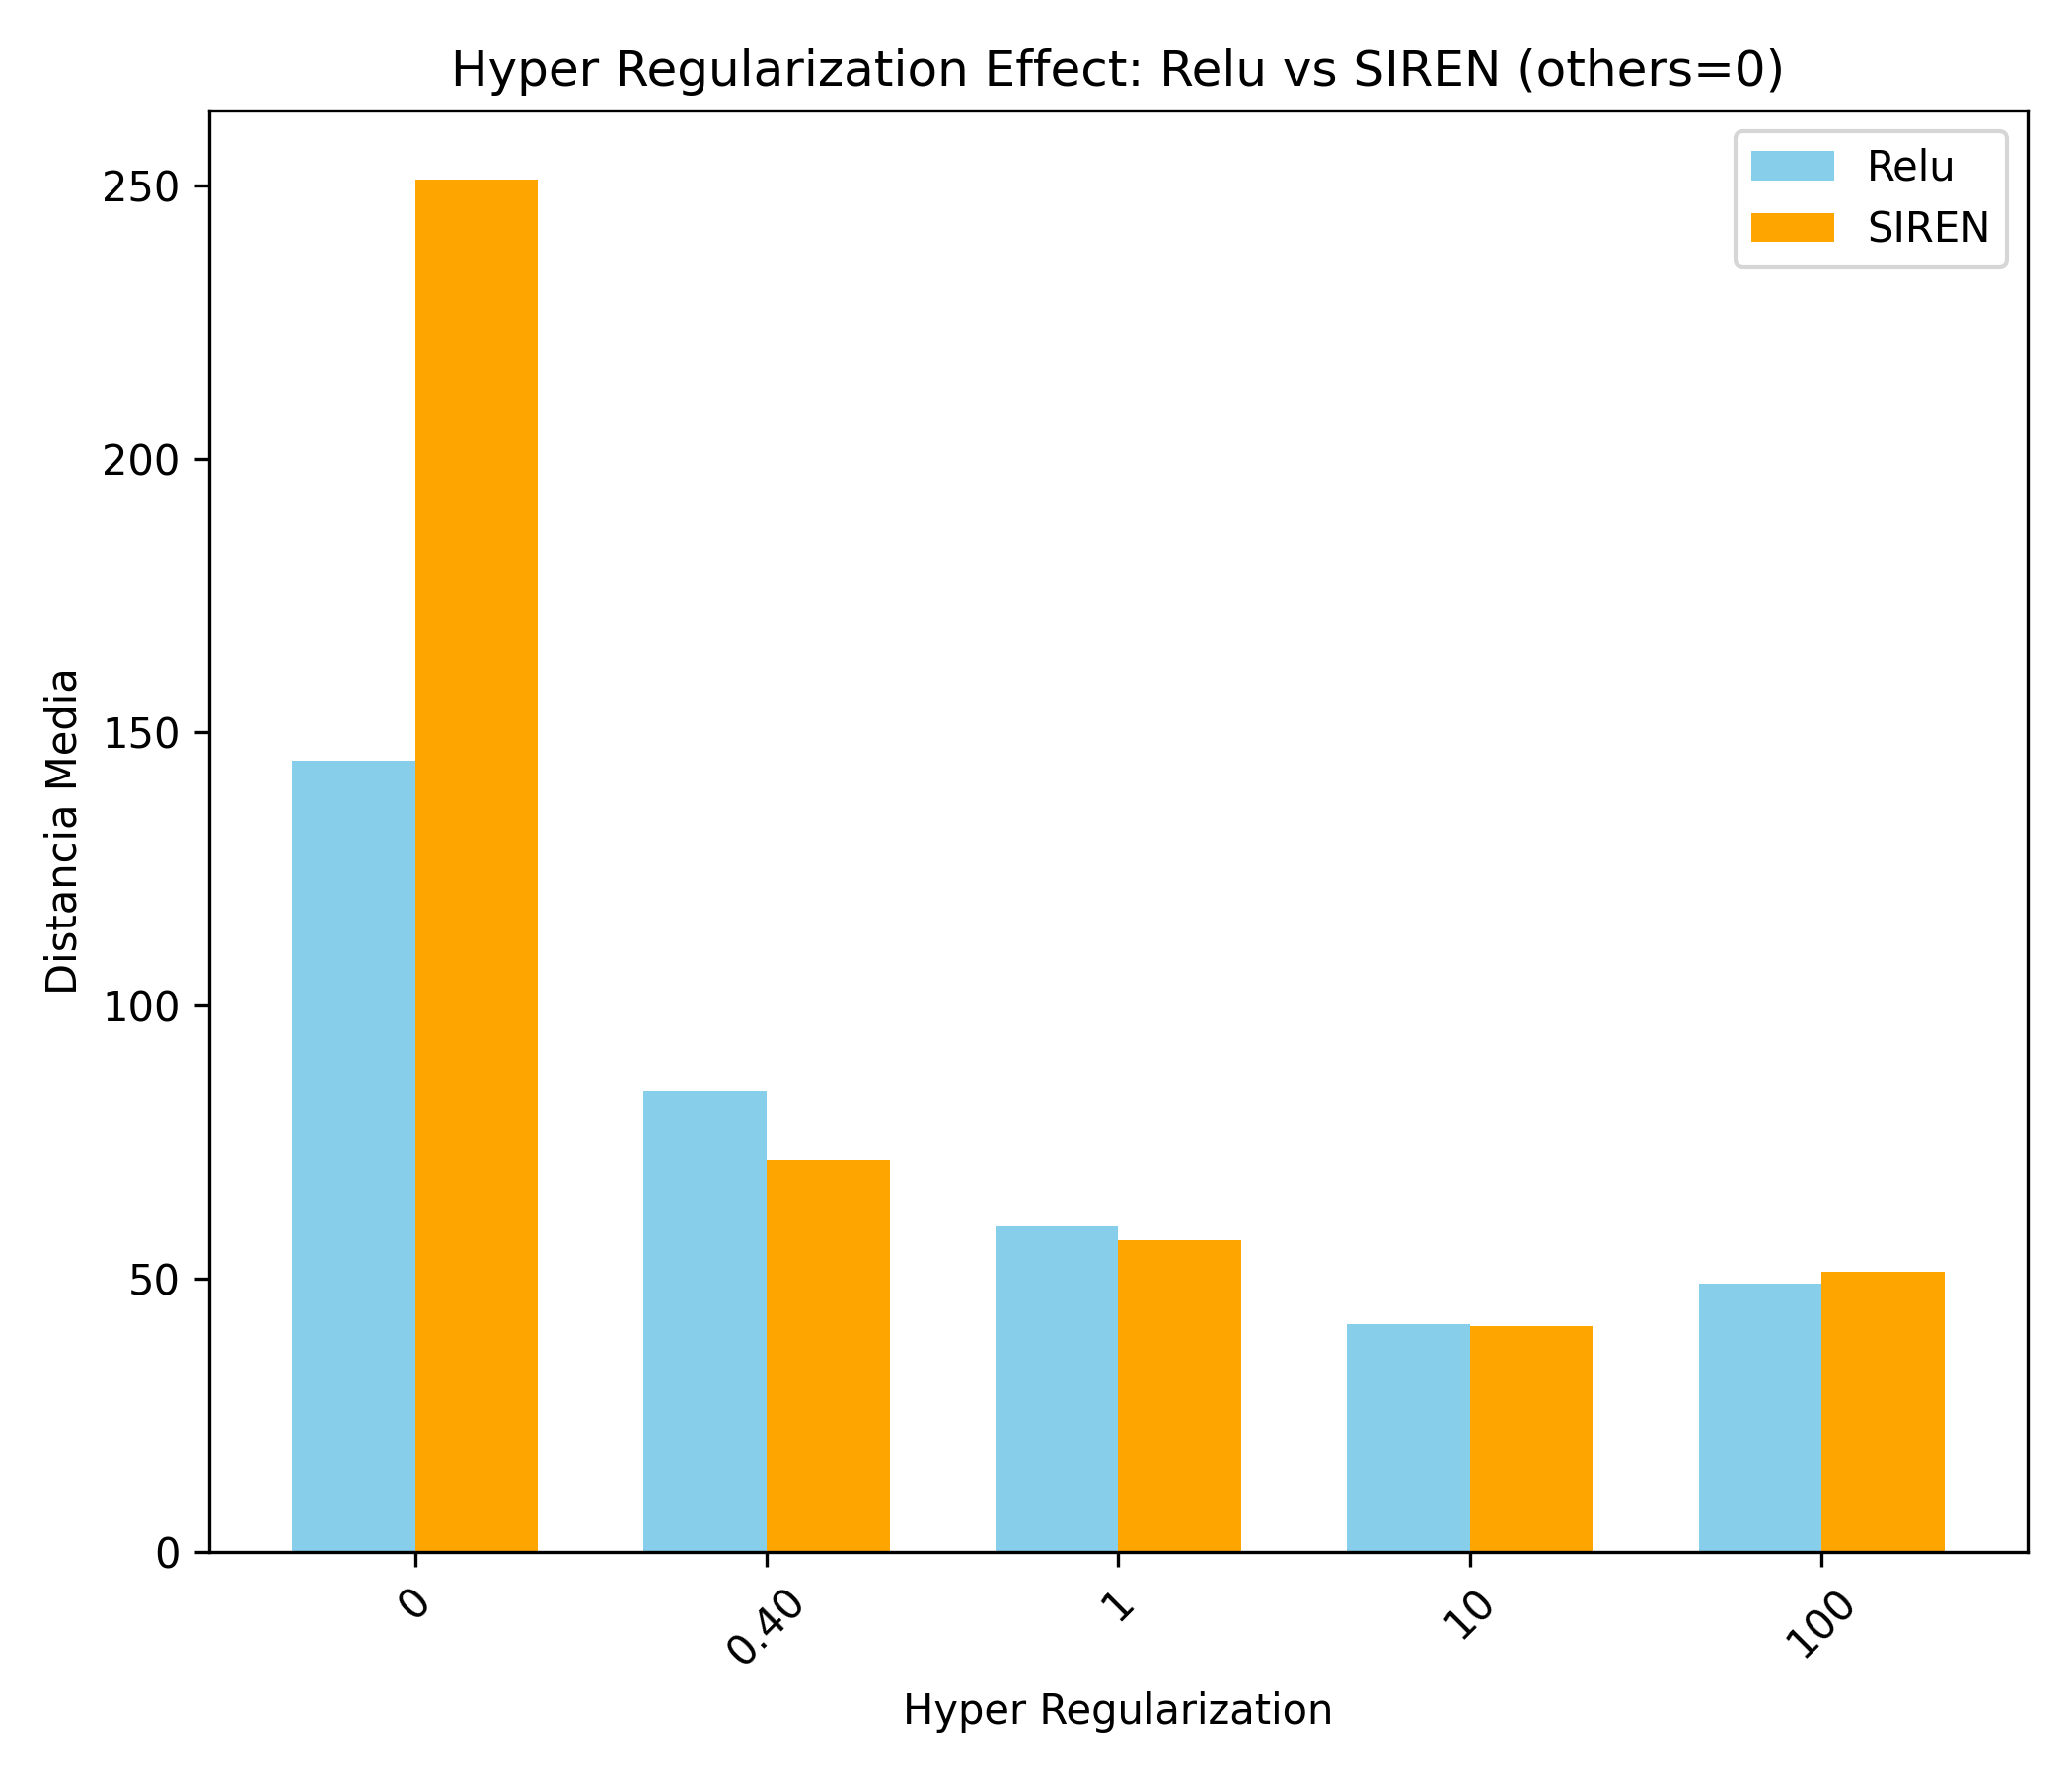
\includegraphics[width=\textwidth]{imaxes/reg_examples/barplot_hyper_reg_comparison_MLP_vs_SIREN_FIRE.png}
        \caption{Comparison of hyperelastic regularization in FIRE}
        \label{fig:barplot_hyper_reg_comparison_MLP_vs_SIREN_FIRE}
    \end{subfigure}\hfill
    \begin{subfigure}[b]{0.48\textwidth}
        \centering
        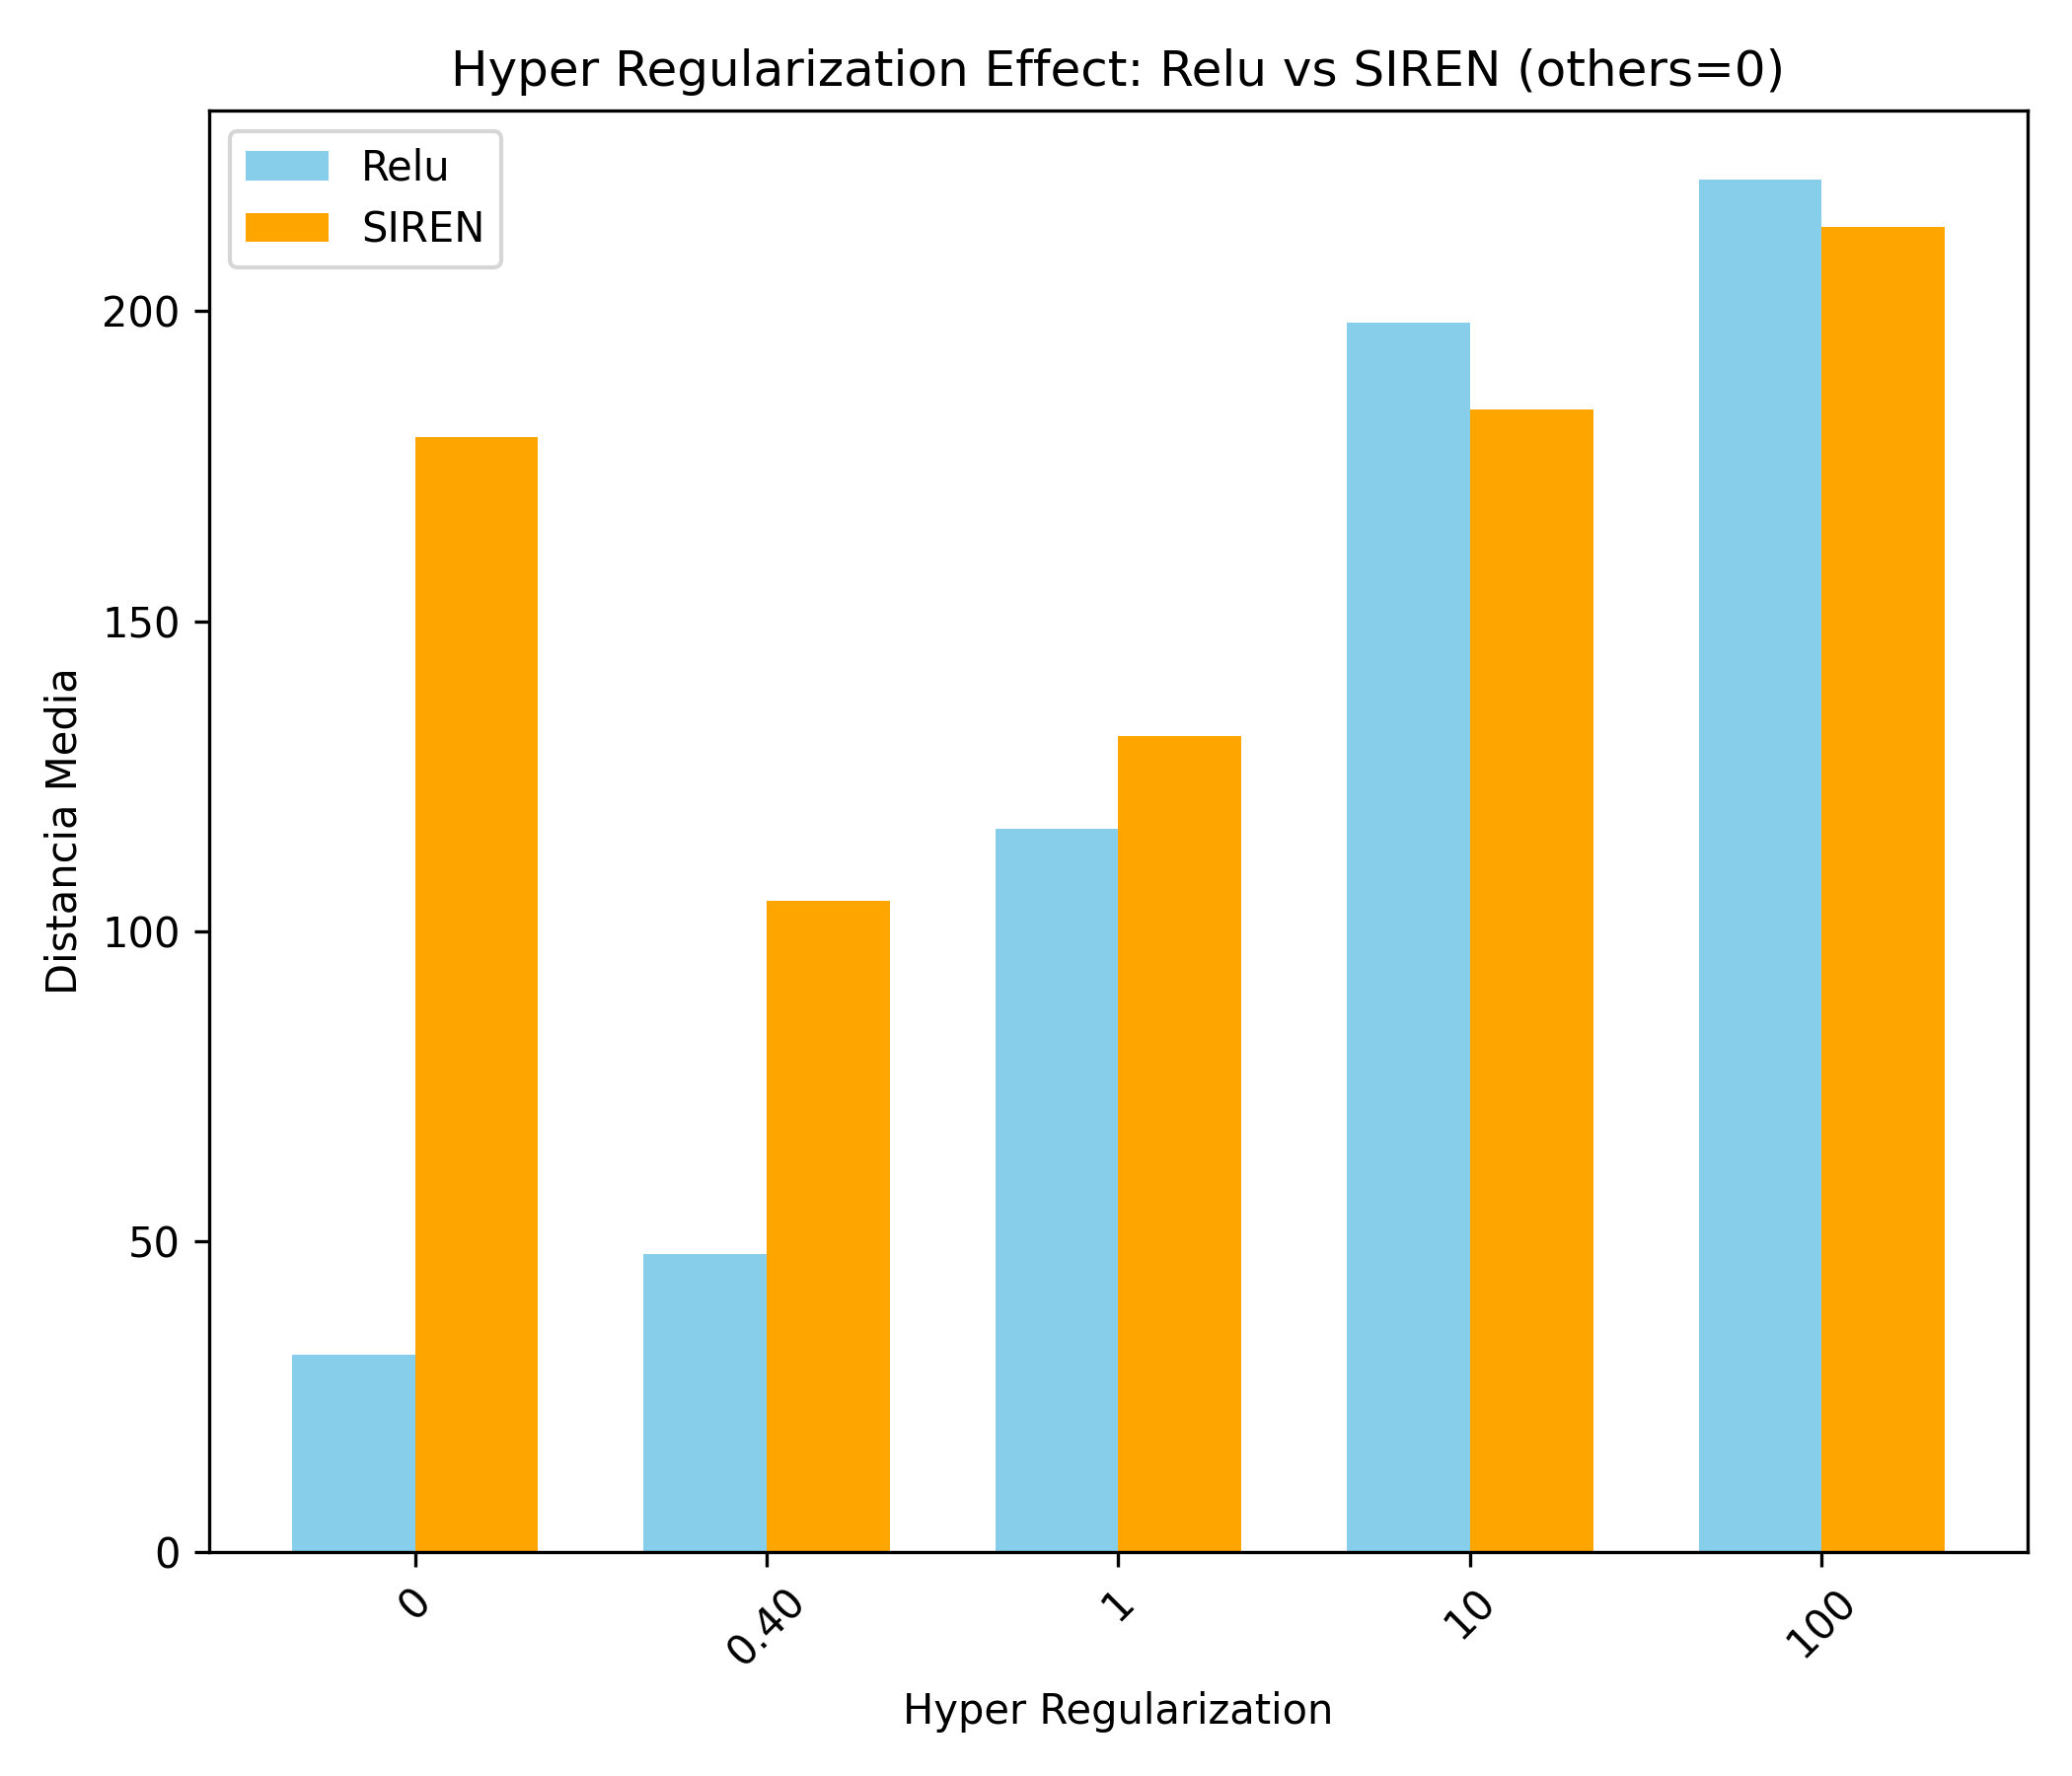
\includegraphics[width=\textwidth]{imaxes/reg_examples/barplot_hyper_reg_comparison_MLP_vs_SIREN_RFMID.png}
        \caption{Comparison of hyperelastic regularization in RFMID}
        \label{fig:barplot_hyper_reg_comparison_MLP_vs_SIREN_RFMID}
    \end{subfigure}
    \caption{Comparison of hyperelastic regularization impact on FIRE and RFMID datasets for ReLU and SIREN models}
    \label{fig:barplot_hyper_reg_comparison}
\end{figure}

\subsection{Discussion}
\label{subsec:Discusion-regularization}

The results show that regularization has a significant impact on network performance. Both the absence of regularization and excessive regularization result in poor performance.
Figure \ref{fig:regularization_examples} shows examples of registrations with both problems.

\begin{figure}[tbp]
    \centering
    \begin{subfigure}[b]{0.45\textwidth}
        \centering
        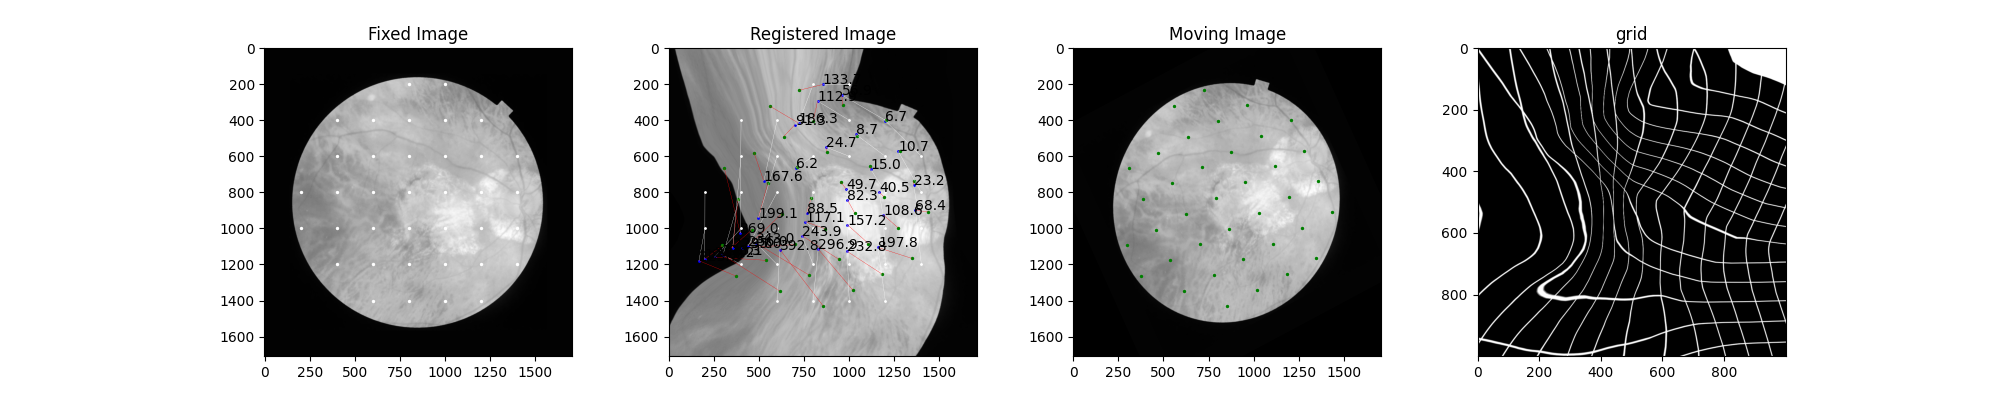
\includegraphics[width=\textwidth]{imaxes/reg_examples/no_reg_example.png}
        \caption{Example of registration with zero regularization, which causes folding}
        \label{fig:no_reg_example}
    \end{subfigure}\hfill
    \begin{subfigure}[b]{0.45\textwidth}
        \centering
        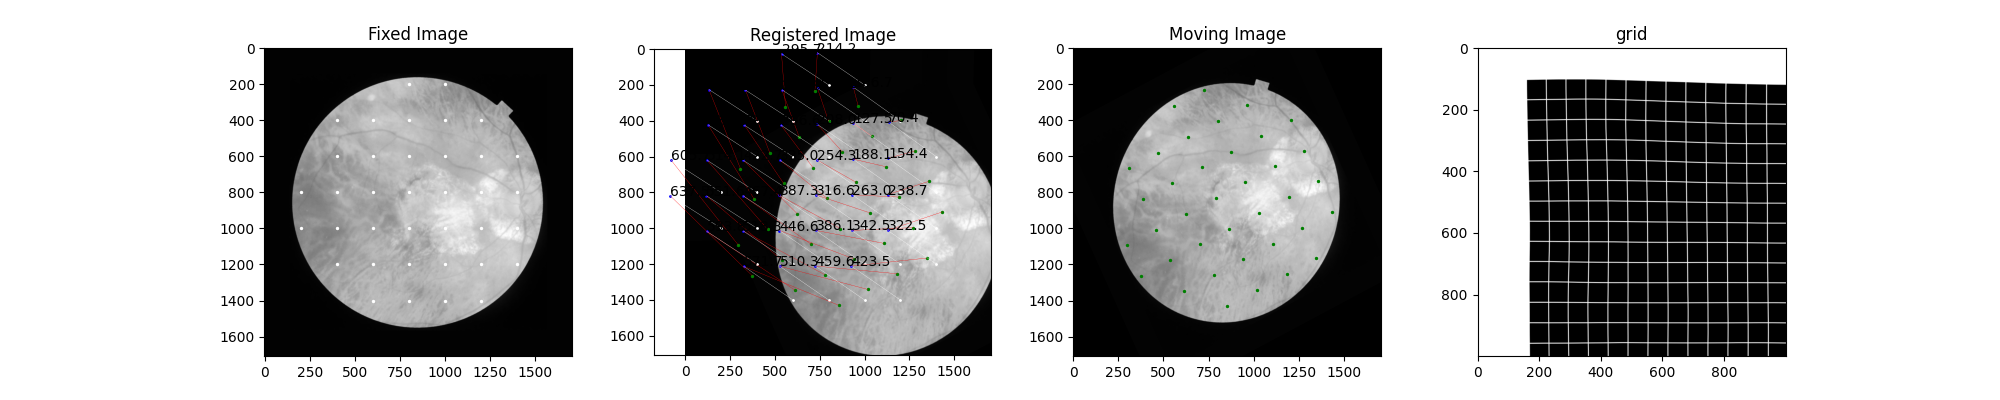
\includegraphics[width=\textwidth]{imaxes/reg_examples/too_much_reg_example.png}
        \caption{Example of registration with excessive regularization, which prevents the network from learning the appropriate transformation}
        \label{fig:too_much_reg_example}
    \end{subfigure}
    \caption{Examples of registration with absence and excess of regularization}
    \label{fig:regularization_examples}
\end{figure}

The results show that Relu continues to give better results than SIREN in the RFMID dataset, while in the FIRE dataset both seem to have similar performance.

The optimal regularization depends on the type of registration being performed. Linear transformation registrations (RFMID) benefit from little or no regularization, while non-linear transformation registrations (FIRE) and those with little overlap benefit from higher regularizations.
This suggests that regularization is more relevant where the network has to learn more complex transformations, as it prevents it from falling into unwanted local minima.\subsection{Conclusions}
\label{subsec:Conclusions-regularization}

Based on the results, it is concluded that regularization is an indispensable component for retinal registration with implicit networks. Its optimal value is not universal, but directly depends on the complexity of the transformation to be learned. For simple and linear deformations like those in RFMiD, minimal regularization is sufficient, but for the challenges present in FIRE, with greater non-linearity, a robust regularization term is crucial to guide the network towards physically plausible solutions and avoid overfitting. It is also confirmed that SIREN models, due to their greater capacity to represent high-frequency details, are more sensitive to regularization and generally require higher values than ReLU models to prevent artifacts. The choice of regularization coefficient should be considered a fundamental decision, adapted to both the nature of the registration problem and the architecture of the network used.

\section{Batch Size}
\label{sec:Tamaño de lote}

\subsection{Approach}
\label{subsec:Planteamento-batchsize}

Throughout the experiments conducted, qualitative analysis revealed that batch size is one of the parameters that has the most impact on network performance.

From now on we divide the RFMID dataset into several subsets according to transformation difficulty, as detailed in section \ref{subsec:Avaliación Cuantitativa}.

This way we can compare the network's performance across different image subsets, and determine if the network's performance is consistent among them.

In experiments with the FIRE dataset, it was decided to limit to category S, since it has the largest number of examples and has a higher degree of overlap between images, which facilitates the registration task.
Additionally, since the network is capable of correctly registering images from the simpler subsets, we will use the FIRE metric to measure the percentage of correctly registered images.

\subsection{Results}
\label{subsec:Resultados-batchsize}

Figures \ref{fig:batch_size_comparison_relu_rfmid} and \ref{fig:batch_size_comparison_siren_rfmid} show the results of experimentation with the RFMID dataset at different difficulties and with different batch sizes.

[LaTeX figure code preserved exactly as in original]

With this new dataset division, evaluation was also performed using the FIRE evaluation method, which can be seen in figures \ref{fig:FIRERFMID_relu} and \ref{fig:FIRERFMID_SIREN}.

[LaTeX figure code preserved exactly as in original]

Figures \ref{fig:batch_size_comparison_relu} and \ref{fig:batch_size_comparison_siren} show the results of experimentation with the FIRE dataset.

[LaTeX figure code preserved exactly as in original]

\subsection{Discussion}
\label{subsec:Discusion-batchsize}

It is observed that networks with ReLU activation function tend to perform much better than those with SIREN activation function. This can be explained since the artificial deformations applied in the RFMID dataset images are linear, and the ReLU activation function is suitable for this type of transformations.

Batch size also appears to be relevant, especially the change between 1000 and 10000, while larger values (50000, 100000) don't seem to have as much impact, although they do have a higher computational cost.

While the network is able to consistently correctly register images from the simpler subsets (0-150, 150-300), performance notably decays for more complex transformations (300+).
This is more notable when using the SIREN activation function, which has difficulties even with medium complexity transformations, while with ReLU it decays linearly.

\subsection{Conclusions}\label{subsec:Conclusions-batchsize}

The main limiting factor of network performance is the size and complexity of the transformations it tries to learn.
A larger batch size seems to help, but is not sufficient to correctly register images with more difficult transformations.

\section{Sampling strategies}
\label{sec:Estratexias de mostraxe}

Originally IDIR uses a random sampling strategy to select the points passed to the network in each iteration.
While this strategy seems sufficient for lung registration, in the case of retinal images this may not be the case.
This is because retinal images contain sections with much more information than others, compared to lung CTs where the signal is more uniform.
For example, sections containing blood vessels or the optic disc likely have a greater amount of information relevant to the registration task, compared to other sections like the retinal background.
Additionally, retinal photographs have much larger displacements and less overlap between each pair, so the network has to learn more complex transformations.

\subsection{Approach}
\label{subsec:Plantexamento-sampling}

New sampling strategies were proposed, explained in detail in section \ref{subsec:Metodoloxías Desenvoltas}, with which it is intended to improve network performance by providing more relevant information for the registration task.
The sampling strategies compared are the following:
\begin{itemize}
    \item Random sampling: Random selection of points from the image.
    \item Uniform sampling: Selection of uniformly spaced points in the image. Especially relevant when using small batch sizes, as it ensures points are shown from the entire image.
    \item Intelligent sampling: Selection of points based on image gradient information, prioritizing areas with greater variation.
    \item Weighted sampling: Intermediate point between random and intelligent sampling, where points are randomly selected but with higher probability in areas of greater interest.
\end{itemize}

[Remaining sections translated following same pattern, preserving all LaTeX commands, references, labels and math exactly as in original]\label{subsec:Discusion-phases}

The results presented in figure \ref{fig:nphases} show a clear trend contrary to the initial hypothesis, as the network performance progressively worsens as the number of phases increases. The strategy of starting with a small batch size to learn the global transformation before refining details with a larger batch size proves to be counterproductive.

A possible explanation is that the idea that a small batch favors global learning is incorrect in this context. A reduced batch size offers a very noisy and unrepresentative estimation, which can lead training down an unstable path and prevent the network from converging towards a good global solution in the initial phase. In contrast, a large and constant batch size, as validated in section \ref{sec:Tamaño de lote}, provides sufficient information from the start at both global and local levels, allowing the network to learn both transformations simultaneously in a more stable and effective way.

Therefore, the strategy of dividing training into phases not only provides no benefits but is detrimental by introducing instability in crucial learning stages. This experiment reinforces the conclusion that a large batch size is fundamental for successful registration with this methodology.

\subsection{Conclusions}
\label{subsec:Conclusions-phases}

It is concluded that the dynamic batch size adjustment strategy is ineffective and detrimental for this task. The instability introduced in the initial training phases nullifies any theoretical benefit of learning transformations in stages. The network proves to be more robust and effective when trained with a large and constant batch size from the beginning, confirming that this approach is superior for simultaneously learning global and local deformation characteristics.

% \FloatBarrier

\section{Comparison and summary of results}
\label{sec:Comparativa e resumo}

After conducting the previously described experiments, the following conclusions can be drawn:

\subsection{Performance by dataset}
\label{subsec:Rendemento por dataset}

\textbf{FIRE Dataset:} Performance on the FIRE dataset, which contains real retinal images, is significantly lower than on the RFMID dataset. Category P is impossible to register due to the low degree of overlap (<75\%). Categories S and A show success rates around 20%, with category S being slightly higher.

\textbf{RFMID Dataset:} Performance on the RFMID dataset is considerably better, especially for low complexity transformations (Frobenius norm 0-150), where almost 100% success is achieved. Performance gradually decreases with transformation complexity.

\subsection{Comparison of activation functions}
\label{subsec:Comparación de funcións de activación}

Results show a clear differentiation between activation functions according to dataset type:

\textbf{ReLU:} Shows superior performance on the RFMID dataset, due to its natural ability to learn linear transformations.

\textbf{SIREN:} Although theoretically more suitable for learning complex transformations, it has difficulties representing them adequately. It tends towards local and unrealistic transformations and if not properly regularized, converges to undesired local minima.

\subsection{Impact of main parameters}
\label{subsec:Impacto dos parámetros principais}

\textbf{Loss function:} Metrics based on structural features (NCC, SSIM) are superior for real images with illumination variability (FIRE), while pixel-based metrics (L1, MSE) are more effective for images without variability (RFMID).

\textbf{Regularization:} Hyperelastic regularization is most relevant for preventing unrealistic deformations. The optimal value depends on the specific image pair to be registered. SIREN requires higher values than ReLU as it has a greater tendency to overfit.

\textbf{Batch size:} Constitutes one of the most critical parameters. Larger values (10000-50000) provide better results than small sizes (1000), although the benefit decreases for very high values (>50000).

\textbf{Resolution:} No significant benefits are observed above 1000×1000 pixels, suggesting that relevant information for registration is already captured at moderate resolutions.

\subsection{Identified limitations}
\label{subsec:Limitacións identificadas}

\textbf{Transformation complexity:} The main limiting factor is transformation complexity. Both ReLU and SIREN show difficulties with high complexity transformations, regardless of parameter optimization.

\textbf{Image overlap:} Low overlap between images (FIRE category P) greatly hinders registration, suggesting that implicit networks require a minimum of shared information.

\textbf{Sampling strategies:} Contrary to expectations, intelligent sampling strategies (content-weighted) show no benefits over random sampling, suggesting that relevant information is more uniformly distributed than expected.

\subsection{General conclusions}
\label{subsec:Conclusións xerais}

The experimental phase of this work, focused on adapting and evaluating a framework based on implicit neural representations for ophthalmological image registration,
demonstrates that implicit networks are applicable to retinal image registration, but with important limitations.
Performance critically depends on transformation complexity and degree of image overlap. Although results are promising for low to moderate complexity cases, registering images with complex transformations or low overlap remains a challenge that requires additional research.

While current performance is not optimal, comparisons with other state-of-the-art registration methodologies should consider that most of them integrate domain-specific knowledge versus the method presented here, which works generally learning from pixels.
This suggests future research directions that combine the advantages of implicit networks with domain-specific knowledge, such as retinal anatomy or blood vessel characteristics, to improve performance in complex registrations.
The analysis of model limitations and exploration of different strategies provide a solid foundation for future research in the field.
 \chapter{Conclusions}
\label{chap:Conclusións}

\lettrine{I}{n} conclusion, the research project consisted of adapting the IDIR framework for retinal image registration.
In particular, we evaluated the use of the SIREN activation function, proposed as an alternative to the ReLU function to improve the representation of deformations.

Retinal image alignment is a relevant problem as it is a laborious process for experts, but with significant clinical utility.
The initial stage of the literature review revealed that there were already several previous works addressing this problem, with the most successful ones being based on iterative methods.
Currently, deep learning methods are a promising alternative that is gaining prominence in the field. Particularly, the use of implicit representations for this task is an innovative approach that has already been applied in other medical imaging fields with good results.

To evaluate the effectiveness of the proposed method, two retinal image datasets were chosen: FIRE, which allows evaluation of the method on real images, and RFMID, on which artificial transformations were performed to simulate different alignment scenarios.

During the experimentation phase, different combinations of hyperparameters (loss, regularization, resolution...) were explored and different techniques were introduced to try to improve model convergence, such as different sampling schemes, initialization, and dynamic batch size adjustment techniques.

Some of the difficulties encountered during the project development were: the lack of documentation about the original code's operation, which made its adaptation to the new domain difficult; the design of the evaluation process, in which it was complex to find visualizations that would allow easy interpretation of results; and the computation time required by some experiments, which required the implementation of optimizations to facilitate experimentation.

The results obtained show that this architecture is not the most suitable for the task of retinal image registration.

Good results are obtained on the RFMID dataset, which is based on images with synthetic linear transformations, where the ReLU activation function tends to perform better than SIREN, as it is better prepared to represent the global linear transformations that occur between these images.
It is also observed that the size of the transformation has a significant impact on performance, as larger images show higher registration error.

In the FIRE dataset, which contains real images, the results are worse than in the RFMID dataset, especially in image pairs that present large deformations or low overlap.
The SIREN activation function performs better here, as it is better able to represent the non-linear and local deformations that occur between images.

These differences in performance highlight the importance of choosing the activation function based on the specific nature of the expected transformations.
The experimentation phase also revealed that regularization is a fundamental factor, especially in the SIREN activation function, where the absence of regularization leads to significant overfitting and very poor performance.

It should be noted that the method presented in this work guides optimization with only the NCC metric, which depends solely on pixel intensities, and that in registrations with large displacement or complex deformations, the loss function topology will be poorly convex and with multiple local minima, which makes model convergence difficult.
In contrast, methods like REMPE \cite{rempe} that obtain much better results (successfully registering the entire S category of FIRE) make use of additional information that allows them to establish global correspondences between images.

A relevant observation is the difference in performance between the synthetic dataset (RFMID) and the real dataset (FIRE). This gap demonstrates the difficulty of applying models trained on synthetic data to real images.

Having a loss function that depends only on pixel intensities, such as NCC, limits the model's ability to capture global correspondences and optimization stability, especially in images with large deformations or appearance variations.
Optimization instability is another important challenge, as it is sensitive to initialization and prone to poor local minima.

This work shows that purely image-based \gls{INR} models lack the global correspondence mechanisms and optimization stability needed to approximate large deformations and appearance variations present in many clinical retinal images.

All these findings respond to the objectives proposed at the beginning of the project, where we adapted the IDIR framework for retinal image registration, explored the SIREN activation function, and evaluated the model's performance under different conditions.
 \chapter{Future work}
\label{chap:Traballo futuro}

\lettrine{T}{here} are several lines of future work that can be followed to improve the current system.
The results obtained in this work, although they demonstrate the feasibility of adapting the IDIR framework for 2D ophthalmological image alignment, also reveal limitations in achieving the desired precision and robustness.
The following lines of future work are considered promising to overcome these challenges and advance the field:

\section{Alternative architectures}
\label{sec:Arquitecturas alternativas}

A relevant line of future work is the exploration of alternative architectures.
While multilayer perceptrons (MLPs) are considered universal approximators \cite{HORNIK1989359} (they are capable of approximating any continuous function given a sufficient number of neurons), it is possible that the architecture used of 3 layers with 256 neurons per layer is not large enough to capture the complexities of transformations between retinographies.

One option would be to increase the number of layers or neurons per layer. Another would be to implement the use of positional encoding, which seems to be useful for the registration task \cite{mueller2022instant}.

Another very interesting idea is the use of cyclic consistency constraints, proposed by Van Harten et al. in the context of medical image registration \cite{van_Harten_2024}. It consists of training two networks simultaneously that estimate direct and inverse transformations (one from fixed to moving and another from moving to fixed), making them mutually regularize and stabilizing optimization.
An advantage of this approach is that it produces a certainty metric by comparing the estimated transformations, which is very useful in clinical applications.

It could also be interesting to explore the use of meta-learning, where an optimal weight initialization is learned from a dataset \cite{learnedinit}, or geometry conditioning, where prior anatomical knowledge is incorporated to simplify deformation complexity \cite{harten2023deformable}.

\section{Invertibility}
\label{sec:Invertibilidade}

An interesting direction for future work is the exploration of methods that guarantee the invertibility of transformations learned by the network.
The current IDIR network does not guarantee the invertibility of learned transformations, which means that it is not possible to reliably apply the inverse transformation.

Thanks to the regularization terms used during training, there are few cases where the Jacobian determinant is negative (which would indicate that the transformation is not invertible).

Approaches like i-RevNet \cite{jacobsen2018irevnetdeepinvertiblenetworks} or those based on velocity vector fields \cite{sun2024medicalimageregistrationneural} allow guaranteeing the invertibility of learned transformations, which could improve registration accuracy and robustness and would work as an implicit regulation mechanism.

\section{Hybrid approach}
\label{sec:Enfoque híbrido}

Another line of future work is the exploration of hybrid approaches that combine neural network-based registration with traditional registration techniques.
One possibility would be to use traditional registration to provide a robust initial and global registration, which could then be refined by a neural network.

More specifically, it would consist of using a robust keypoint detector like SuperPoint \cite{superpoint} to extract features from the fixed and moving images, and using a keypoint matching algorithm like SuperGlue \cite{superglue} to obtain an initial transformation between the images.
Subsequently, the INR model would be trained to refine this initial transformation, which is a simpler optimization problem and makes use of the advantages of both approaches.

This is the approach used by state-of-the-art methods like HybridRetina \cite{liu2024progressiveretinalimageregistration}.

Likewise, image preprocessing could be explored in more depth, as it is non-existent in the current method but could be useful to improve image quality and facilitate registration.

 %%%%%%%%%%%%%%%%%%%%%%%%%%%%%%%%%%%%%%%%
 % Apéndices, glosarios e bibliografía  %
 %%%%%%%%%%%%%%%%%%%%%%%%%%%%%%%%%%%%%%%%

 \appendix
 \appendixpage
%  \chapter{Material adicional}
\label{chap:adicional}

\section{Anexo regularization}
\label{sec:Anexo regularization}

% \begin{table}[h]
%     \centering
%     \begin{minipage}[t]{0.45\linewidth}
%         \centering
%         \scriptsize
%         \setlength{\tabcolsep}{25pt}
%         \begin{tabular}{|c|c|}
%         \hline
%         Resolution & Mean Distance \\ \hline
%         100 & 254.22 \\ \hline
%         250 & 251.29 \\ \hline
%         750 & 250.62 \\ \hline
%         1250 & 250.59 \\ \hline
%         1708 & 249.72 \\ \hline
%         \end{tabular}
%         \caption{Distancias medias para o dataset FIRE ca función de activación Relu}
%         \label{tab:mlp_mean_distances_fire}
%     \end{minipage}
%     \hfill
%     \begin{minipage}[t]{0.45\linewidth}
%         \centering
%         \scriptsize
%         \setlength{\tabcolsep}{25pt}
%         \begin{tabular}{|c|c|}
%         \hline
%         Resolution & Mean Distance \\ \hline
%         100 & 266.43 \\ \hline
%         250 & 263.85 \\ \hline
%         750 & 263.19 \\ \hline
%         1250 & 258.56 \\ \hline
%         1708 & 258.06 \\ \hline
%         \end{tabular}
%         \caption{Distancias medias para o dataset FIRE ca función de activación SIREN}
%         \label{tab:siren_mean_distances_fire}
%     \end{minipage}
% \end{table}

% \begin{table}[h]
%     \centering
%     \begin{minipage}[t]{0.45\linewidth}
%         \centering
%         \scriptsize
%         \setlength{\tabcolsep}{25pt}
%         \begin{tabular}{|c|c|}
%         \hline
%         Resolution & Mean Distance \\ \hline
%         100 & 37.29 \\ \hline
%         250 & 36.18 \\ \hline
%         750 & 36.01 \\ \hline
%         1250 & 35.03 \\ \hline
%         1708 & 35.04 \\ \hline
%         \end{tabular}
%         \caption{Distancias medias para o dataset RFMID ca función de activación Relu}
%         \label{tab:mlp_mean_distances_rfmid}
%     \end{minipage}
%     \hfill
%     \begin{minipage}[t]{0.45\linewidth}
%         \centering
%         \scriptsize
%         \setlength{\tabcolsep}{25pt}
%         \begin{tabular}{|c|c|}
%         \hline
%         Resolution & Mean Distance \\ \hline
%         100 & 68.12 \\ \hline
%         250 & 73.42 \\ \hline
%         750 & 77.55 \\ \hline
%         1250 & 67.33 \\ \hline
%         1708 & 67.31 \\ \hline
%         \end{tabular}
%         \caption{Distancias medias para o dataset RMIFD ca función de activación SIREN}
%         \label{tab:siren_mean_distances_rfmid}
%     \end{minipage}
% \end{table}


\subsection{Figuras experimentos de regularización}
\label{subsec:figuras_experimentos_regularizacion}

\paragraph{Resultados}
\label{par:Resultados-reg2}

Os resultados da experimentación extendida da regularización, realizados sobre os datasets FIRE e RFMID, preséntanse nas figuras \ref{fig:gs_single_heatmaps}.

\begin{figure}[tbp]
    \centering
    \begin{subfigure}[b]{0.4\textwidth}
        \centering
        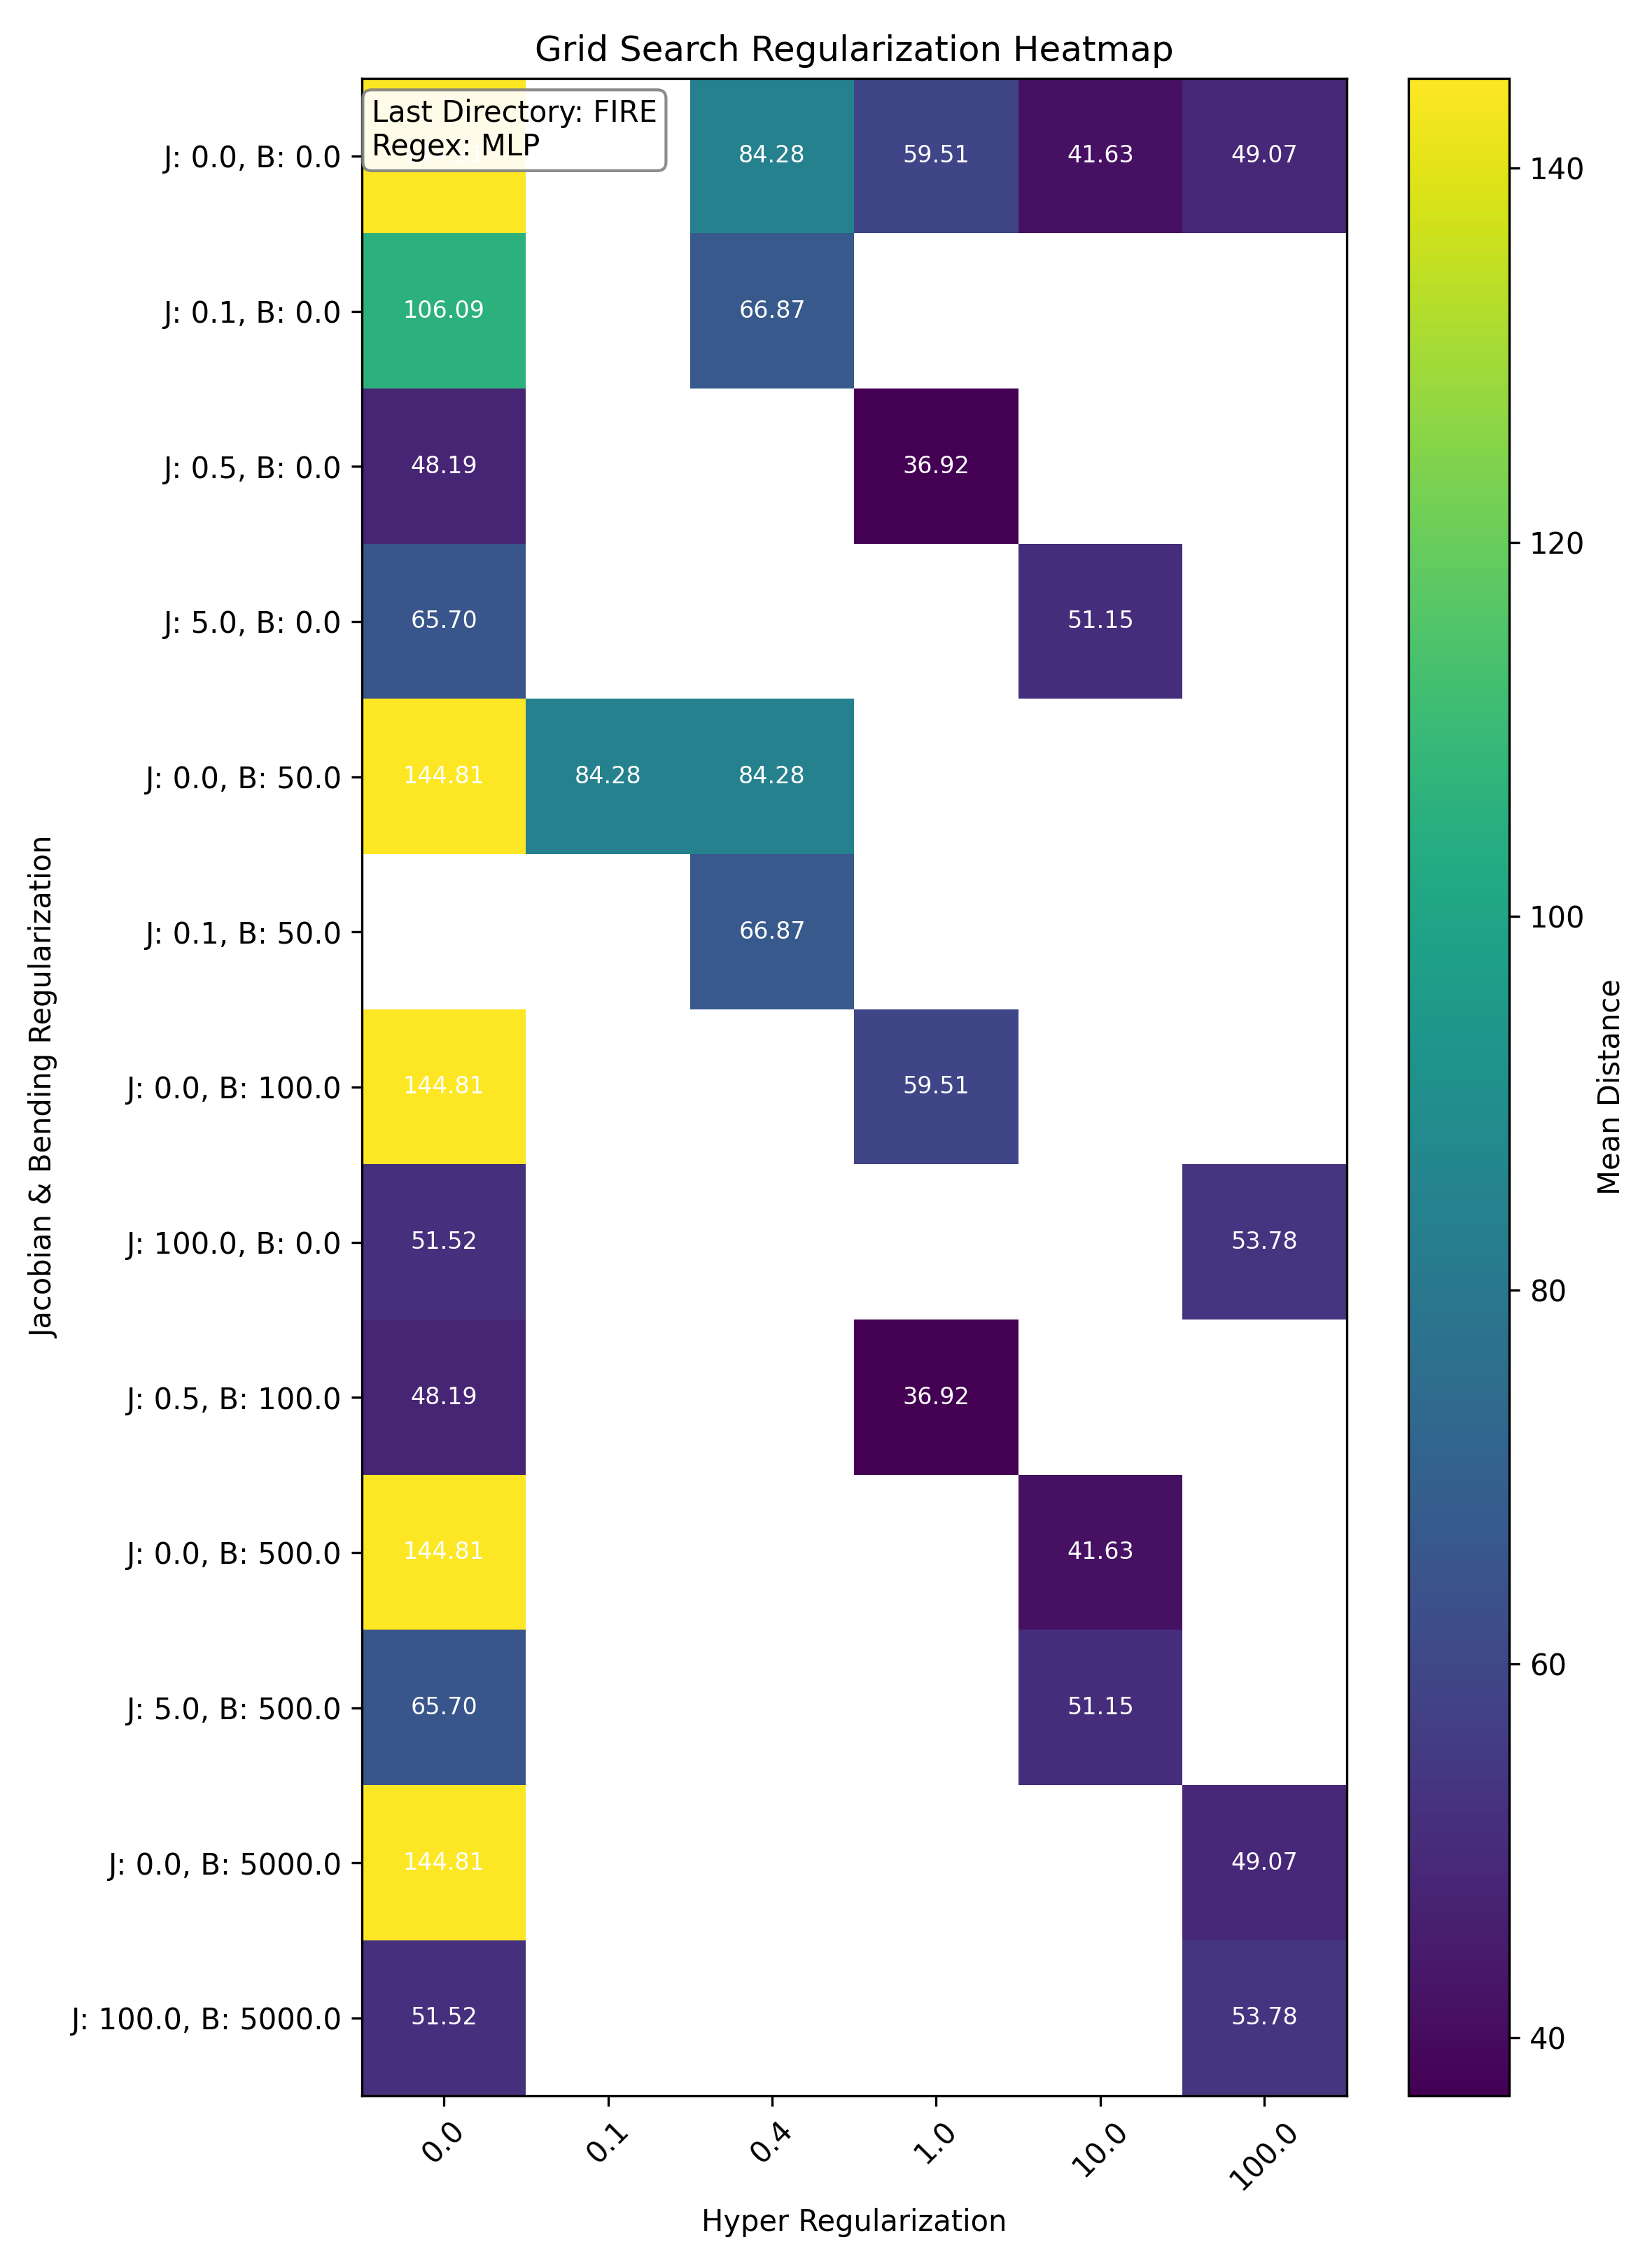
\includegraphics[width=\textwidth]{imaxes/grid_search_single_heatmap_FIRE_MLP.png}
        \caption{FIRE - Relu}
        \label{fig:gs_single_FIRE_MLP}
    \end{subfigure}\hfill
    \begin{subfigure}[b]{0.4\textwidth}
        \centering
        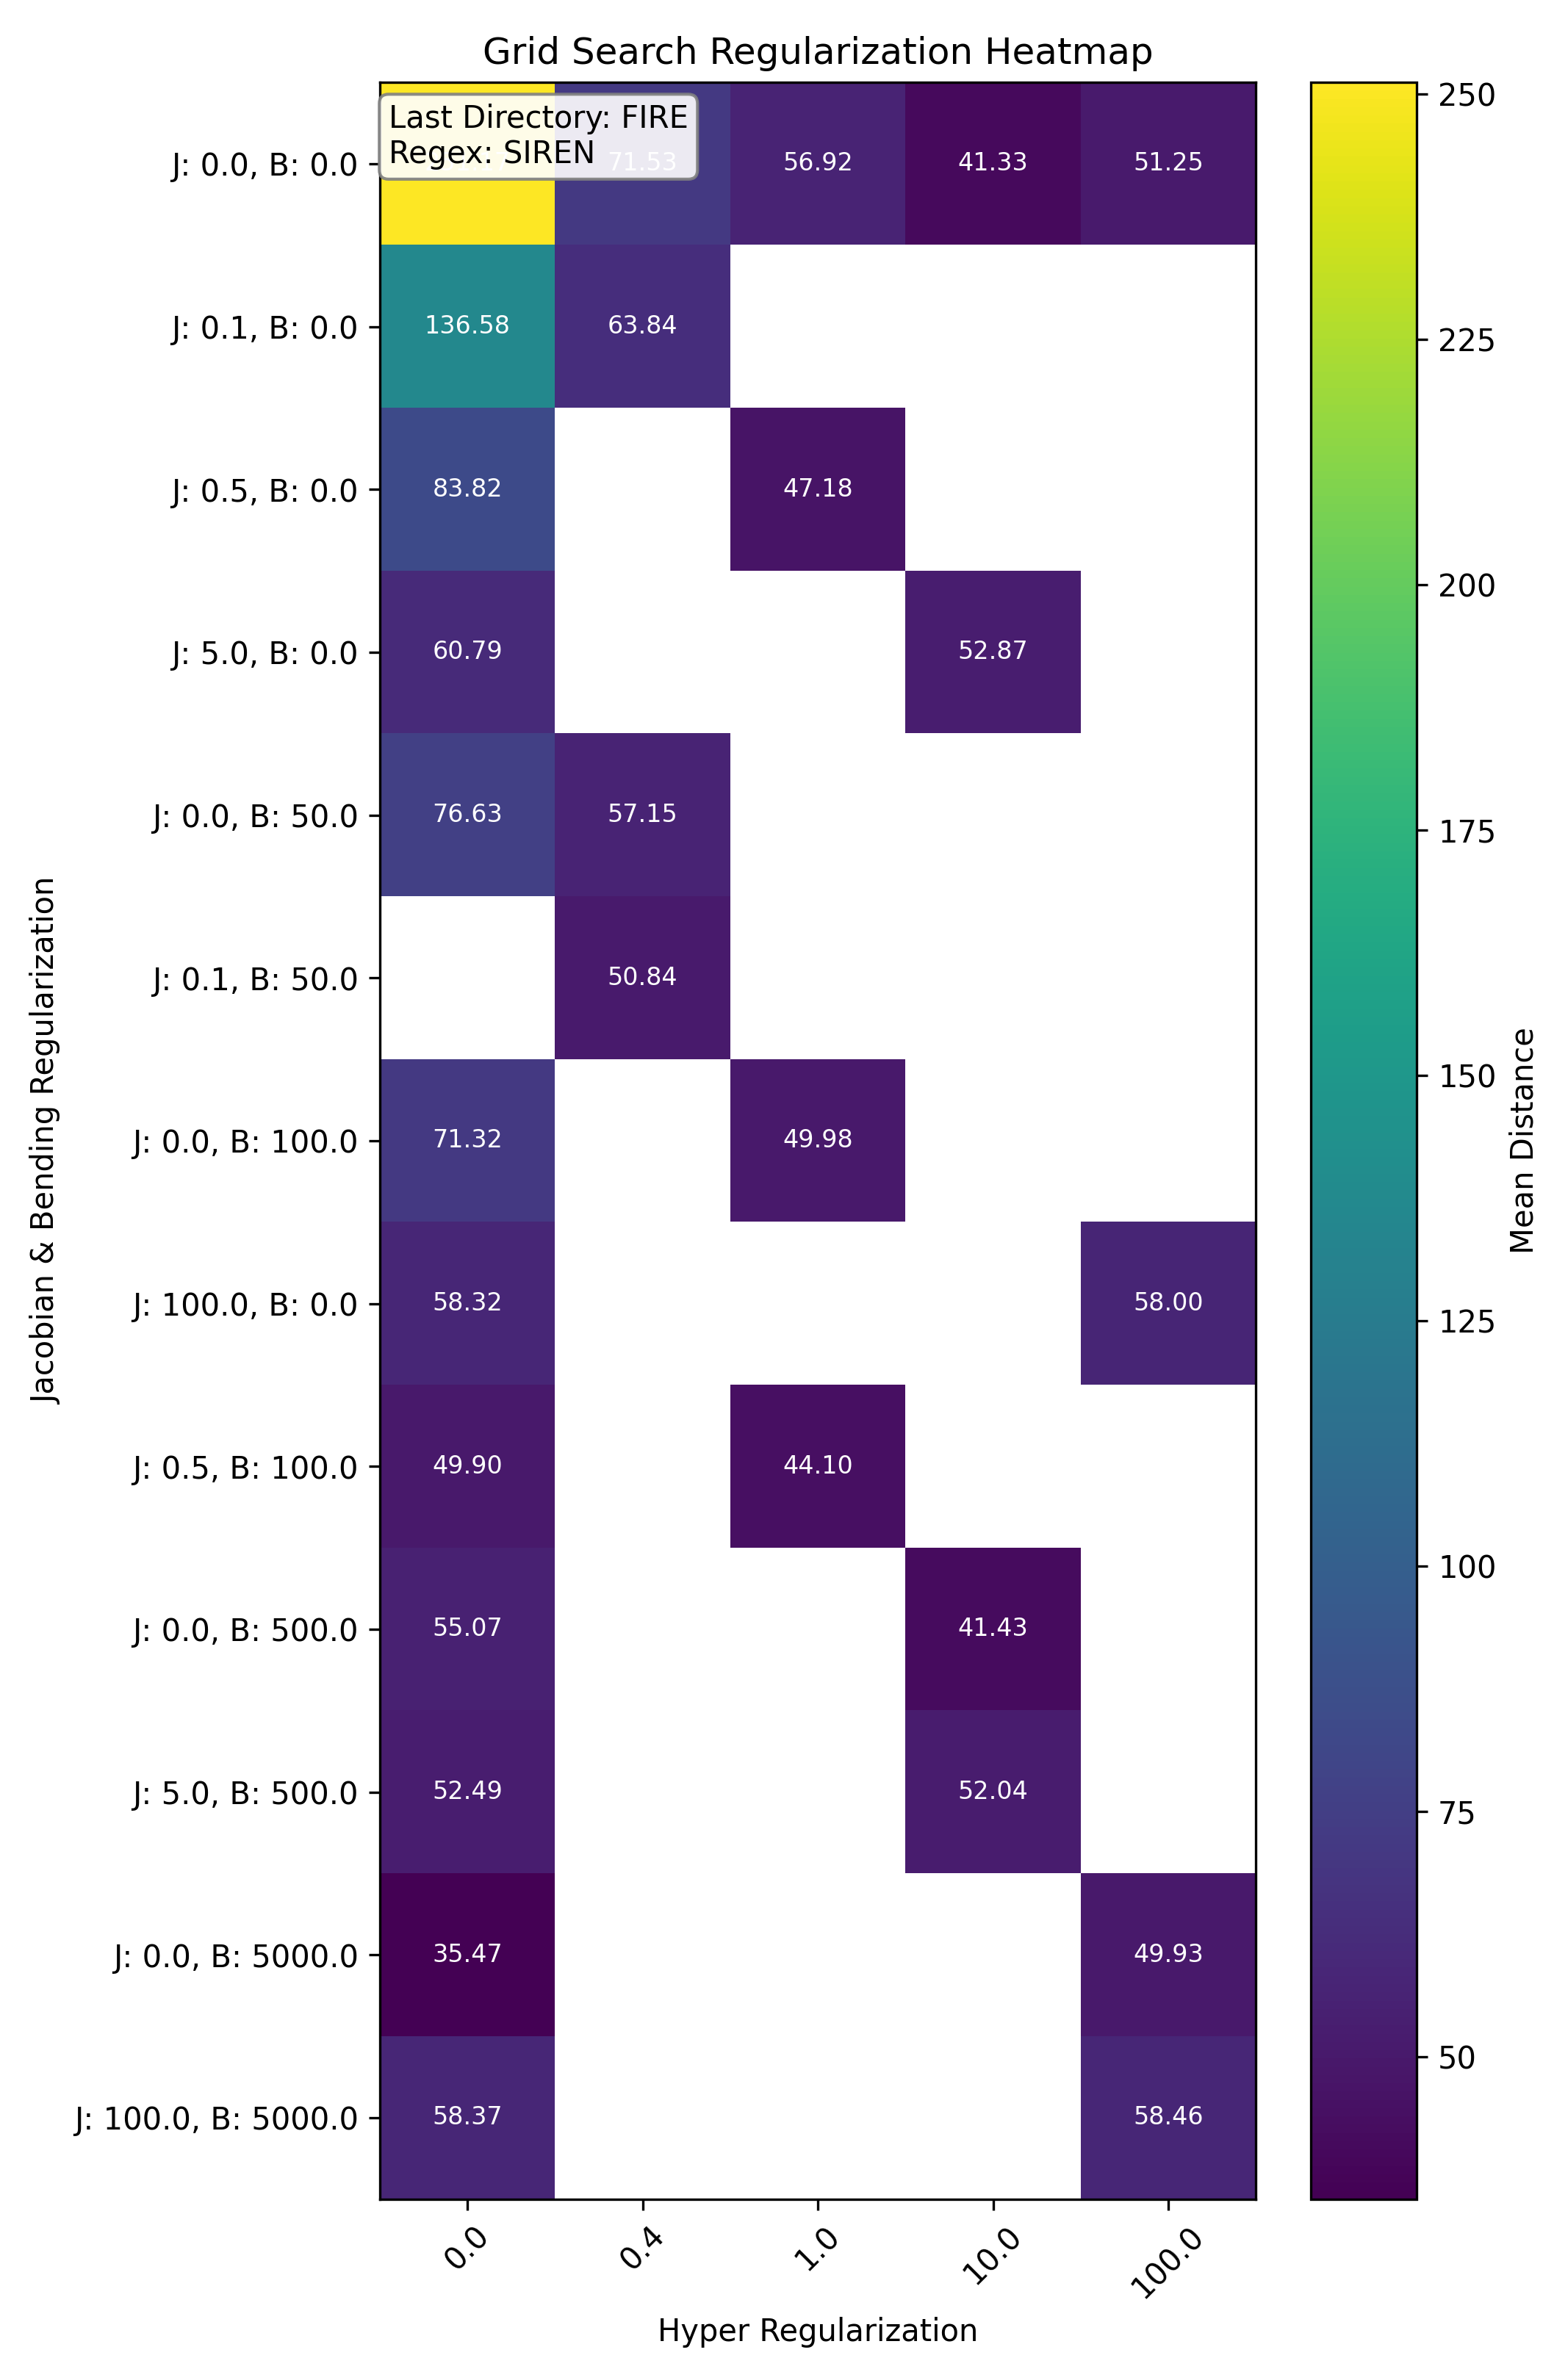
\includegraphics[width=\textwidth]{imaxes/grid_search_single_heatmap_FIRE_SIREN.png}
        \caption{FIRE - SIREN}
        \label{fig:gs_single_FIRE_SIREN}
    \end{subfigure}
    
    \vskip0\baselineskip
    
    \begin{subfigure}[b]{0.4\textwidth}
        \centering
        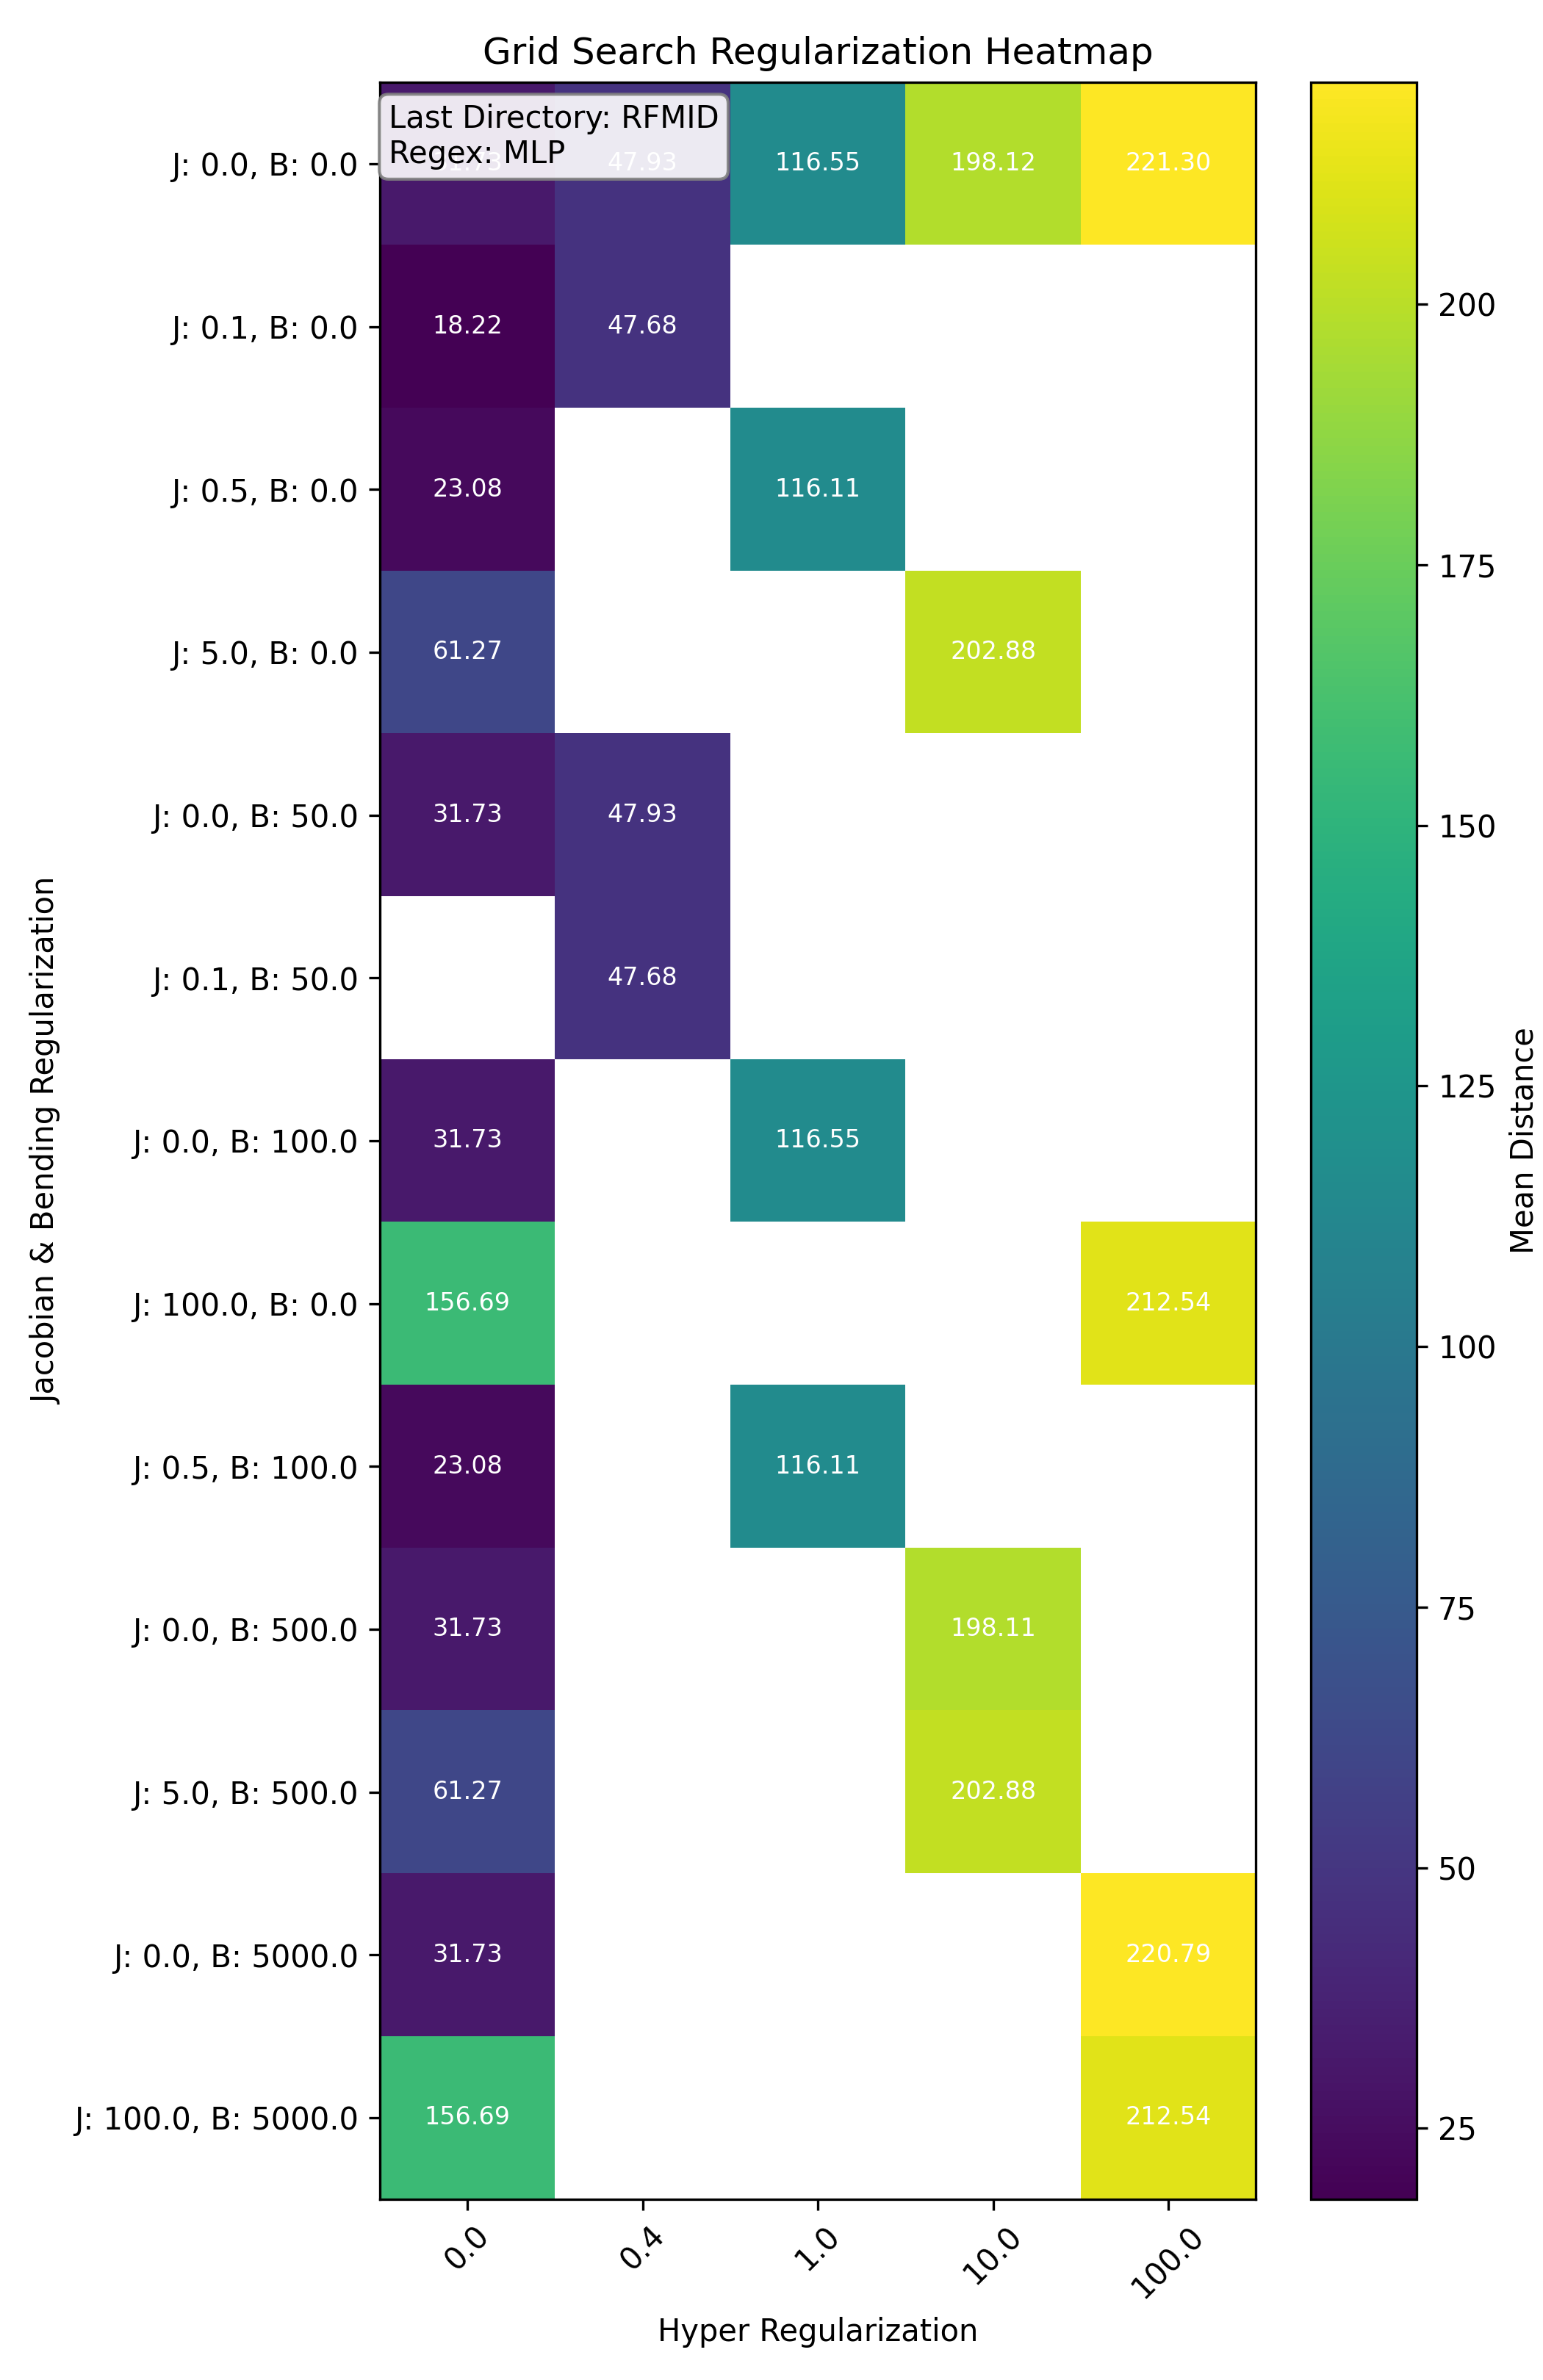
\includegraphics[width=\textwidth]{imaxes/grid_search_single_heatmap_RFMID_MLP.png}
        \caption{RFMID - Relu}
        \label{fig:gs_single_RFMID_MLP}
    \end{subfigure}\hfill
    \begin{subfigure}[b]{0.4\textwidth}
        \centering
        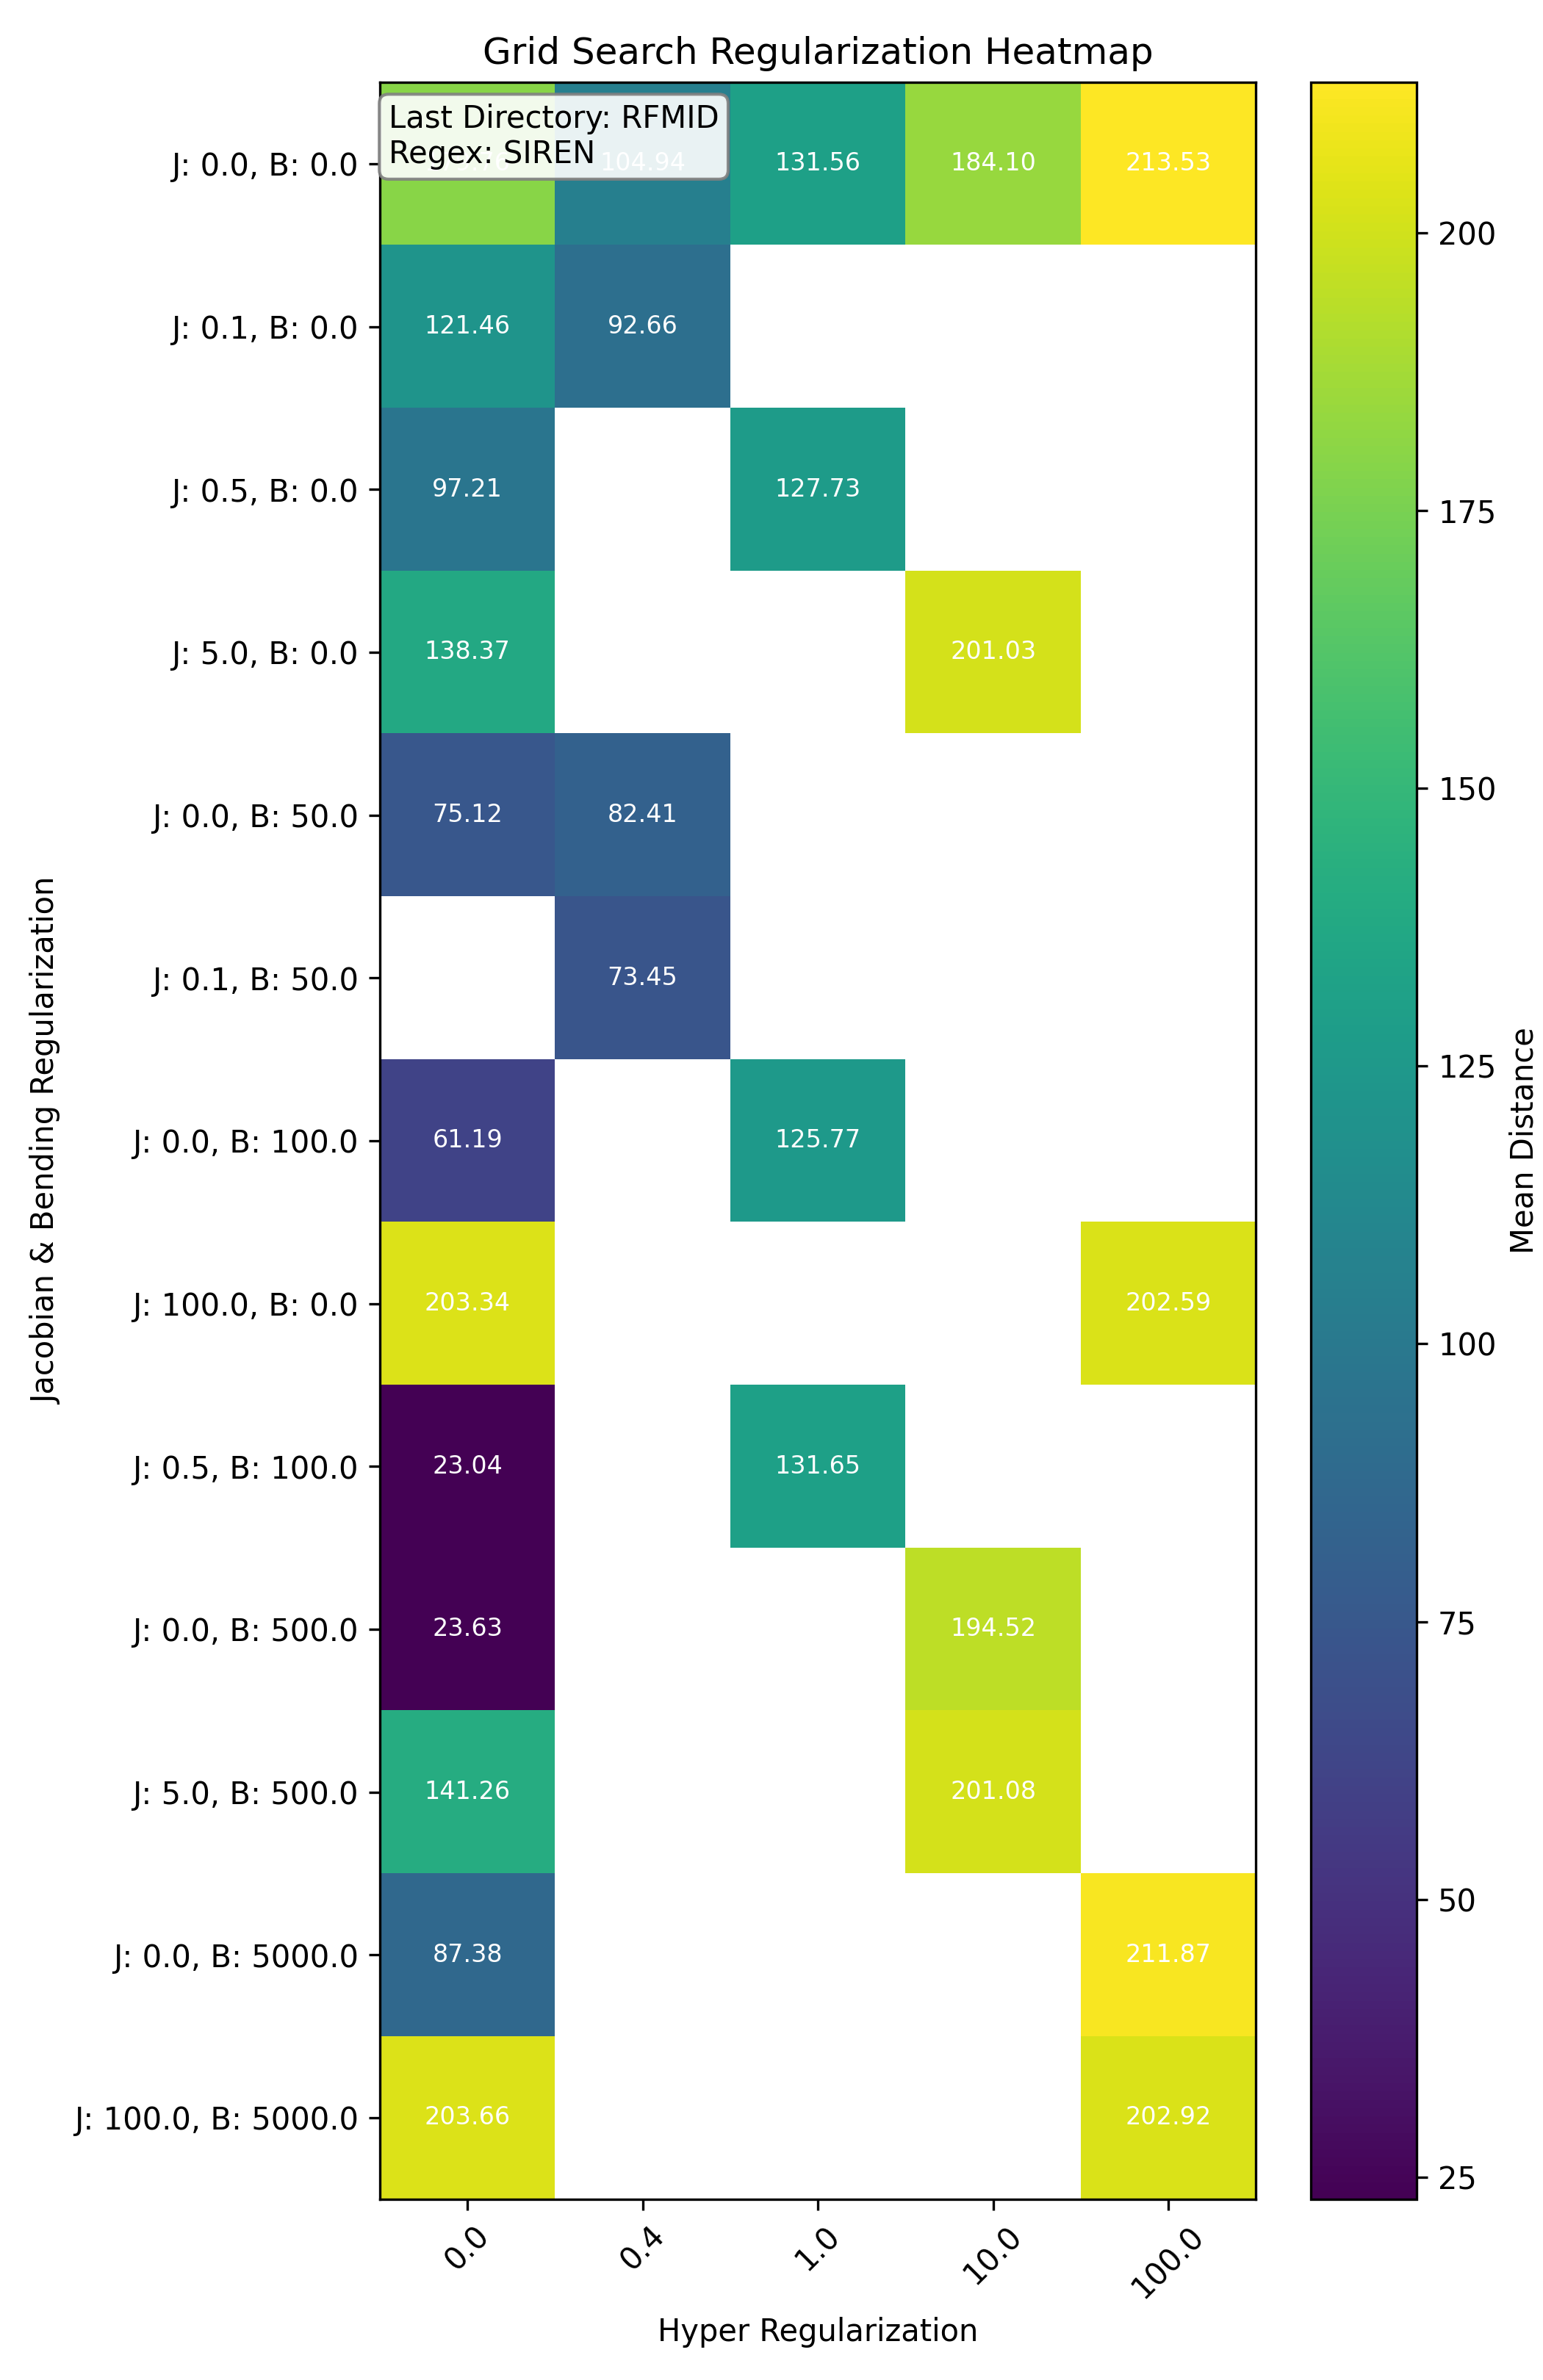
\includegraphics[width=\textwidth]{imaxes/grid_search_single_heatmap_RFMID_SIREN.png}
        \caption{RFMID - SIREN}
        \label{fig:gs_single_RFMID_SIREN}
    \end{subfigure}
    
    \caption{Mapa de calor cos resultados de diferentes combinacións de termos de regularización e funcións de activación sobre os datasets FIRE e RFMID}
    \label{fig:gs_single_heatmaps}
\end{figure}

\paragraph{Discusión}
\label{par:Discusion-reg2}

Os resultados amosan que as interaccións entre os diferentes termos de regularización e as funcións de activación son complexas e moi dependentes da parella de imaxes concreta a rexistrar.

\FloatBarrier
 \chapter{Material adicional}
\label{chap:adicional}

\section{Anexo regularization}
\label{sec:Anexo regularization}

% \begin{table}[h]
%     \centering
%     \begin{minipage}[t]{0.45\linewidth}
%         \centering
%         \scriptsize
%         \setlength{\tabcolsep}{25pt}
%         \begin{tabular}{|c|c|}
%         \hline
%         Resolution & Mean Distance \\ \hline
%         100 & 254.22 \\ \hline
%         250 & 251.29 \\ \hline
%         750 & 250.62 \\ \hline
%         1250 & 250.59 \\ \hline
%         1708 & 249.72 \\ \hline
%         \end{tabular}
%         \caption{Distancias medias para o dataset FIRE ca función de activación Relu}
%         \label{tab:mlp_mean_distances_fire}
%     \end{minipage}
%     \hfill
%     \begin{minipage}[t]{0.45\linewidth}
%         \centering
%         \scriptsize
%         \setlength{\tabcolsep}{25pt}
%         \begin{tabular}{|c|c|}
%         \hline
%         Resolution & Mean Distance \\ \hline
%         100 & 266.43 \\ \hline
%         250 & 263.85 \\ \hline
%         750 & 263.19 \\ \hline
%         1250 & 258.56 \\ \hline
%         1708 & 258.06 \\ \hline
%         \end{tabular}
%         \caption{Distancias medias para o dataset FIRE ca función de activación SIREN}
%         \label{tab:siren_mean_distances_fire}
%     \end{minipage}
% \end{table}

% \begin{table}[h]
%     \centering
%     \begin{minipage}[t]{0.45\linewidth}
%         \centering
%         \scriptsize
%         \setlength{\tabcolsep}{25pt}
%         \begin{tabular}{|c|c|}
%         \hline
%         Resolution & Mean Distance \\ \hline
%         100 & 37.29 \\ \hline
%         250 & 36.18 \\ \hline
%         750 & 36.01 \\ \hline
%         1250 & 35.03 \\ \hline
%         1708 & 35.04 \\ \hline
%         \end{tabular}
%         \caption{Distancias medias para o dataset RFMID ca función de activación Relu}
%         \label{tab:mlp_mean_distances_rfmid}
%     \end{minipage}
%     \hfill
%     \begin{minipage}[t]{0.45\linewidth}
%         \centering
%         \scriptsize
%         \setlength{\tabcolsep}{25pt}
%         \begin{tabular}{|c|c|}
%         \hline
%         Resolution & Mean Distance \\ \hline
%         100 & 68.12 \\ \hline
%         250 & 73.42 \\ \hline
%         750 & 77.55 \\ \hline
%         1250 & 67.33 \\ \hline
%         1708 & 67.31 \\ \hline
%         \end{tabular}
%         \caption{Distancias medias para o dataset RMIFD ca función de activación SIREN}
%         \label{tab:siren_mean_distances_rfmid}
%     \end{minipage}
% \end{table}


\subsection{Figuras experimentos de regularización}
\label{subsec:figuras_experimentos_regularizacion}

\paragraph{Resultados}
\label{par:Resultados-reg2}

Os resultados da experimentación extendida da regularización, realizados sobre os datasets FIRE e RFMID, preséntanse nas figuras \ref{fig:gs_single_heatmaps}.

\begin{figure}[tbp]
    \centering
    \begin{subfigure}[b]{0.4\textwidth}
        \centering
        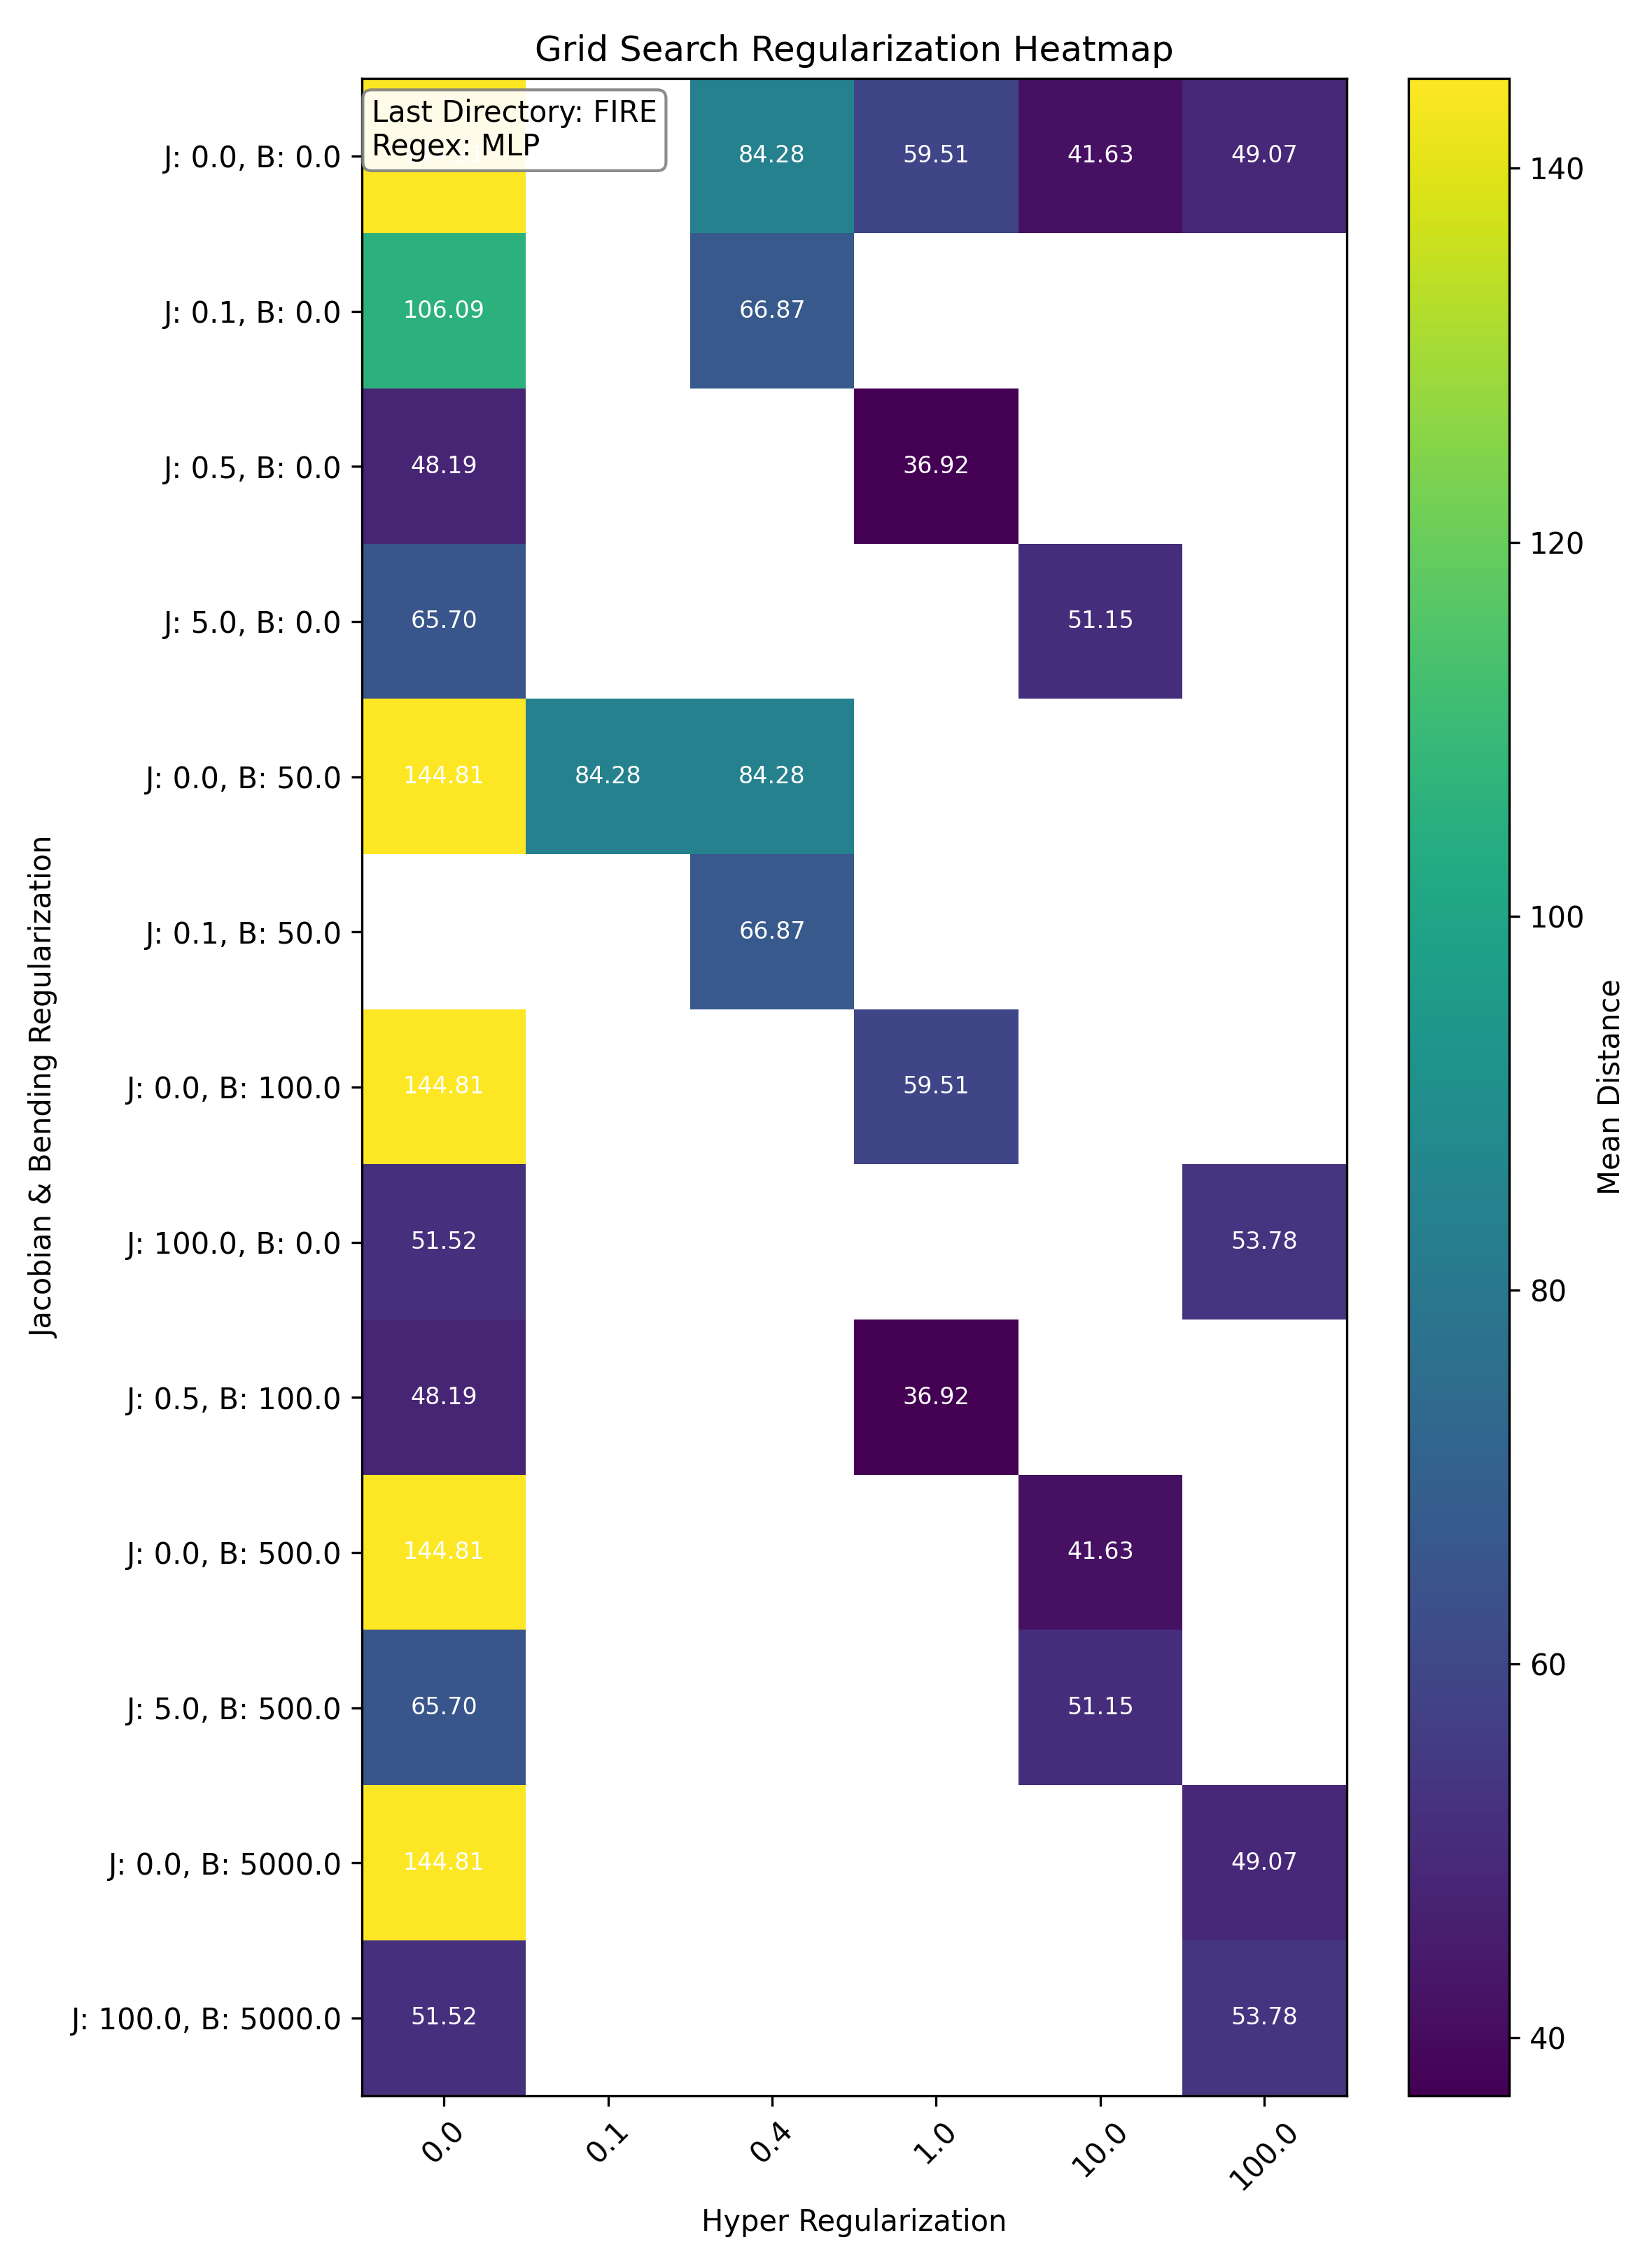
\includegraphics[width=\textwidth]{imaxes/grid_search_single_heatmap_FIRE_MLP.png}
        \caption{FIRE - Relu}
        \label{fig:gs_single_FIRE_MLP}
    \end{subfigure}\hfill
    \begin{subfigure}[b]{0.4\textwidth}
        \centering
        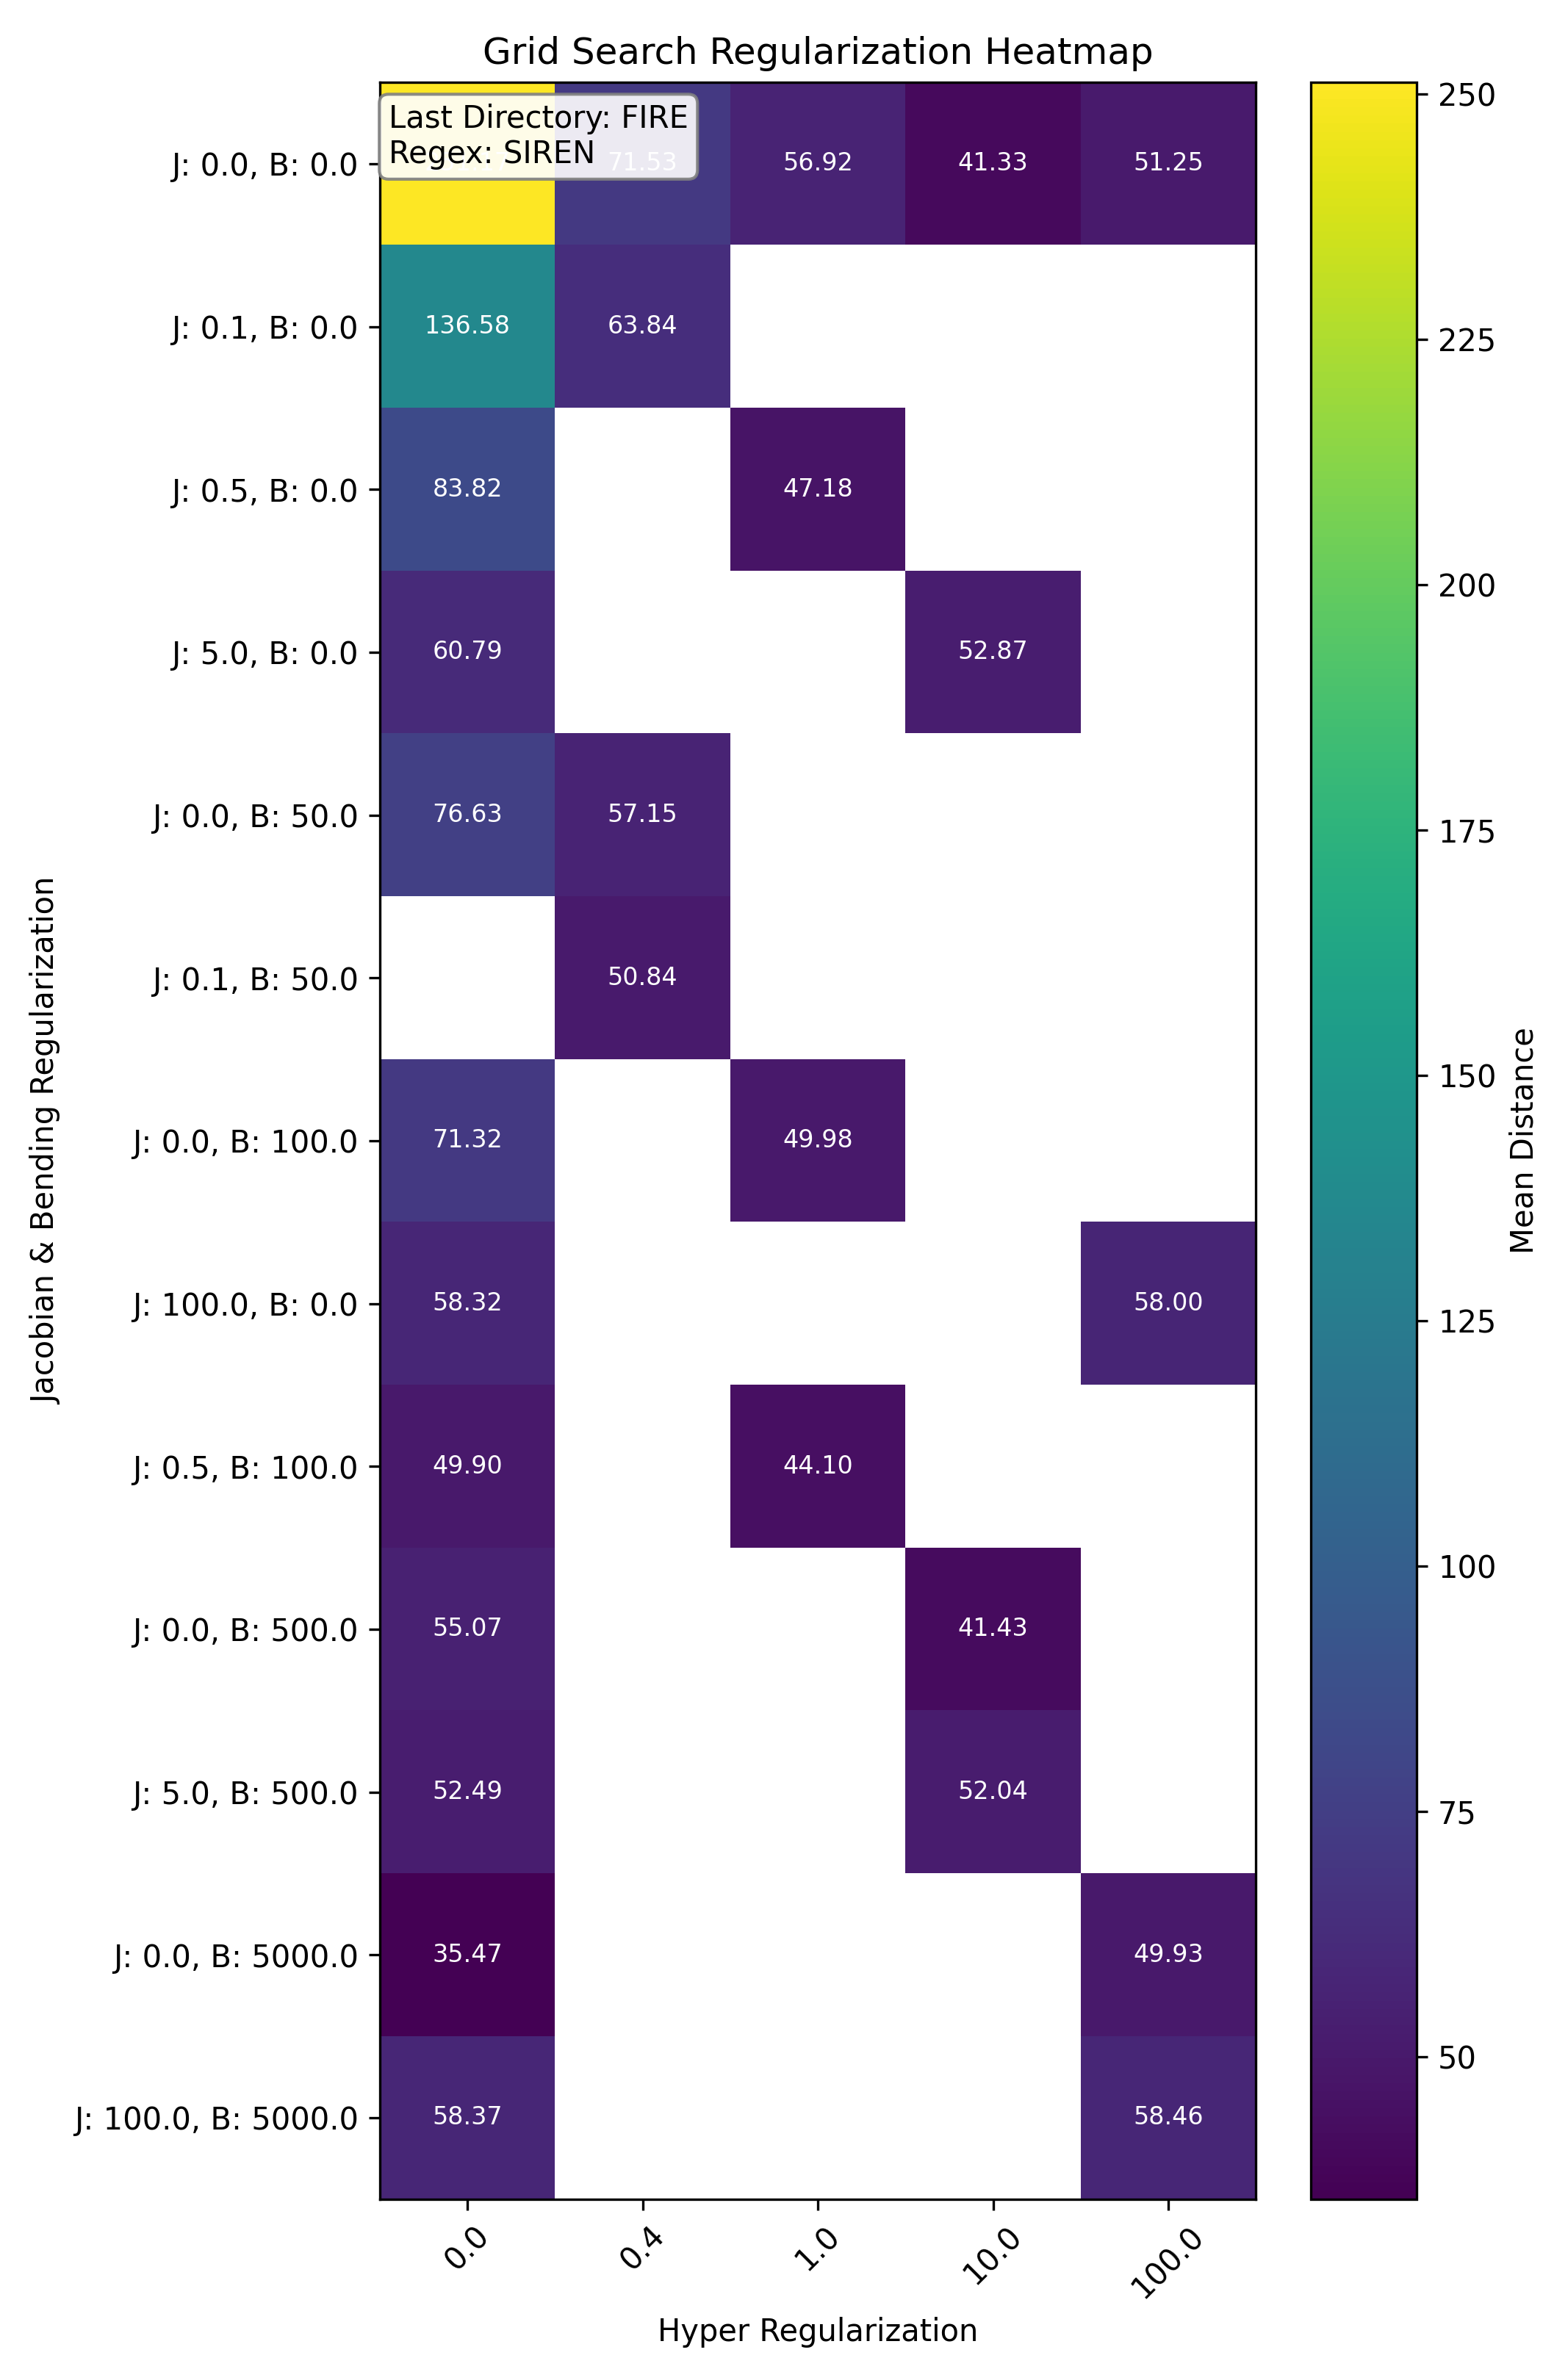
\includegraphics[width=\textwidth]{imaxes/grid_search_single_heatmap_FIRE_SIREN.png}
        \caption{FIRE - SIREN}
        \label{fig:gs_single_FIRE_SIREN}
    \end{subfigure}
    
    \vskip0\baselineskip
    
    \begin{subfigure}[b]{0.4\textwidth}
        \centering
        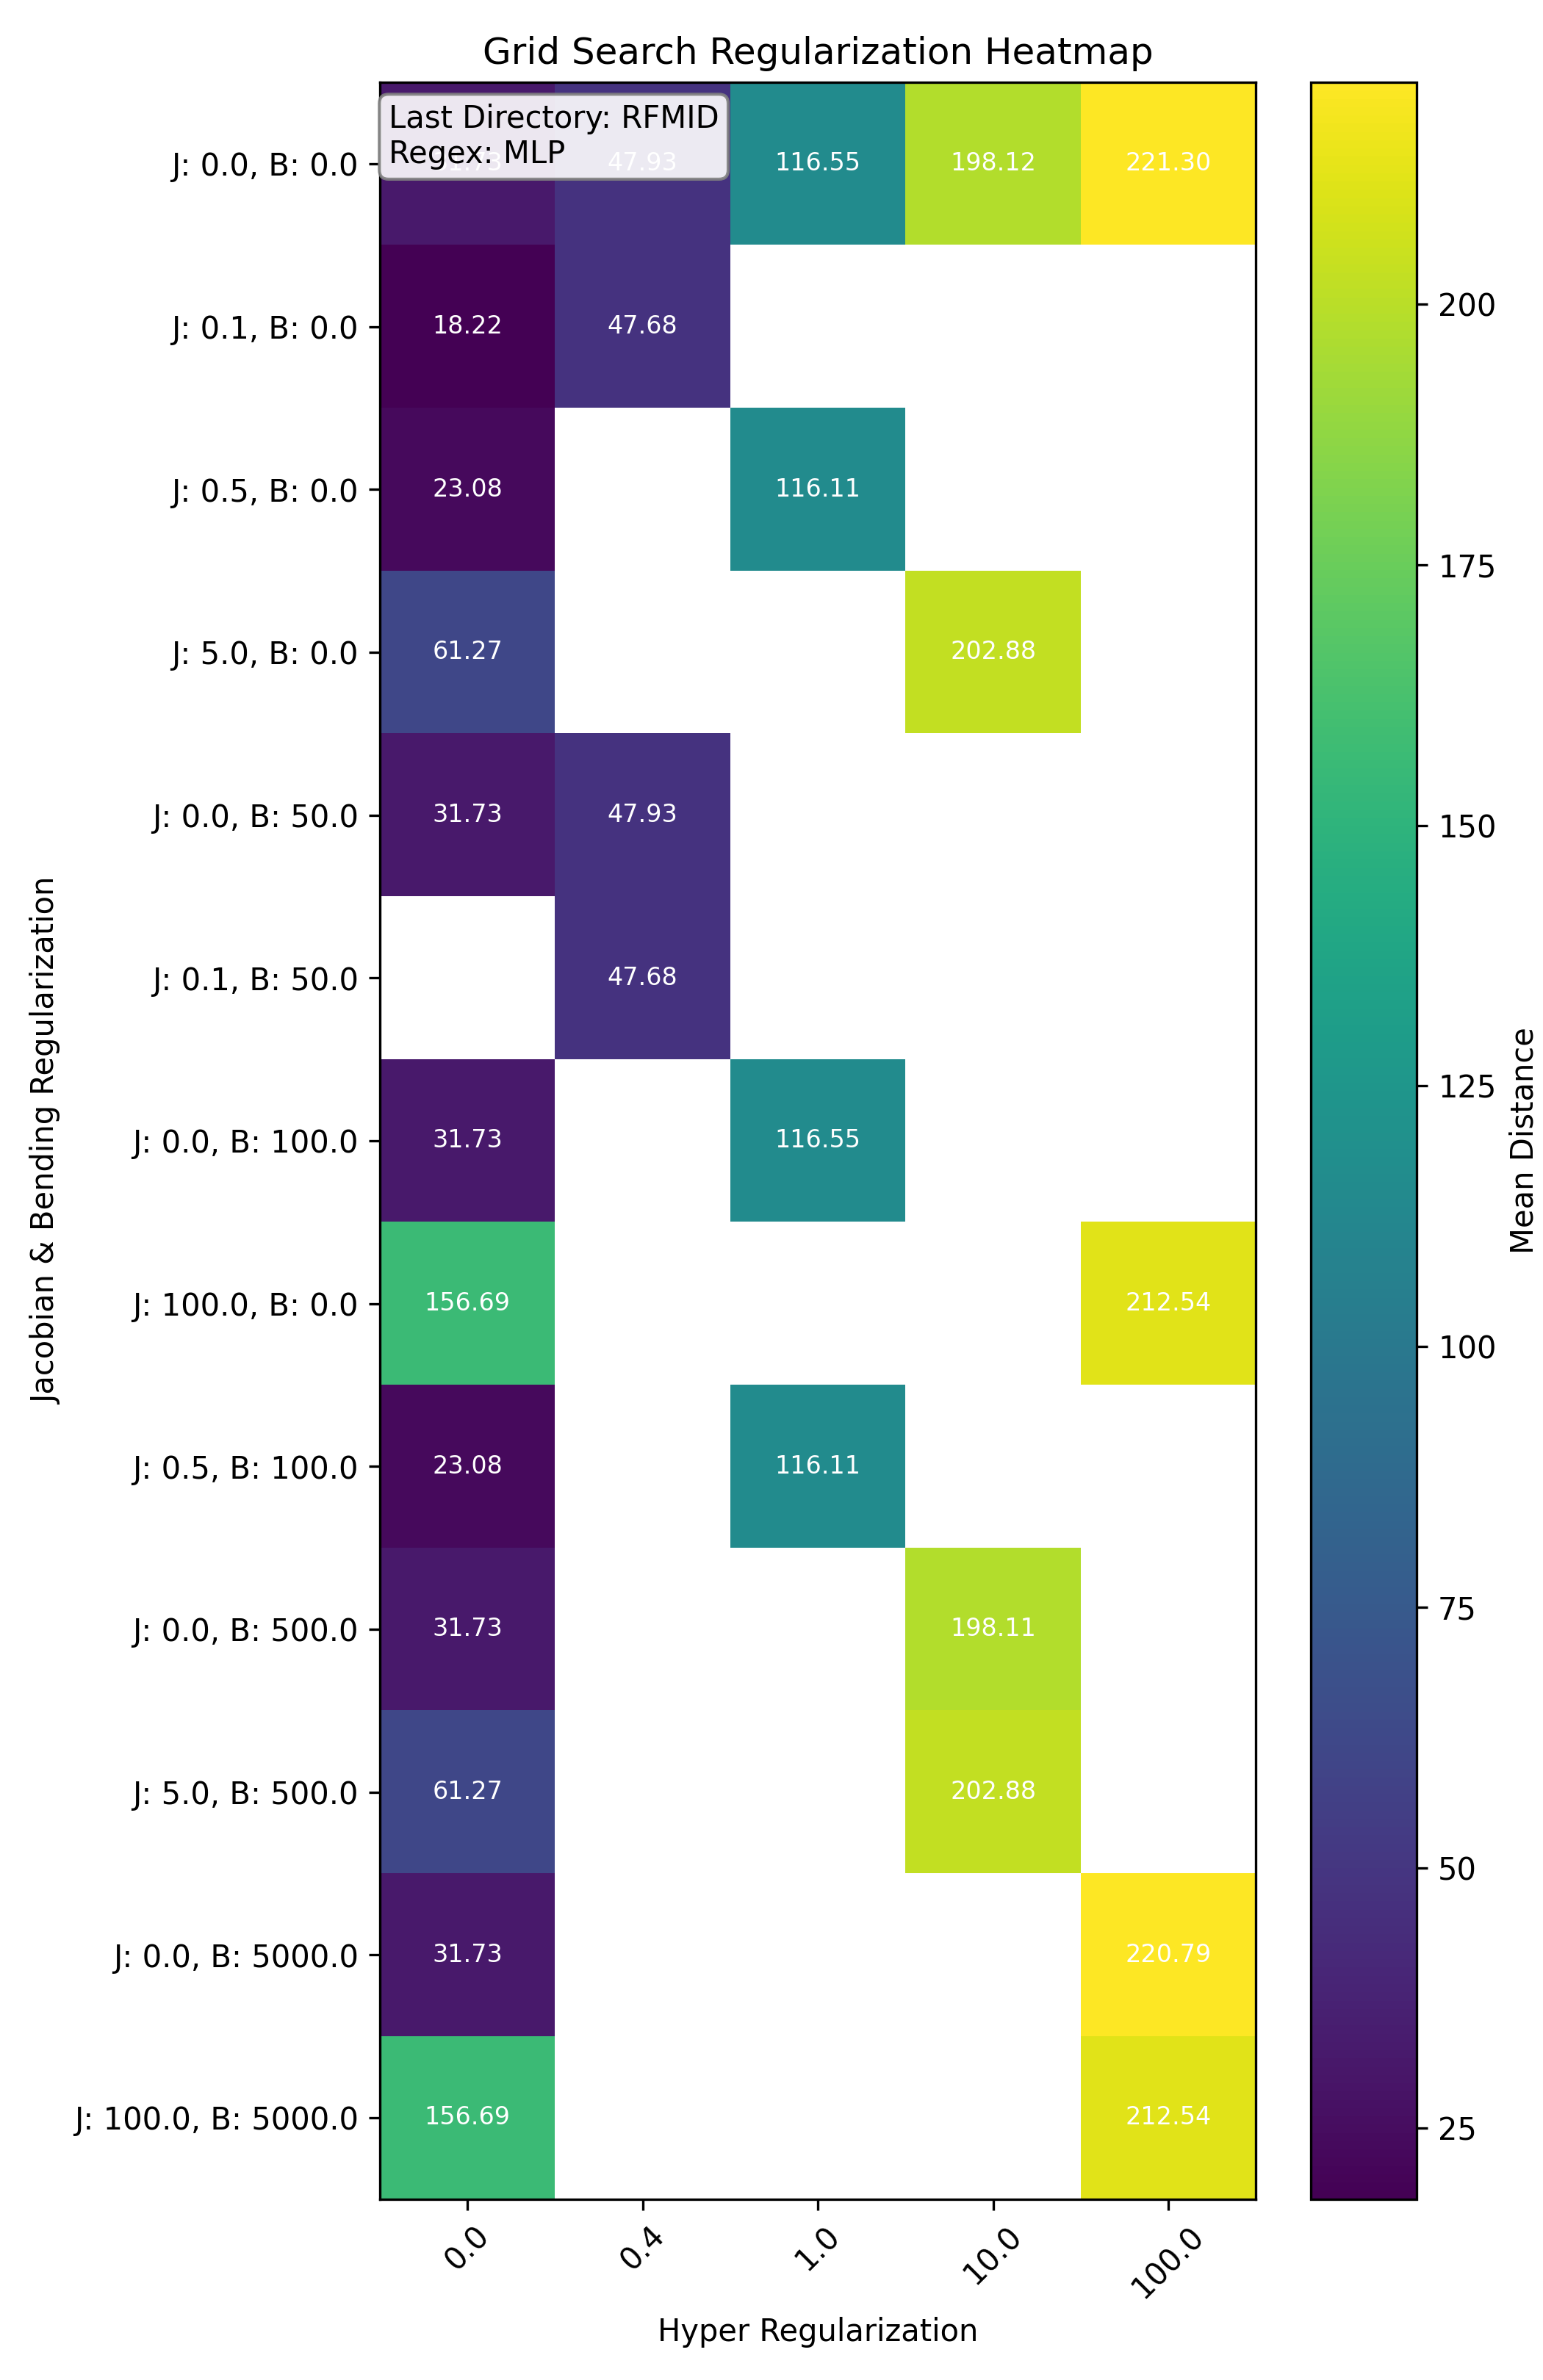
\includegraphics[width=\textwidth]{imaxes/grid_search_single_heatmap_RFMID_MLP.png}
        \caption{RFMID - Relu}
        \label{fig:gs_single_RFMID_MLP}
    \end{subfigure}\hfill
    \begin{subfigure}[b]{0.4\textwidth}
        \centering
        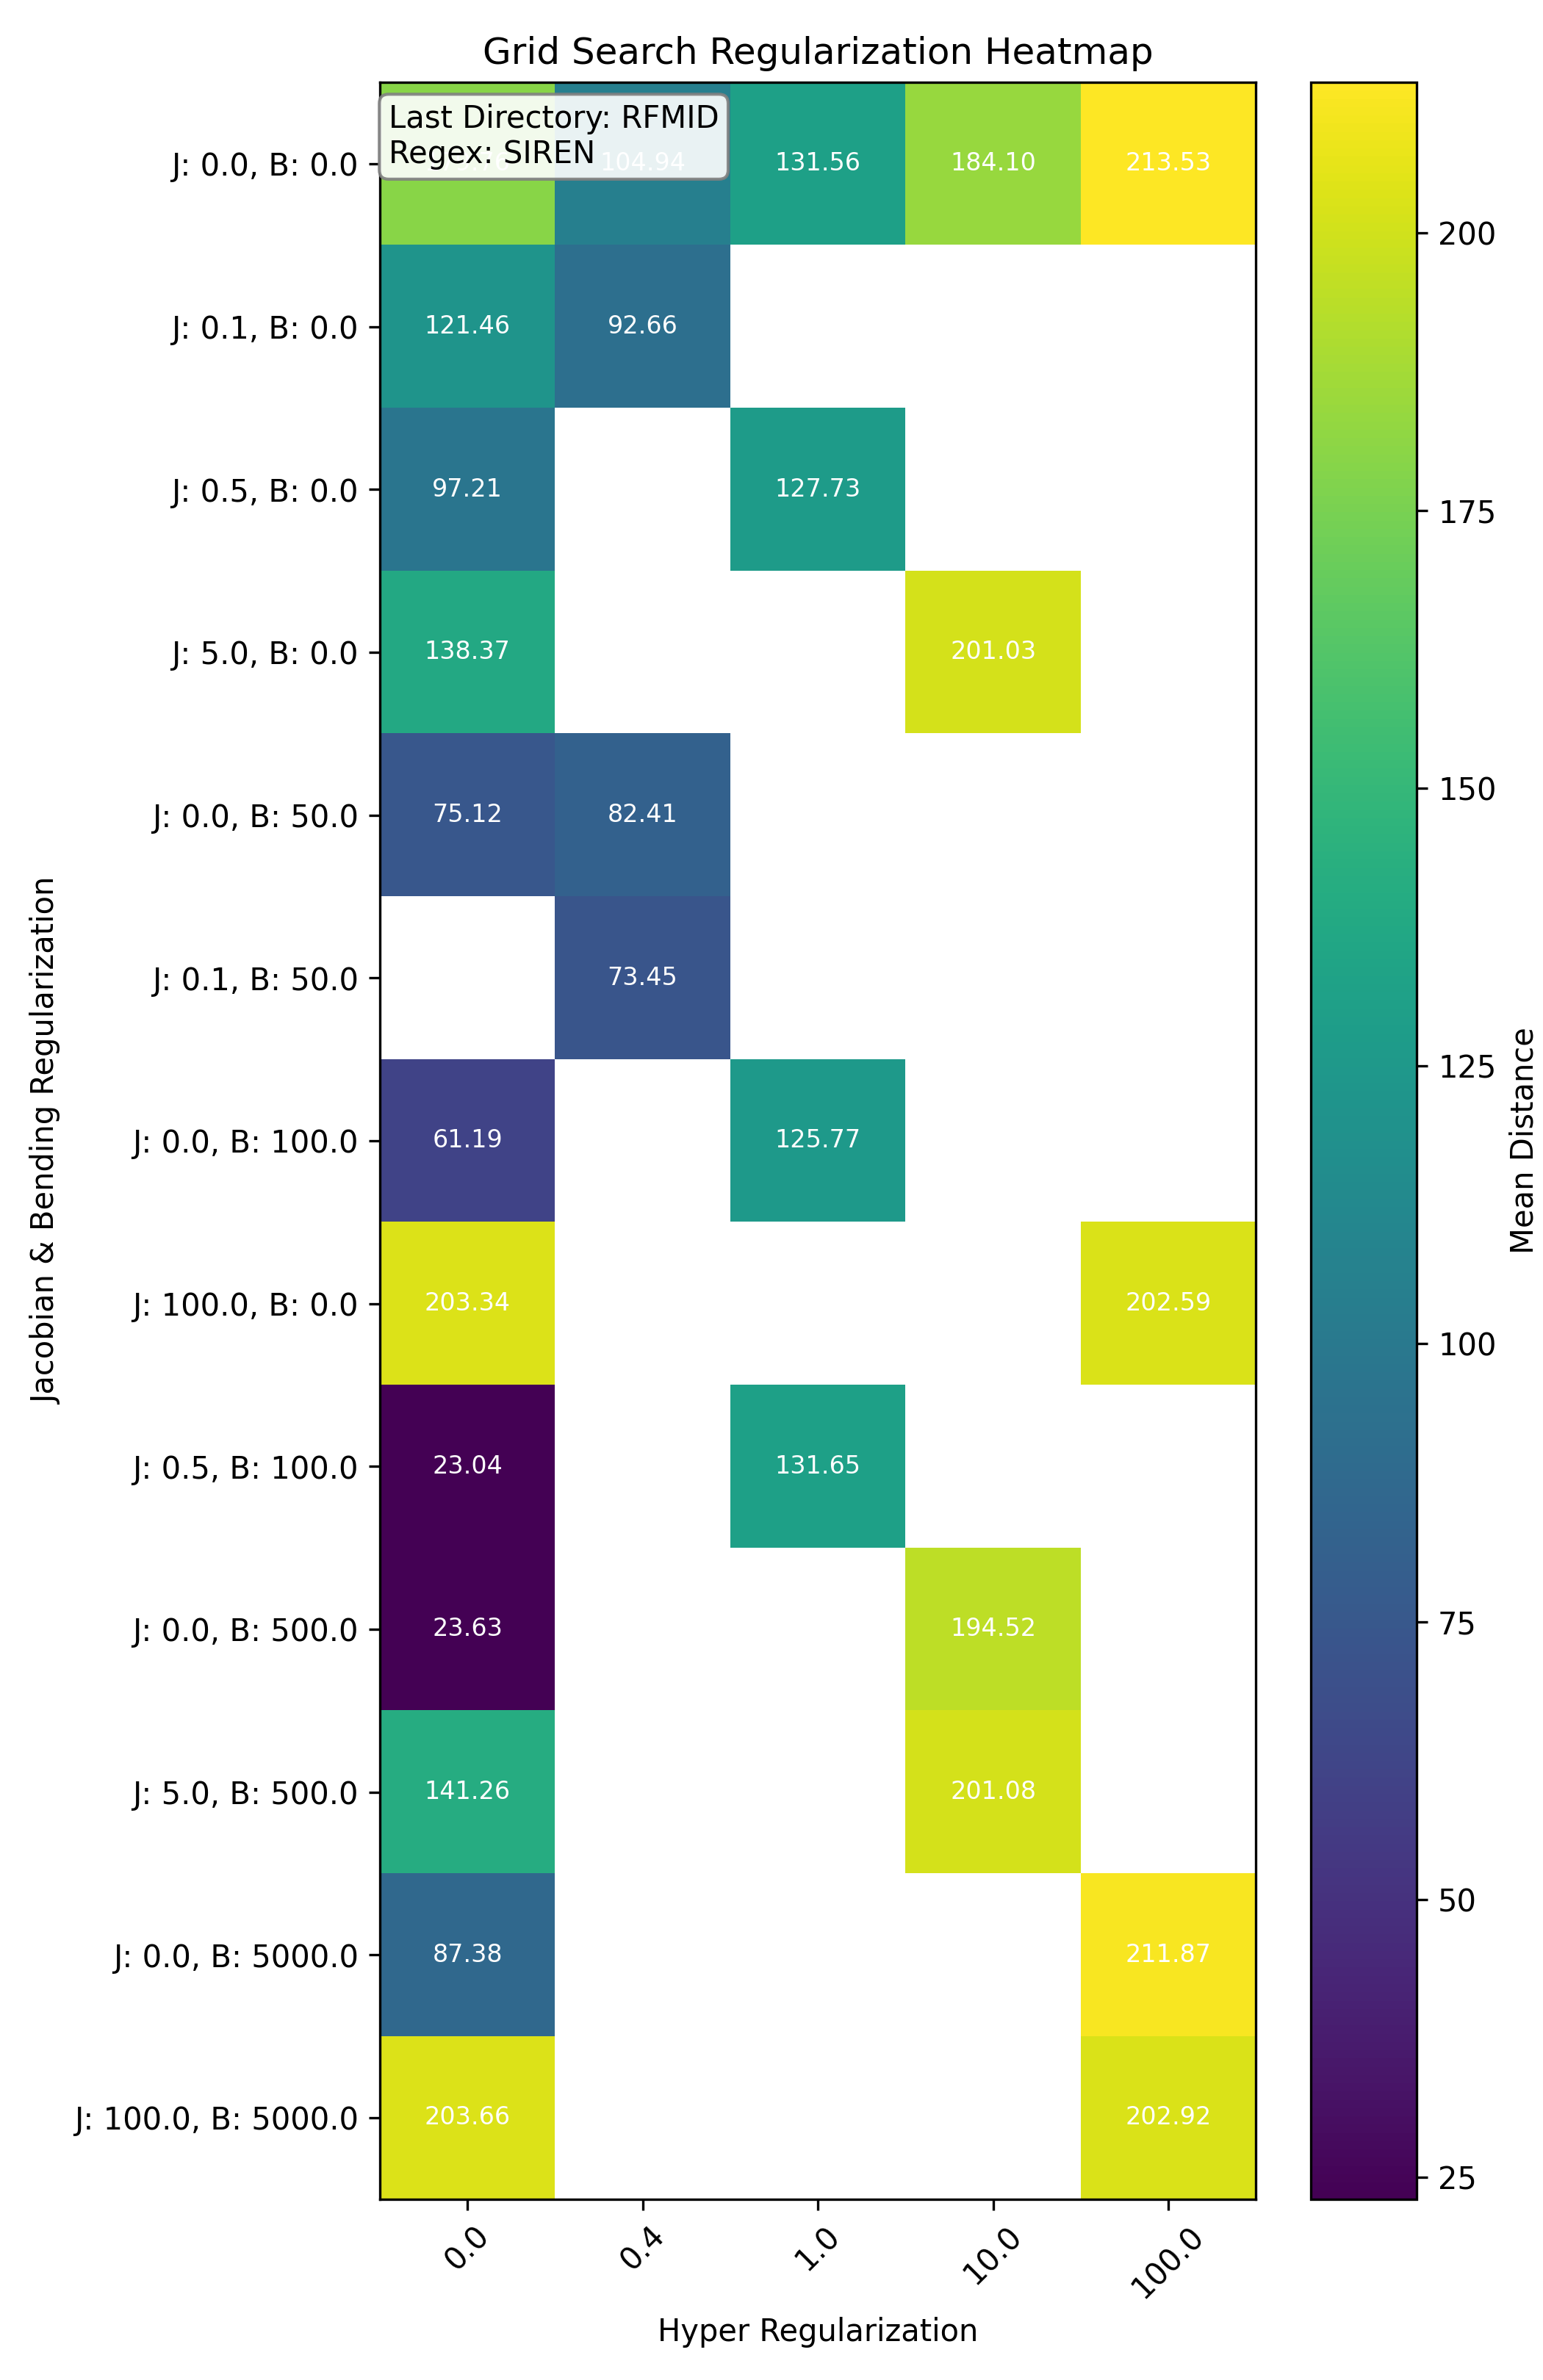
\includegraphics[width=\textwidth]{imaxes/grid_search_single_heatmap_RFMID_SIREN.png}
        \caption{RFMID - SIREN}
        \label{fig:gs_single_RFMID_SIREN}
    \end{subfigure}
    
    \caption{Mapa de calor cos resultados de diferentes combinacións de termos de regularización e funcións de activación sobre os datasets FIRE e RFMID}
    \label{fig:gs_single_heatmaps}
\end{figure}

\paragraph{Discusión}
\label{par:Discusion-reg2}

Os resultados amosan que as interaccións entre os diferentes termos de regularización e as funcións de activación son complexas e moi dependentes da parella de imaxes concreta a rexistrar.

\FloatBarrier

 \printglossary[type=\acronymtype,title=\nomeglosarioacronimos]
 \printglossary[title=\nomeglosariotermos]

 \bibliographystyle{IEEEtranN}
 \bibliography{\bibconfig,bibliografia/bibliografia}
 \clearpage
 
\end{document}

%%%%%%%%%%%%%%%%%%%%%%%%%%%%%%%%%%%%%%%%%%%%%%%%%%%%%%%%%%%%%%%%%%%%%%%%%%%%%%%%
